\documentclass[a4paper,13pt]{report}

%% Packages
\usepackage[a4paper,top=2cm,bottom=2cm,left=3cm,right=2cm]{geometry}
\usepackage{graphicx}
\usepackage{float}
\usepackage[utf8]{inputenc}
\usepackage{etoolbox}
\usepackage{tikz}
\usepackage{fancyhdr}
\usetikzlibrary{calc}
\usepackage{tocloft}
\usepackage[utf8]{vietnam}
\usepackage{titlesec}
\usepackage{everypage}
\usepackage{afterpage}
\usepackage[vietnamese]{babel} 
\usepackage{times} %Times Font
\usepackage{atbegshi}
\usepackage{titletoc}
\usepackage[nonumberlist, nopostdot, nogroupskip, acronym]{glossaries}
\usepackage{glossary-superragged}
\setglossarystyle{superraggedheaderborder}
\usepackage{setspace}
\usepackage{parskip}
\usepackage{glossaries}
\usepackage{longtable}
\usepackage{truncate} 
\usepackage{hyperref}
%\usepackage{hyperref}


\renewcommand{\bibname}{Danh_sach_tai_lieu_tham_khao} 
\usepackage[backend=bibtex,style=ieee]{biblatex}  %backend=biber is 'better'

\addbibresource{Danh_sach_tai_lieu_tham_khao.bib} % 



\renewcommand{\baselinestretch}{1.5}

\def\PageTopMargin{0in}
\def\PageLeftMargin{0in}
\newcommand\atxy[3]{
    \AddThispageHook{
        \smash{
            \hspace*{
                \dimexpr-\PageLeftMargin-\hoffset+#1\relax
            }
            \raisebox{
                \dimexpr\PageTopMargin+\voffset-#2\relax
            }{#3}
        }
    }
}

% package content table
\titleformat{\chapter}[hang]{\centering\bfseries}{CHƯƠNG \thechapter.\ }{0pt}{}[]
\titleformat 
    {\chapter} % command
    [hang] % shape
    {\centering\bfseries} % format
    {CHƯƠNG \thechapter.\ } % label
    {0pt} %sep
    {} % before
    [] % after
\titlespacing*{\chapter}{0pt}{-20pt}{20pt}

\titleformat
    {\section} % command
    [hang] % shape
    {\bfseries} % format
    {\thechapter.\arabic{section}\ \ \ \ } % label
    {0pt} %sep
    {} % before
    [] % after
\titlespacing{\section}{0pt}{\parskip}{0.5\parskip}

\titleformat
    {\subsection} % command
    [hang] % shape
    {\bfseries} % format
    {\thechapter.\arabic{section}.\arabic{subsection}\ \ \ \ } % label
    {0pt} %sep
    {} % before
    [] % after
\titlespacing{\subsection}{30pt}{\parskip}{0.5\parskip}

\renewcommand\thesubsubsection{\alph{subsubsection}}
\titleformat
    {\subsubsection} % command
    [hang] % shape
    {\bfseries} % format
    {\alph{subsubsection}, \ } % label
    {0pt} %sep
    {} % before
    [] % after
\titlespacing{\subsubsection}{50pt}{\parskip}{0.5\parskip}

\renewcommand{\contentsname}{\centering\Large\MakeUppercase{Mục lục} }
\renewcommand{\cfttoctitlefont}{\hfill\Large\bfseries\MakeUppercase} % Căn giữa và làm đậm tiêu đề mục lục
\renewcommand{\cftaftertoctitle}{\hfill} % Căn giữa tiêu đề mục lục
\renewcommand{\cftchapleader}{\cftdotfill{\cftdotsep}} % Chấm dẫn dưới mục chương
\titlecontents{chapter}
    [0.0cm]             % left margin
    {\bfseries\vspace{0.3cm}}                  % above code
    {{\bfseries{\scshape} CHƯƠNG \thecontentslabel.\ }} % numbered format
    {}         % unnumbered format
    {\titlerule*[0.3pc]{.}\contentspage}         % filler-page-format, e.g dots


\titlecontents{section}
    [0.0cm]             % left margin
    {\vspace{0.3cm}}                  % above code
    {\thecontentslabel \ } % numbered format
    {}         % unnumbered format
    {\titlerule*[0.3pc]{.}\contentspage}         % filler-page-format, e.g dots
\titlecontents{subsection}
    [1.0cm]             % left margin
    {\vspace{0.3cm}}                  % above code
    {\thecontentslabel \ } % numbered format
    {}         % unnumbered format
    {\titlerule*[0.3pc]{.}\contentspage}         % filler-page-format, e.g dots


\makeglossaries
%\makenoidxglossaries
\newlength{\glscolwidthA}
\newlength{\glscolwidthB}
\setlength{\glscolwidthA}{2cm} % Độ rộng cột name
\setlength{\glscolwidthB}{\dimexpr\linewidth-\glscolwidthA-4\tabcolsep} % Độ rộng cột description

\newglossarystyle{mylist}{%
    \setglossarystyle{long}% sử dụng longtable style
    \renewenvironment{theglossary}%
        {\begin{longtable}{p{\glscolwidthA}p{\glscolwidthB}}}%
        {\end{longtable}}%
    \renewcommand*{\glossaryheader}{}%
    \renewcommand*{\glsgroupheading}[1]{}%
    \renewcommand*{\glsgroupskip}{}%
    \renewcommand{\glossentry}[2]{%
        \glstarget{##1}{\glossentryname{##1}} & \glossentrydesc{##1}\tabularnewline
    }%
}


% Danh mục thuật ngữ và từ viết tắt
\newglossaryentry{iaas}{
    type=\acronymtype,
    name={IaaS: Infrastructure  as  a  Service},
    description={Dịch vụ hạ tầng},
    first={Dịch vụ hạ tầng}
}
\newglossaryentry{API}{
    type=\acronymtype,
    name={API: Application Programming Interface},
    description={Giao diện lập trình ứng dụng},
    first={API}
}
\newglossaryentry{EUD}{
    type=\acronymtype,
    name={EUD: End-User Development},
    description={Phát triển ứng dụng người dùng cuối},
    first={End-User Development}
}
\newglossaryentry{GWT}{
    type=\acronymtype,
    name={GWT: Google Web Toolkit},
    description={Công cụ lập trình Javascript bằng Java của Google},
    first={Công cụ lập trình Javascript bằng Java của Google (Google Web Toolkit}
}
\newglossaryentry{HTML}{
    type=\acronymtype,
    name={HTML: HyperText Markup Language},
    description={Ngôn ngữ đánh dấu siêu văn bản},
    first={Dịch vụ hạ tầng (Infrastructure  as  a  Service - IaaS)}
}

% =========================== BODY ===============
\begin{document}

%\sloppy
\pagestyle{fancy}
\fancyhf{}
\fancyhead[L]{NHÓM 12 - LỚP N04 } % Di chuyển header về bên trái
\renewcommand{\headrulewidth}{0.4pt} % Gạch dưới header

\fancyfoot[R]{\roman{page}} % Số trang theo chữ số La mã ở bên phải của footer


\pagenumbering{gobble}


\newgeometry{top=2cm,bottom=2cm,left=3cm,right=2cm} 
\thispagestyle{empty}
\atxy{0.55cm}{0.7cm}{
    \rotatebox[origin=l]{-90}{
        \makebox[9.75in]{
            \parbox{9.75in}{
               \large{ NHẬP MÔN KHOA HỌC DỮ LIỆU}
                \hspace*{3.25cm}
                \large{NHÓM 12 - LỚP N04}
                \rule[0pt]{0pt}{0pt}
            }
        }
    }
}
\begin{tikzpicture}[overlay,remember picture]
\draw[blue, line width=2.75pt]
    ($ (current page.north west) + (4.5cm,-1.5cm) $)
    rectangle
    ($ (current page.south east) + (-1cm,3cm) $);
    \draw[ line width=0.5pt]
    ($ (current page.north west) + (4.5cm,-1.5cm) $)
    rectangle
    ($ (current page.south east) + (-1cm,3cm) $);
    \draw[line width=1.25pt]
    ($ (current page.north west) + (4.55cm,-1.55cm) $)
    rectangle
    ($ (current page.south east) + (-1.05cm,3.05cm) $);
    \draw[line width=2pt]
    ($ (current page.north west) + (3cm,-1.5cm) $)
    rectangle
    ($ (current page.south east) + (-16.5cm,3cm) $);
%\draw[line width=2pt]
%    ($ (current page.north west) + (1.2cm,-1.2cm) $)
%    rectangle
%    ($ (current page.south east) + (-1.2cm,1.2cm) $);
\end{tikzpicture}
\begin{center}
\hspace*{3cm} {\textbf{\large{BỘ THÔNG TIN VÀ TRUYỀN THÔNG}}}\\
\vspace{0.3cm}
\hspace*{3cm}  {\textbf{\large{HỌC VIỆN CÔNG NGHỆ BƯU CHÍNH VIỄN THÔNG}}}\\
\hspace*{3cm} {\textbf{\large{\underline{\hspace{6cm}}}}}\\
\vspace{0.7cm}
\hspace*{3cm} 
\includegraphics[width=0.3\linewidth]{ptit_logo_1.png}
\\
\vspace{0.7cm}
\hspace*{3cm}\linespread{1}\large\textbf{BÁO CÁO DỰ ÁN}\\
\hspace*{3cm}\linespread{1}\large\textbf {NHẬP MÔN KHOA HỌC DỮ LIỆU}
\vspace{1cm}
\\
\hspace*{2cm} \textbf{\textit{Đề tài:}  “HỆ THỐNG ĐỀ XUẤT KHÁCH SẠN HÀ NỘI DỰA TRÊN}
\\ \hspace*{2cm} \textbf{\hspace*{2cm} ĐÁNH GIÁ KHÁCH HÀNG TRƯỚC ĐÓ ” }

\vspace{1in}

\begin{tabular}{ll}
{\textbf{\large{Nhóm 12 :}}}  & {\textbf{\large{NO4}}} \\
{\textbf{\large{Người hướng dẫn : }}} & {\textbf{\large{TS. Đinh Xuân Trường}}} \\
{\textbf{\large{Trần Đức Thịnh}}} & {\textbf{\large{: B21DCCN693}}}  \\
{\textbf{\large{Vũ Danh Phong}}} & {\textbf{\large{: B21DCCN590}}}  \\
{\textbf{\large{Trần Đức Huy}}} & {\textbf{\large{: B21DCCN440}}}  \\
{\textbf{\large{Trần Quang Huy}}} & {\textbf{\large{: B21DCCN441}}}  \\


\end{tabular}


\vspace{1in}

\hspace*{3cm} \textbf{HÀ NỘI - 2024}
\end{center}
\newgeometry{top=1.5cm,bottom=2cm,left=3cm,right=2cm} 
\thispagestyle{empty}
\begin{tikzpicture}[overlay,remember picture]
    \draw[line width=2pt]
    ($ (current page.north west) + (3cm,-1.5cm) $)
    rectangle
    ($ (current page.south east) + (-1cm,3cm) $);
%\draw[line width=2pt]
%    ($ (current page.north west) + (1.2cm,-1.2cm) $)
%    rectangle
%    ($ (current page.south east) + (-1.2cm,1.2cm) $);
\end{tikzpicture}
\begin{center}
\hspace*{1cm} {\textbf{\large{BỘ THÔNG TIN VÀ TRUYỀN THÔNG}}}\\
\vspace{0.3cm}
\hspace*{1cm}  {\textbf{\large{HỌC VIỆN CÔNG NGHỆ BƯU CHÍNH VIỄN THÔNG}}}\\
\hspace*{1cm} {\textbf{\large{\underline{\hspace{6cm}}}}}\\
\vspace{0.7cm}
\hspace*{1cm} 
\includegraphics[width=0.3\linewidth]{ptit_logo_1.png}
\\
\vspace{0.7cm}
\hspace*{1cm}\linespread{1}\large\textbf {BÁO CÁO DỰ ÁN}\\
\hspace*{1cm}\linespread{1}\large\textbf{NHẬP MÔN KHOA HỌC DỮ LIỆU}
\vspace{1cm}
\\
\hspace*{1cm} \textbf{\textit{Đề tài:}  “ HỆ THỐNG ĐỀ XUẤT KHÁCH SẠN HÀ NỘI DỰA TRÊN}
\\ \hspace*{1cm} \textbf{\hspace*{2cm} ĐÁNH GIÁ KHÁCH HÀNG TRƯỚC ĐÓ ” }

\vspace{1in}

\begin{tabular}{ll}
{\textbf{\large{Nhóm 12 :}}}  & {\textbf{\large{NO4}}} \\
{\textbf{\large{Trần Đức Thịnh}}} & {\textbf{\large{: B21DCCN693}}}  \\
{\textbf{\large{Vũ Danh Phong}}} & {\textbf{\large{: B21DCCN590}}}  \\
{\textbf{\large{Trần Đức Huy}}} & {\textbf{\large{: B21DCCN440}}}  \\
{\textbf{\large{Trần Quang Huy}}} & {\textbf{\large{: B21DCCN441}}}  \\


\end{tabular}


\end{center}
%\newgeometry{top=2.5cm,bottom=2cm,left=3cm,right=2cm} 
\thispagestyle{empty}
\begin{center}
    {\textbf{\Large{NHẬN XÉT CỦA GIẢNG VIÊN HƯỚNG DẪN}}}
\end{center}

\dotfill \vspace{0.25cm} \par
\dotfill \vspace{0.25cm} \par
\dotfill \vspace{0.25cm} \par
\dotfill \vspace{0.25cm} \par
\dotfill \vspace{0.25cm} \par
\dotfill \vspace{0.25cm} \par
\dotfill \vspace{0.25cm} \par
\dotfill \vspace{0.25cm} \par
\dotfill \vspace{0.25cm} \par
\dotfill \vspace{0.25cm} \par
\dotfill \vspace{0.25cm} \par
\dotfill \vspace{0.25cm} \par
\dotfill \vspace{0.25cm} \par
\dotfill \vspace{0.25cm} \par
\dotfill \vspace{0.25cm} \par
\dotfill \vspace{0.25cm} \par
\dotfill \vspace{0.25cm} \par
\dotfill \vspace{0.25cm} \par
\dotfill

\vspace{1cm}

{\textbf{\large{Điểm: }}} \hspace{1.0cm}\textbf{( Bằng chữ:}  \hspace{2.5cm}\textbf{)}  

\begin{flushright}
Hà Nội, ngày \hspace{0.75cm} tháng \hspace{0.75cm} năm 20...\hspace{0.75cm}

{\textbf{\large{Giảng viên hướng dẫn }}} \hspace{1cm} \textcolor{white}{.}
\end{flushright}
%\newgeometry{top=2.5cm,bottom=2cm,left=3cm,right=2cm} 
\thispagestyle{empty}
\begin{center}
    {\textbf{\Large{NHẬN XÉT CỦA GIẢNG VIÊN PHẢN BIỆN: }}}
\end{center}

\dotfill \vspace{0.25cm} \par
\dotfill \vspace{0.25cm} \par
\dotfill \vspace{0.25cm} \par
\dotfill \vspace{0.25cm} \par
\dotfill \vspace{0.25cm} \par
\dotfill \vspace{0.25cm} \par
\dotfill \vspace{0.25cm} \par
\dotfill \vspace{0.25cm} \par
\dotfill \vspace{0.25cm} \par
\dotfill \vspace{0.25cm} \par
\dotfill \vspace{0.25cm} \par
\dotfill \vspace{0.25cm} \par
\dotfill \vspace{0.25cm} \par
\dotfill \vspace{0.25cm} \par
\dotfill \vspace{0.25cm} \par
\dotfill \vspace{0.25cm} \par
\dotfill \vspace{0.25cm} \par
\dotfill \vspace{0.25cm} \par
\dotfill

\vspace{1cm}

{\textbf{\large{Điểm: }}} \hspace{1.0cm}\textbf{( Bằng chữ:}  \hspace{2.5cm}\textbf{)}  

\begin{flushright}
Hà Nội, ngày \hspace{0.75cm} tháng \hspace{0.75cm} năm 20...\hspace{0.75cm}

{\textbf{\large{Giảng viên phản biện }}} \hspace{1cm} \textcolor{white}{.}
\end{flushright}

%\clearpage % Tạo trang mới
% Thêm trang Lời cảm ơn vào Mục lục

\pagenumbering{roman}
\addcontentsline{toc}{chapter}{LỜI CẢM ƠN}
\newgeometry{top=2cm,bottom=2cm,left=3cm,right=2cm} 

\thispagestyle{fancy}

\begin{center}
    \Large{\textbf{LỜI CẢM ƠN}}\\
\end{center}
\vspace{0.5cm}
\hspace{0.7cm} Lời đầu tiên, nhóm em xin được gửi lời cảm ơn sâu sắc nhất tới thầy vì sự tận tâm và nhiệt huyết trong việc giảng dạy và hướng dẫn nhóm em suốt quá trình thực hiện bài tập lớn môn nhập môn khoa học dữ liệu. Nhờ có sự chỉ bảo chi tiết, sự kiên nhẫn và sự hỗ trợ vô giá của thầy, chúng em không chỉ có cơ hội tiếp cận và áp dụng các kiến thức mới mà còn hiểu rõ hơn về tầm quan trọng và ứng dụng thực tế của khoa học dữ liệu.

\hspace{0.7cm} Thầy đã luôn là nguồn động lực để chúng em vượt qua khó khăn, khơi dậy niềm đam mê và định hướng con đường học tập, phát triển tư duy khoa học. Những kiến thức và bài học mà thầy truyền đạt không chỉ giúp chúng em hoàn thành môn học mà còn tạo nền tảng vững chắc cho những bước tiến trong sự nghiệp tương lai của.

\hspace{0.7cm} Chúng em hiểu rằng mỗi thành công trong quá trình học tập đều có phần đóng góp lớn từ thầy, từ những lời khuyên bổ ích, sự chỉ dẫn tỉ mỉ cho đến tình cảm và lòng nhiệt huyết trong từng buổi học. Một lần nữa, chúng em xin gửi lời tri ân chân thành nhất đến thầy và hy vọng rằng thầy sẽ tiếp tục là nguồn cảm hứng lớn lao cho nhiều thế hệ sinh viên sau này.

\hspace{0.7cm} Kính chúc thầy sức khỏe và thành công trên con đường sự nghiệp giáo dục, để tiếp tục lan tỏa kiến thức và đam mê đến những sinh viên tiếp theo.

\vspace{4cm}
\begin{flushright}
Hà Nội, ngày 14\hspace{0.05cm} tháng 11\hspace{0.05cm} năm 2024\hspace{0.05cm}

{\textbf{\large{Đại diện nhóm }}} \hspace{1.2cm} \textcolor{white}{.}

\vspace{1.5cm}

{\textbf{\large{Trần Đức Thịnh}}} \hspace{1.2cm} \textcolor{white}{.}
\end{flushright}




% Thêm không gian trước mục lục
\thispagestyle{fancy}
% Tạo mục lục tự động
\addcontentsline{toc}{chapter}{MỤC LỤC}
\tableofcontents


% Tạo khối văn bản dưới tiêu đề mục lục

%DANH MỤC CÁC KÝ HIỆU VÀ CHỮ VIẾT TẮT
\glsaddall 
% \renewcommand*{\glossaryname}{Danh sách thuật ngữ}
\renewcommand*{\acronymname}{\Large DANH MỤC THUẬT NGỮ VÀ TỪ VIẾT TẮT}
\renewcommand*{\entryname}{\centering \hspace{1.75cm} Thuật ngữ}
\renewcommand*{\descriptionname}{\centering Ý nghĩa}
\addcontentsline{toc}{chapter}{DANH MỤC CÁC KÝ HIỆU VÀ CHỮ VIẾT TẮT}
\printglossaries

% \phantomsection\addcontentsline{toc}{section}{\numberline {} DANH MỤC THUẬT NGỮ VÀ TỪ VIẾT TẮT}


% Tạo danh mục các hình vẽ
\newpage
\thispagestyle{fancy}
\vspace*{-2.5cm} % Thay đổi giá trị để điều chỉnh khoảng cách
\addcontentsline{toc}{chapter}{ DANH MỤC CÁC HÌNH VẼ}
% Đổi tên danh mục hình vẽ thành "DANH MỤC HÌNH VẼ" và căn giữa tiêu đề
\renewcommand{\listfigurename}{\centering\Large\MakeUppercase{\hspace{5.5cm} DANH MỤC HÌNH VẼ}}
\listoffigures

%DANH MỤC CÁC BẢNG
\newpage
\thispagestyle{fancy}
\vspace*{-2.5cm} % Thay đổi giá trị để điều chỉnh khoảng cách
\addcontentsline{toc}{chapter}{DANH MỤC CÁC BẢNG}
\renewcommand{\listtablename}{\centering\Large\MakeUppercase{\hspace{5cm} DANH MỤC BẢNG BIỂU}}
\listoftables
% \phantomsection\addcontentsline{toc}{section}{\numberline {} DANH MỤC BẢNG BIỂU}
\newpage
\addcontentsline{toc}{chapter}{PHẦN MỞ ĐẦU}
\begin{center}
    \textbf{\Large PHẦN MỞ ĐẦU}
\end{center}
\textbf{Mục tiêu và định hướng cá nhân về quá trình thực tập cơ sở}: Trong quá trình thực tập cơ sở, mục tiêu của tôi là củng cố những kiến thức đã học và phát triển khả năng ứng dụng công nghệ vào các bài toán thực tế. Một trong những định hướng của tôi là phát triển các hệ thống thông minh, hỗ trợ người dùng tìm kiếm thông tin nhanh chóng và chính xác. Dự án này đóng vai trò quan trọng trong việc cung cấp giải pháp cho ngành du lịch, cụ thể là đề xuất khách sạn tại Hà Nội dựa trên nhu cầu của người dùng. Lý do tôi chọn đề tài này là vì du lịch đang trở thành ngành phát triển mạnh tại Việt Nam, và công nghệ thông tin có thể giúp tối ưu hóa trải nghiệm của du khách.

\textbf{\textit{Trình bày phần đặt vấn đề liên quan đến đề tài của TTCS: }} Công nghiệp 4.0 đang thúc đẩy sự phát triển mạnh mẽ của các ứng dụng công nghệ trong mọi lĩnh vực của cuộc sống. Ngành du lịch và dịch vụ cũng không nằm ngoài xu hướng này, đặc biệt trong việc tối ưu hóa trải nghiệm khách hàng. Trong bối cảnh đó, hệ thống gợi ý khách sạn thông minh dựa trên nhu cầu của người dùng có thể giúp du khách dễ dàng tìm kiếm và lựa chọn nơi lưu trú phù hợp.

\textbf{\textit{Trình bày phần các giải pháp hiện tại và hạn chế: }}  Hiện tại, các hệ thống gợi ý khách sạn phổ biến như Booking.com hay Agoda đã cung cấp nhiều lựa chọn phong phú, nhưng phần lớn dựa trên đánh giá người dùng hoặc xếp hạng sao. Những phương pháp này có thể không hoàn toàn phản ánh được nhu cầu thực sự của từng cá nhân trong từng thời điểm. Một số du khách vẫn phải tìm kiếm thủ công, gây mất thời gian.

\textbf{\textit{Trình bày phần mục tiêu và hướng giải pháp:}}  Để giải quyết vấn đề này, hệ thống đề xuất khách sạn thông minh dựa trên input từ người dùng sẽ giúp tự động gợi ý các khách sạn phù hợp nhất. Hệ thống này không chỉ giúp du khách tiết kiệm thời gian tìm kiếm mà còn mang lại trải nghiệm tốt hơn, cá nhân hóa hơn.

\textbf{\textit{Trình bày phần đóng góp của Đồ án và bố cục của Đồ án:}}  Hướng tới nhu cầu đó, đề tài đồ án tốt nghiệp có tên “\textbf{\textit{Ứng dụng nhận dạng ký tự quang cho bài toán nhận diện biển số xe}}”.

Nội dung trình bày trong báo cáo gồm 3 chương chính: 
\begin{itemize}
    \item Chương 1: Báo cáo tiến độ từng tuần trong quá trình training 
    \item Chương 2: Đề xuất và báo cáo đề tài Thực tập cơ sở bao gồm 3 nội dung:
    \begin{itemize}
        \item Giới thiệu chung: Trình bày tổng quan về đề tài, xác định mục tiêu xây dựng hệ thống đề xuất khách sạn tại Hà Nội dựa trên thông tin người dùng nhập vào. Đối tượng của hệ thống là du khách cần tìm kiếm nơi lưu trú tại Hà Nội. Phương hướng giải quyết là xây dựng một hệ thống gợi ý khách sạn thông minh, cá nhân hóa dựa trên thông tin như vị trí, ngân sách, loại hình khách sạn mong muốn. Hệ thống sẽ sử dụng các thuật toán gợi ý và phân tích dữ liệu để đưa ra kết quả tối ưu nhất. Giới thiệu các kiến thức liên quan về hệ thống gợi ý, xử lý dữ liệu và giao diện người dùng.
        \item Cơ sở lý thuyết: Tìm hiểu cơ sở lý thuyết về hệ thống gợi ý, bao gồm các thuật toán như collaborative filtering, content-based filtering, và hybrid recommendation systems. Phân tích các đặc điểm của ngành khách sạn tại Hà Nội như phân khúc giá, địa điểm, dịch vụ. Lựa chọn các thư viện và công cụ như Python, Pandas, Scikit-learn để tiến hành xây dựng mô hình gợi ý và ReactJS cho giao diện người dùng. 
    \item Xây dựng chương trình: Trình bày sơ đồ hệ thống, bao gồm các bước từ thu thập dữ liệu, tiền xử lý dữ liệu, xây dựng mô hình gợi ý, và phát triển giao diện người dùng. Sau đó, tiến hành đóng gói hệ thống và tích hợp vào website demo. Triển khai thực nghiệm, kiểm tra tính hiệu quả của hệ thống và đánh giá kết quả so với các phương pháp gợi ý truyền thống.
    \end{itemize}
    \item Chương 3: Kết luận quá trình Thực tập bao gồm Bài học và kết quả đạt được từ đó rút ra những điều cần cải thiện trong tương lai.
\end{itemize}





% ===================================================

\newpage
\pagenumbering{arabic}
\fancypagestyle{mainstyle}{
  \fancyhf{} % Xóa tất cả các header và footer hiện tại
  \fancyhead[L] {Nhập môn Khoa học dữ liệu} % Di chuyển header về bên trái
  \fancyhead[R]{\nouppercase{\truncate{0.5\headwidth}{\leftmark}}}
  \renewcommand{\headrulewidth}{0.4pt} % Độ dày của đường line phía trên header
  \renewcommand{\footrulewidth}{0.4pt} % Độ dày của đường line phía dưới footer
 \fancyfoot[L]{NHÓM 12 - LỚP N04 }
  \fancyfoot[R]{\thepage} % Hiển thị số trang ở bên phải
}
% Định nghĩa lệnh \shorttitle để cắt ngắn tiêu đề


\pagestyle{mainstyle}
\chapter {GIỚI THIỆU ĐỀ TÀI} 

\section{Tổng quan đề tài}
\subsection* {Khảo sát hiện trạng}
\label{sec:dvd}

Đề tài "Hệ thống gợi ý khách sạn tại Hà Nội" tập trung vào việc xây dựng một hệ thống cung cấp tên khách sạn dựa trên yêu cầu của người dùng. Nguồn dữ liệu được thu thập từ Tripadvisor.com, một nền tảng đánh giá khách sạn và dịch vụ du lịch uy tín. Lý do chọn đề tài này là nhằm giúp người dùng dễ dàng tìm kiếm các khách sạn phù hợp với nhu cầu cá nhân, từ đó tối ưu hóa trải nghiệm du lịch của họ. Việc nghiên cứu và xây dựng hệ thống này không chỉ có ý nghĩa thực tiễn trong việc hỗ trợ người dùng mà còn đóng góp vào phát triển các ứng dụng trí tuệ nhân tạo trong lĩnh vực du lịch.


\subsection*{Các giải pháp hiện tại và hạn chế}
\label{sec:giaiphap}
Hiện tại, các hệ thống gợi ý khách sạn phổ biến đều sử dụng các thuật toán máy học và trí tuệ nhân tạo để phân tích dữ liệu. Tuy nhiên, các hệ thống này vẫn gặp nhiều thách thức trong việc cá nhân hóa đề xuất cho từng người dùng do dữ liệu đầu vào đa dạng và phức tạp. Hệ thống của chúng tôi sẽ kế thừa và phát triển các phương pháp hiện có, đồng thời giải quyết những hạn chế như: độ chính xác của gợi ý, thời gian phản hồi, và tính đa dạng của dữ liệu.
\section{Mục tiêu và định hướng giải pháp}
Mục tiêu của đề tài là xây dựng một hệ thống gợi ý khách sạn tại Hà Nội dựa trên thông tin người dùng nhập vào, như vị trí, giá cả, loại hình khách sạn, và đánh giá từ các nguồn dữ liệu trên Tripadvisor.com. Hướng tiếp cận chính là sử dụng các thuật toán phân tích dữ liệu và học máy, kết hợp với kỹ thuật xử lý ngôn ngữ tự nhiên để tối ưu hóa độ chính xác của các gợi ý. 

\section{Đóng góp của tài}

Bài tập lớn này có 3 đóng góp chính như sau:

\begin{enumerate}
\item Khảo sát và phân tích các hệ thống gợi ý khách sạn hiện có, đồng thời chỉ ra các điểm mạnh và hạn chế.
\item Đề xuất phương pháp và quy trình xây dựng hệ thống gợi ý dựa trên dữ liệu từ Tripadvisor.com.
\item Phát triển một hệ thống gợi ý khách sạn có khả năng cá nhân hóa dựa trên đầu vào của người dùng.
\end{enumerate}

\section{Giới thiệu về bài toán xử lý ảnh}


\section{Giới thiệu về Deep learning}

\section{Đánh giá mô hình Deep learning}
\section*{Kết luận chương}
Chương này đã giới thiệu tổng quan về hệ thống gợi ý khách sạn tại Hà Nội, lý do chọn đề tài và mục tiêu nghiên cứu. Các thách thức trong việc triển khai hệ thống này cũng được thảo luận, cùng với các đóng góp quan trọng của đề tài. Ở chương tiếp theo, chúng tôi sẽ trình bày các kiến thức lý thuyết cơ bản liên quan đến hệ thống gợi ý và các phương pháp kỹ thuật sẽ được áp dụng.

% Khôi phục lại margin



% Phần mở đầu

\pagestyle{mainstyle}
\chapter{BÁO CÁO TIẾN ĐỘ TỪNG TUẦN Topic 1-12}
\textbf{\textit{Cần có phần tóm tắt mỗi khi bắt đầu chương}}\textit{Chương 2 giới thiệu bài toán nhận dạng ký tự quang và khảo sát các vấn đề nhận dạng biển số trong nhiều hệ thống khác nhau về các đặc điểm các dữ liệu ký tự quang. Trong đó, trình bày một số các nghiên cứu liên quan dến bài toán trên thế giới và trong nước, các khó khăn trong nghiên cứu bài toán để từ đó đặt ra mục tiêu và xác định nội dung nghiên cứu cho đồ án}.

\hspace{0.7cm}SV cần đặc biệt lưu ý cách hành văn. Mỗi đoạn văn không được quá dài và cần có ý tứ rõ ràng, bao gồm duy nhất một ý chính và các ý phân tích bổ trợ để làm rõ hơn ý chính. Các câu văn trong đoạn phải đầy đủ chủ ngữ vị ngữ, cùng hướng đến chủ đề chung. Câu sau phải liên kết với câu trước, đoạn sau liên kết với đoạn trước. Trong văn phong khoa học, sinh viên không được dùng từ trong văn nói, không dùng các từ phóng đại, thái quá, các từ thiếu khách quan, thiên về cảm xúc, về quan điểm cá nhân như “tuyệt vời”, “cực hay”, “cực kỳ hữu ích”, v.v. Các câu văn cần được tối ưu hóa, đảm bảo rất khó để thể thêm hoặc bớt đi được dù chỉ một từ. Cách diễn đạt cần ngắn gọn, súc tích, không dài dòng.

\section{Tổng quan quá trình làm dự án trong 12 tuần}
\subsection* {Nội dung thực tập trong 3 tháng }
Tiến độ thực hiện thực tập thể hiện trong bảng dưới đây:
\begin{figure}[h]
\centering
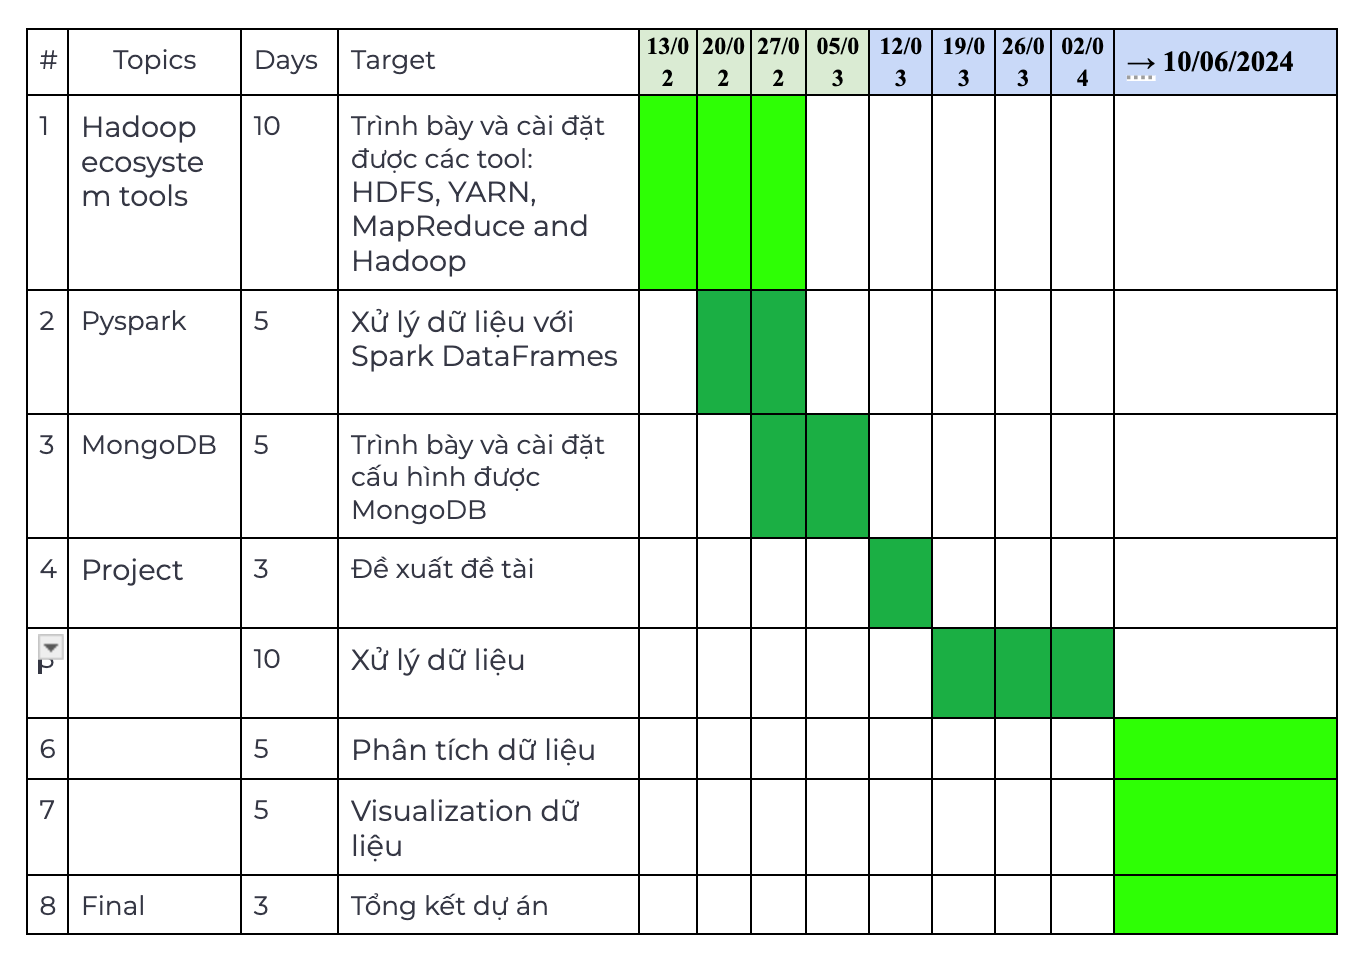
\includegraphics[width=1.0\linewidth]{Figures/Tiendo.png}
\caption {Tiến độ thực hiện thực tập}
\label{fig:iot}
\end{figure}

\section*{Tuần 4 (06/09 - 12/09)}
\subsection{Chủ đề tìm hiểu tuần 4:} Thu thập và tìm hiểu dữ liệu

\textbf{Mục tiêu tuần 4:} Thu thập được dữ liệu từ Tripadvisor.com

\textbf{Kết quả của tuần Topic:}
\begin{enumerate}
    \item Xác định đặc điểm kỹ thuật của trang web cần thu thập.
    \begin{enumerate}
        \item \textbf{Trang web cần thu thập là Booking.com}, chuyên cung cấp danh sách khách sạn tại Hà Nội, với các thông tin chi tiết về địa chỉ, giá phòng và đánh giá từ khách hàng. Hệ thống sẽ dựa trên những thông tin này để đề xuất khách sạn phù hợp cho khách hàng. Chi tiết hơn xem tại ảnh \hyperref[fig:image]{Hình 2.2}
        
        \begin{figure} % Sử dụng [H] để giữ hình ảnh ngay tại vị trí này
        \centering
        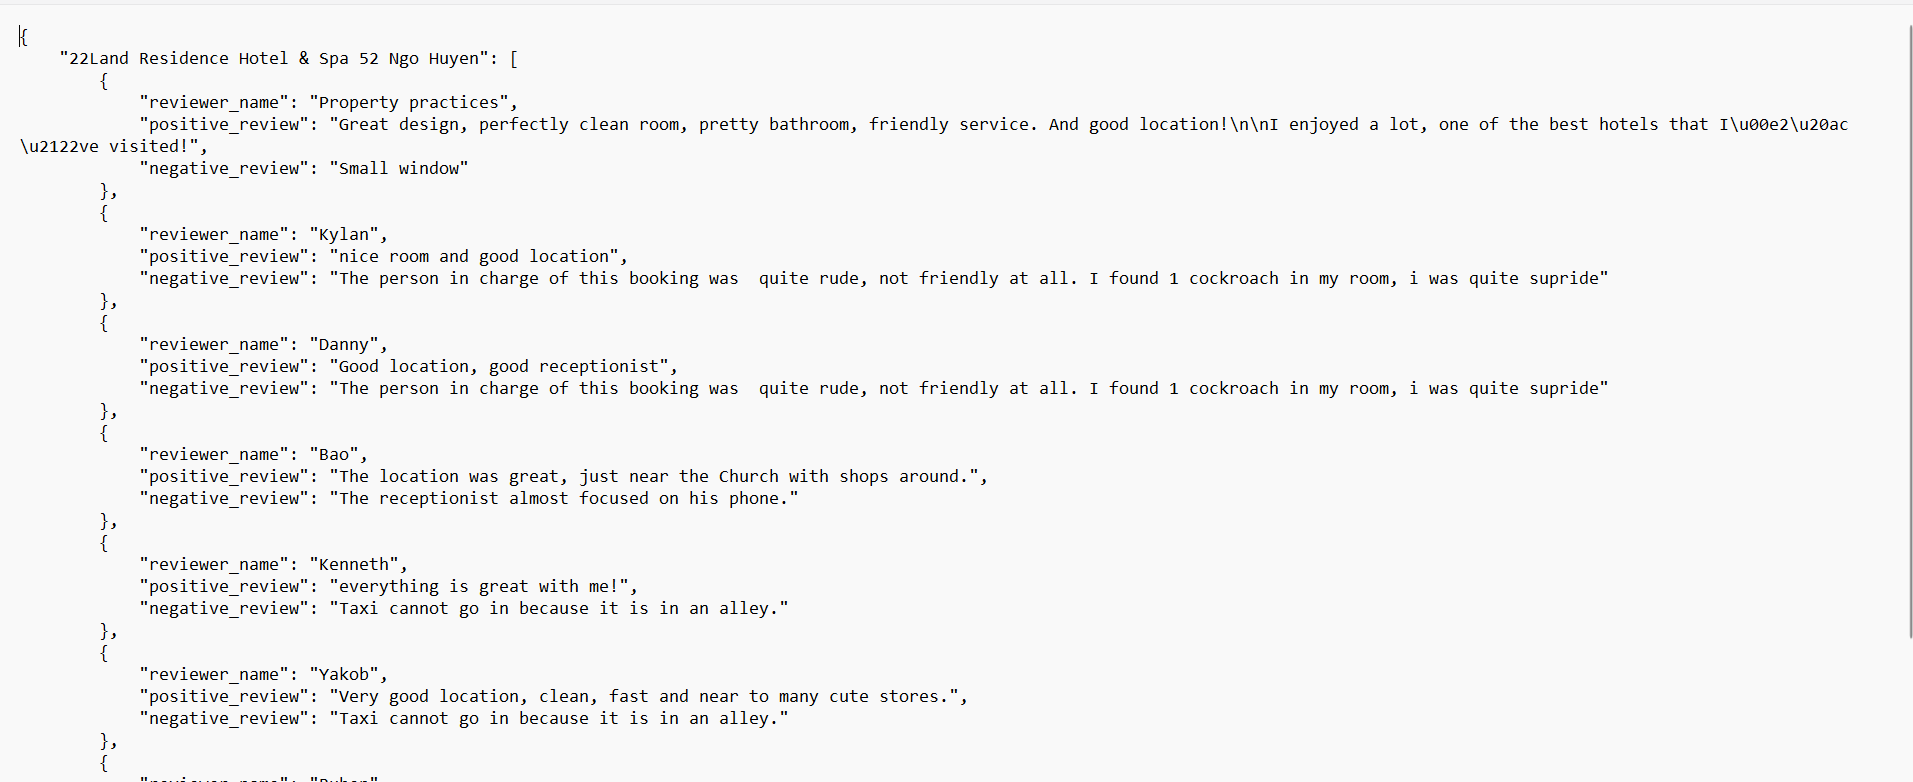
\includegraphics[width=1.0\linewidth]{Figures/1.1.png}
        \caption{Tiến độ thực hiện thực tập}
        \label{fig:image}
        \end{figure}
        
        \item \textbf{Danh sách khách sạn ở Hà Nội} với đầy đủ thông tin về giá phòng, địa chỉ và điểm số chung để có thể dễ dàng đưa ra được khách sạn đáp ứng nhu cầu giá cả và gần địa điểm mong muốn.

        Đây là trang web động, sử dụng Selenium để có thể lấy được tên, địa chỉ và vị trí từng khách sạn ở Hà Nội trên trang web (HotelCrawl). Chi tiết hơn xem tại ảnh \hyperref[fig:image1.2]{Hình 2.3}
        
        \begin{figure} % Sử dụng [H]
        \centering
        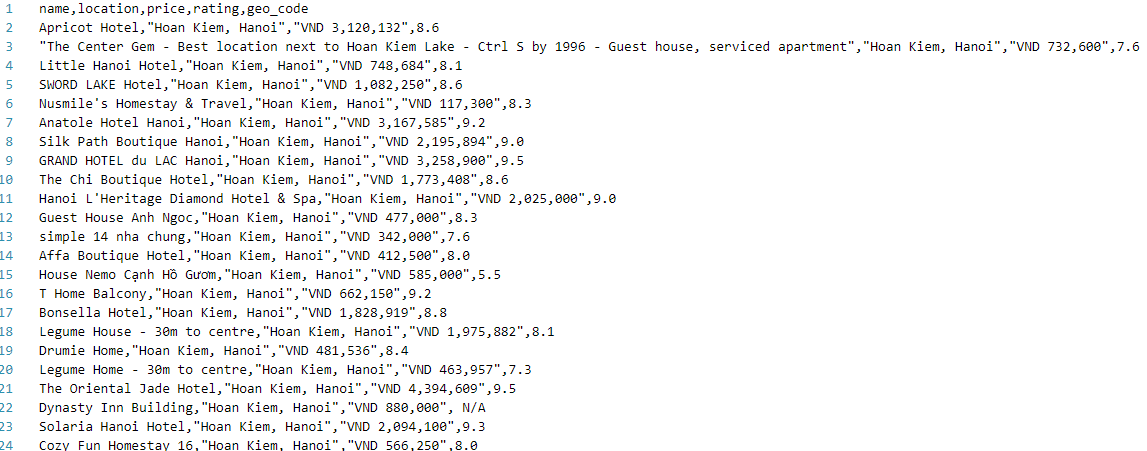
\includegraphics[width=1.0\linewidth]{Figures/1.22.png}
        \caption{Chú thích cho hình ảnh}
        \label{fig:image1.2}
        \end{figure}
        
    \end{enumerate}
    
    \item Xác định phương pháp thu thập
    \begin{enumerate}
        \item Sử dụng Selenium để tự động thu thập tên, địa chỉ và vị trí của từng khách sạn trên trang web. Sau đó, tiếp tục sử dụng Selenium để lấy các đánh giá tích cực và tiêu cực từ người dùng, nhằm xây dựng các đặc trưng riêng cho mỗi khách sạn.Chi tiết hơn xem tại ảnh \hyperref[fig:image2.4]{Hình 2.4}

        \begin{figure}[H] % Sử dụng [H]
        \centering
        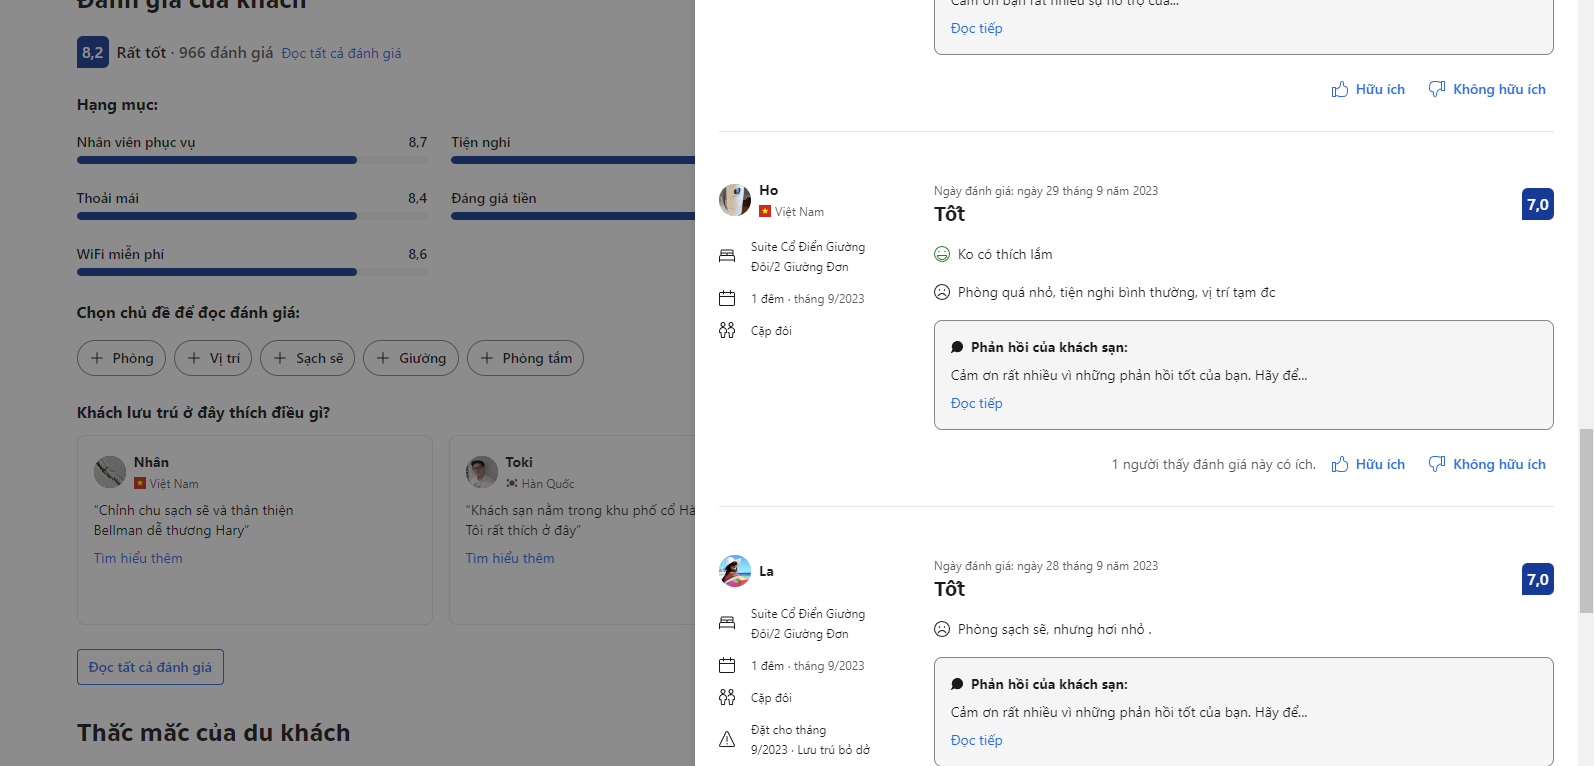
\includegraphics[width=1.0\linewidth]{Figures/1.3.png}
        \caption{Tiến độ thực hiện thực tập}
        \label{fig:image2.4}
        \end{figure}
        
        \item Sample khi thu được ở khách sạn 22Land Residence Hotel  Spa 52 Ngo Huyen:
        
        \begin{figure}[H] % Sử dụng [H]
        \centering
        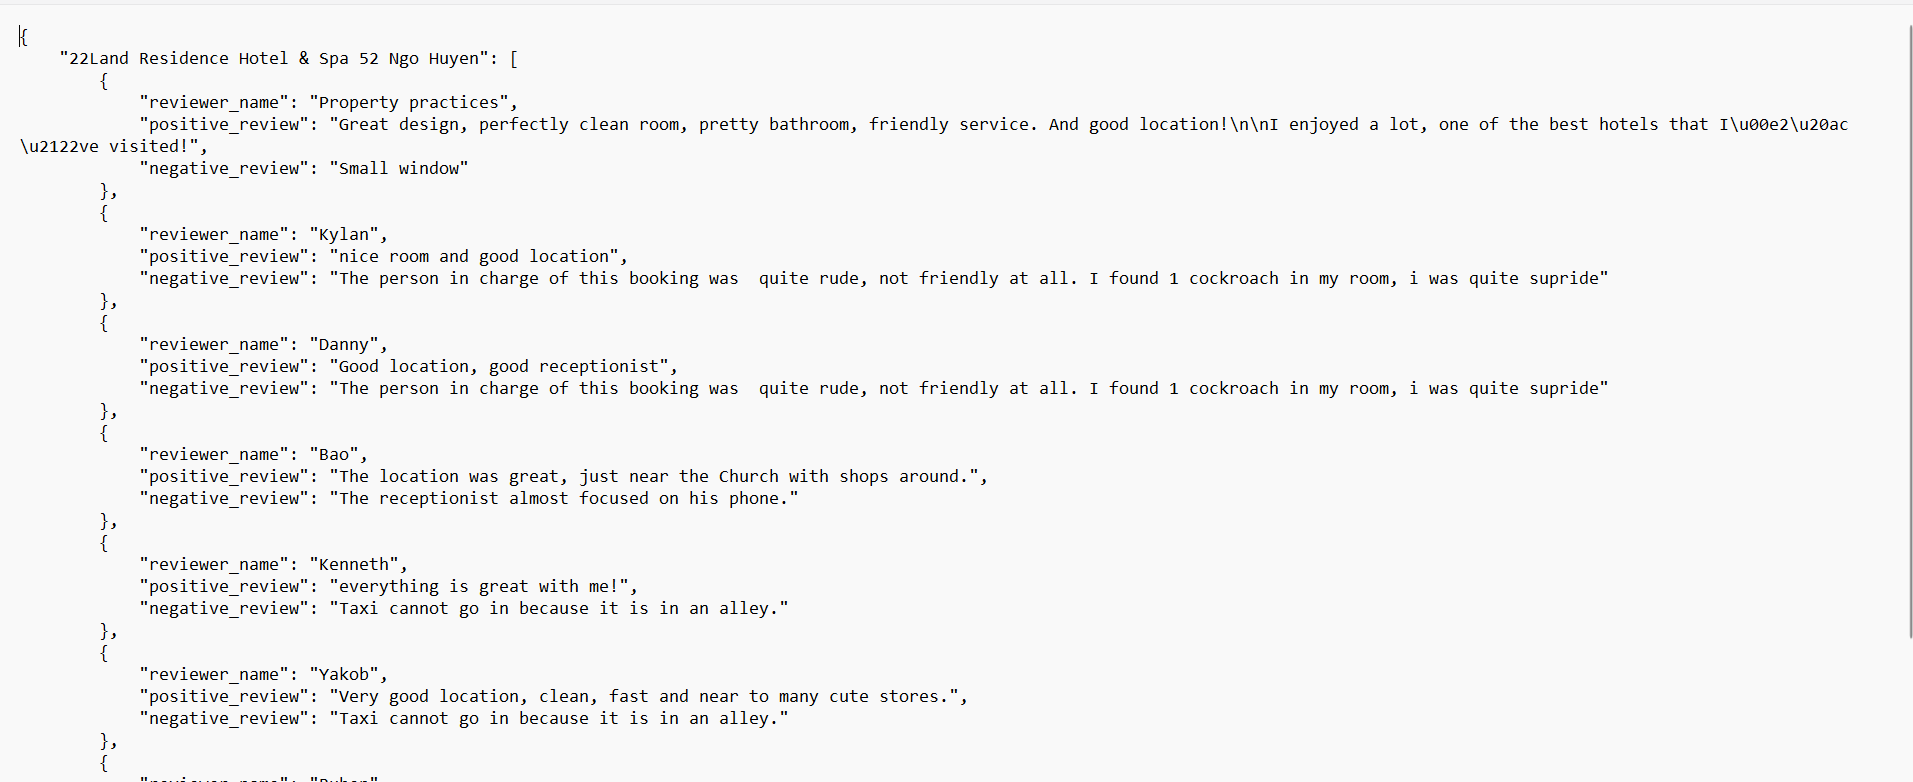
\includegraphics[width=1.0\linewidth]{Figures/1.4.png}
        \caption{Tiến độ thực hiện thực tập}
        \label{fig:iot}
        \end{figure}
        
    \end{enumerate}
\end{enumerate}


\textbf{Kết luận:} 

\section{Chủ đề tìm hiểu tuần 5: Làm sạch dữ liệu}

\subsection{Mục tiêu tuần 5}
Mục tiêu của tuần này là làm sạch và chuẩn bị dữ liệu cho hệ thống gợi ý khách sạn, đảm bảo dữ liệu đầu vào chính xác và đầy đủ để mô hình hoạt động hiệu quả.

\subsection{Kết quả tuần 5}

\subsubsection{Xử lý dữ liệu từ file \texttt{HotelName.csv}}
\begin{itemize}
    \item \textbf{Thông tin dữ liệu:} Dữ liệu từ file CSV chứa các thông tin quan trọng về khách sạn tại Hà Nội, bao gồm tên khách sạn, địa chỉ, giá phòng và điểm số trung bình.  Xem thêm thông tin chi tiết tại \hyperlink{fig:iot123}{ảnh}. 
    \begin{figure} % Sử dụng [H]
        \centering
        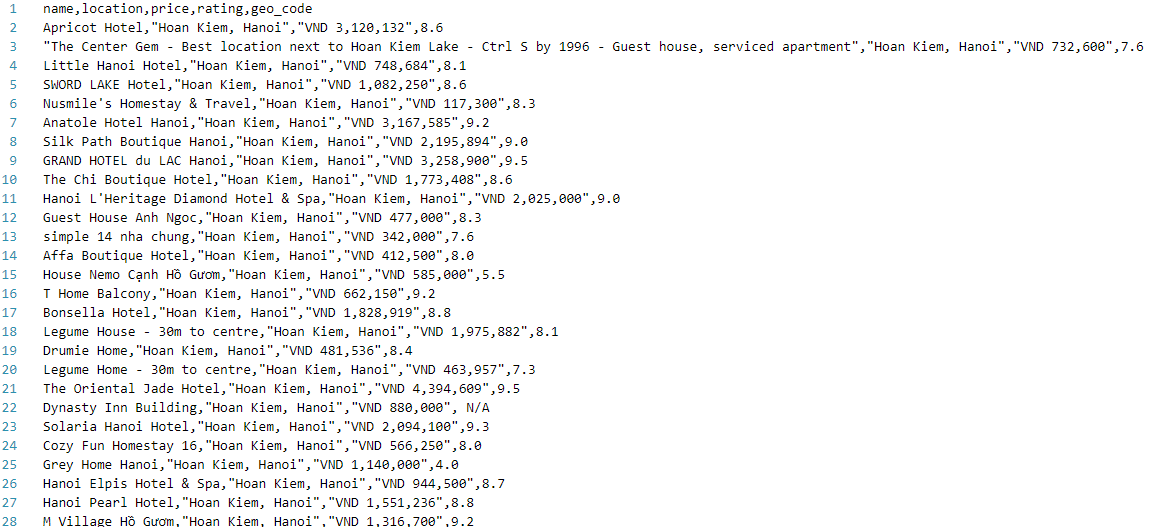
\includegraphics[width=1.0\linewidth]{Figures/2.1.1.png}
        \caption{Thông tín dữ liệu khách sạn}
        \label{fig:iot123}
    \end{figure}
    \item \textbf{Kiểm tra dữ liệu:} Trong quá trình thu thập dữ liệu, có thể xảy ra tình trạng dữ liệu bị thiếu hoặc không chính xác. lập trình viên đã thực hiện kiểm tra để xác nhận rằng không có khách sạn nào bị thiếu nhãn địa chỉ.
    \begin{figure}[H] % Sử dụng [H]
        \centering
        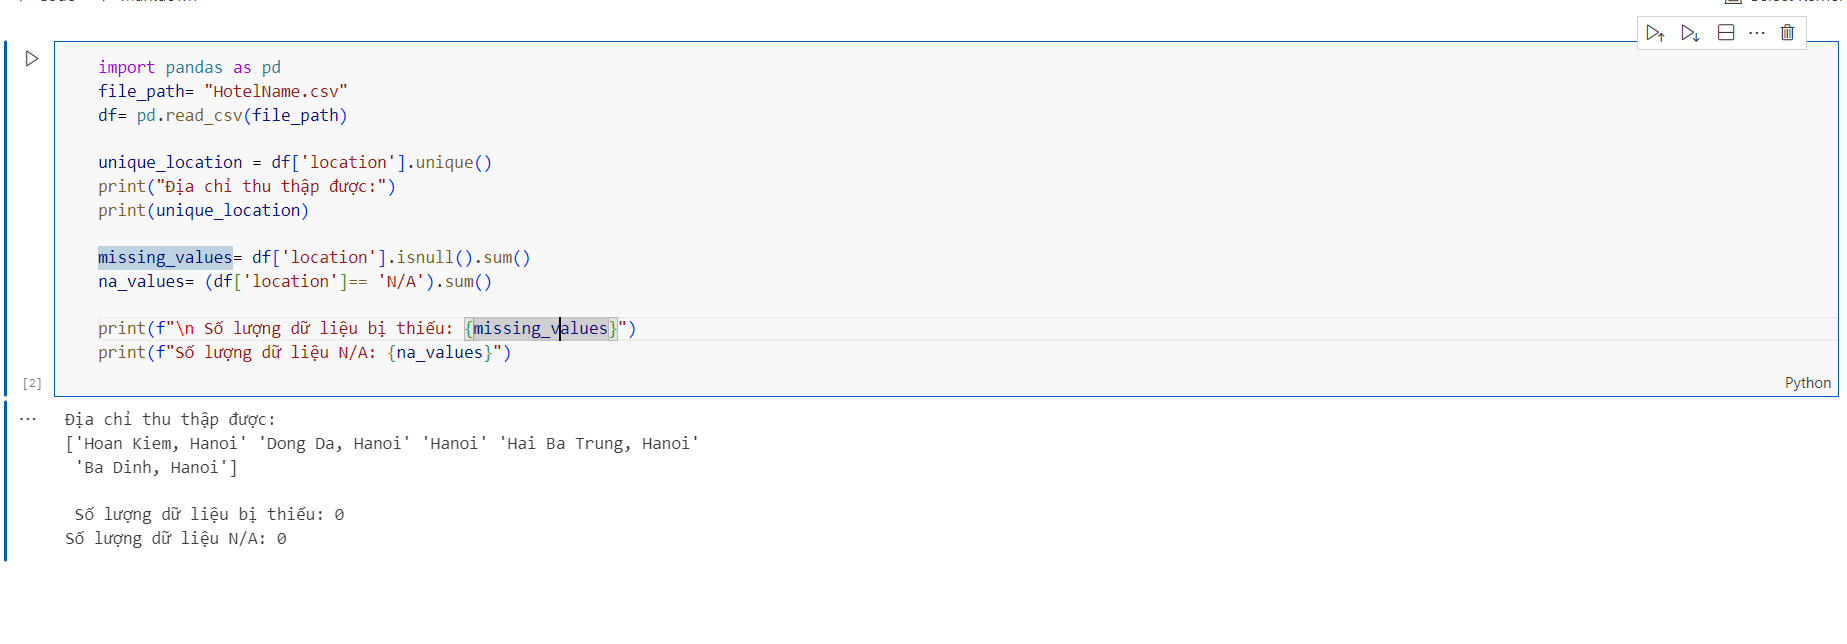
\includegraphics[width=1.0\linewidth]{Figures/2.2.png}
        \caption{Kết quả không có khách sạn nào bị mất nhãn địa chỉ}
        \label{fig:iot}
    \end{figure}
    
    Tiếp theo, lập trình viên sử dụng thư viện Matplotlib để trực quan hoá khách sạn theo từng địa điểm:
    \begin{figure}[H] % Sử dụng [H]
        \centering
        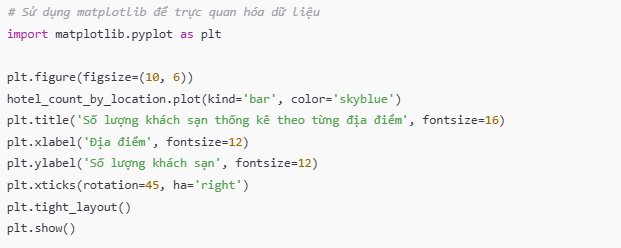
\includegraphics[width=1.0\linewidth]{Figures/2.3.1.png}
        \caption{Thư viện matplotlib}
        \label{fig:iot}
    \end{figure}
    \begin{figure}[H] % Sử dụng [H]
        \centering
        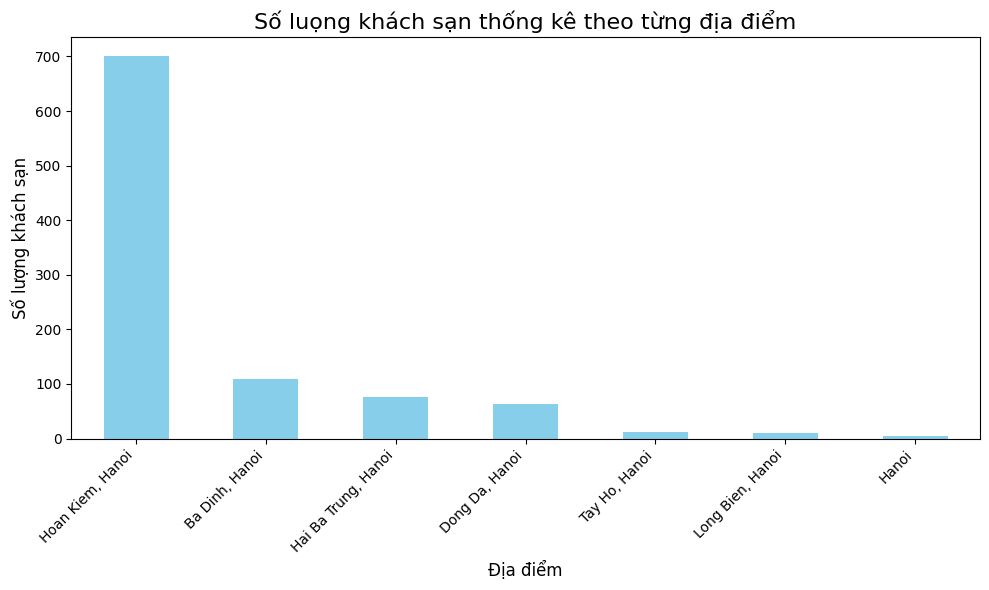
\includegraphics[width=1.0\linewidth]{Figures/2.4.png}
        \caption{biểu đồ lượng khách sạn trong các khu vực Hà Nội}
        \label{fig:iot}
    \end{figure}
    \item \textbf{Xử lý lỗi địa chỉ:} Một số địa chỉ trong dữ liệu bị ghi chung chung như “Hanoi”, điều này gây khó khăn trong việc xác định một cách chính xác vị trí. Vì thế lập trình viên đã thực hiện các bước sau để tiền xử lý lỗi địa chỉ:
    \begin{enumerate}
        \item Tìm và xác định các địa chỉ bị lỗi. 
        \begin{figure}[H] % Sử dụng [H]
        \centering
        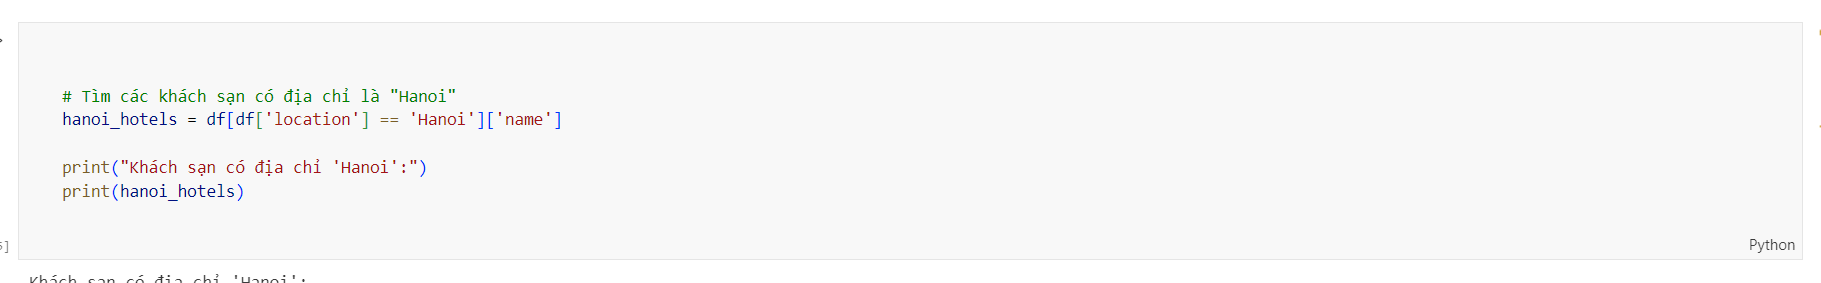
\includegraphics[width=1.0\linewidth]{Figures/2.5.png}
        \caption{Tìm địa chỉ lỗi}
        \label{fig:iot}
        \end{figure}
        
        \item Sử dụng Google để tìm kiếm và xác thực địa chỉ chính xác. 
        \begin{figure}[H] % Sử dụng [H]
        \centering
        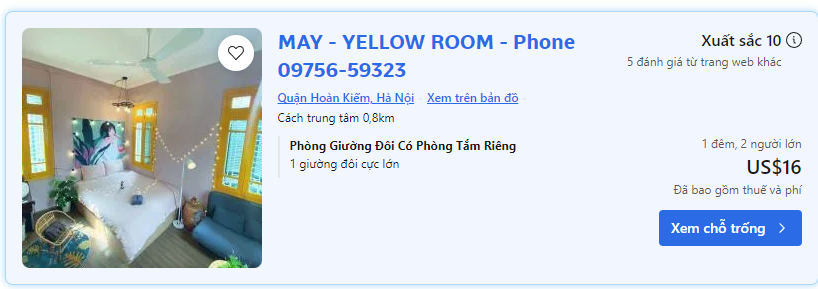
\includegraphics[width=0.8\linewidth]{Figures/2.6.png}
        \caption{Ví dụ khách sản sử dụng google để tìm kiếm}
        \label{fig:iot}
        \end{figure}
        Trước :
        \begin{figure}[H] % Sử dụng [H]
        \centering
        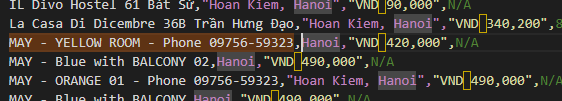
\includegraphics[width=1.0\linewidth]{Figures/2.7.png}
        \caption{Dữ liệu trước}
        \label{fig:iot}
        \end{figure}
        Sau:
        \begin{figure}[H] % Sử dụng [H]
        \centering
        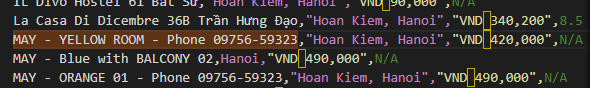
\includegraphics[width=1.0\linewidth]{Figures/2.8.png}
        \caption{Dự liệu sau khi sửa và cập nhập}
        \label{fig:iot}
        \end{figure}
        \item Sửa chữa và cập nhật địa chỉ trong dữ liệu.
        \begin{figure}[H] % Sử dụng [H]
        \centering
        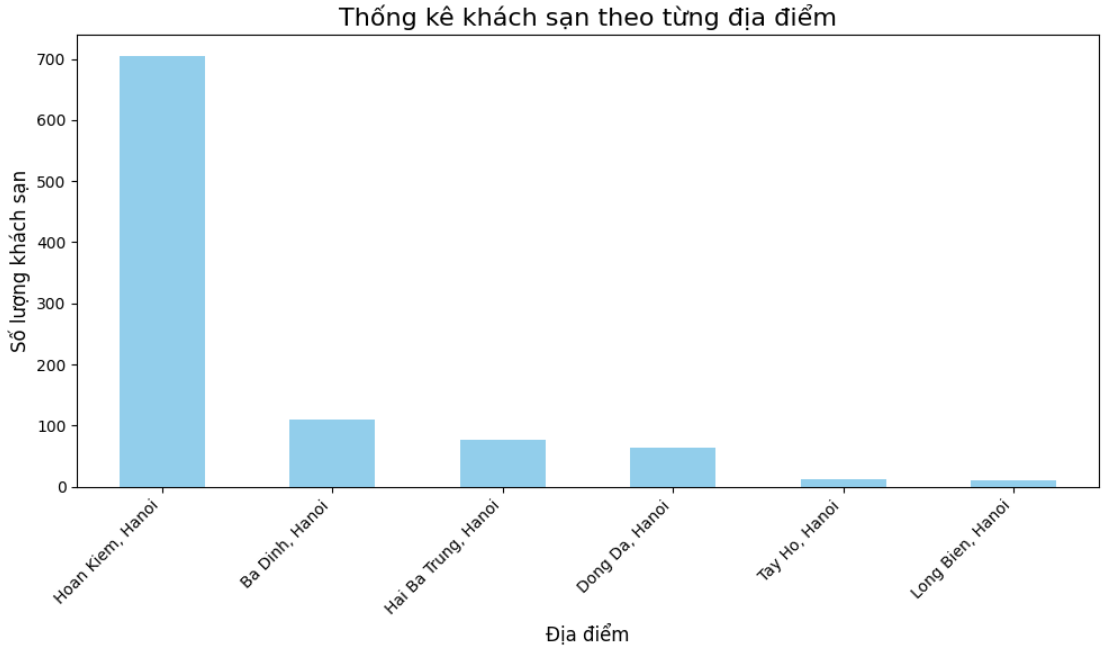
\includegraphics[width=1.0\linewidth]{Figures/2.9.png}
        \label{fig:iot}
    \end{figure}
    \end{enumerate}
    
    \item \textbf{Chuyển đổi địa chỉ thành tọa độ địa lý:} Để hệ thống có thể hiểu và xử lý vị trí của các khách sạn, lập trình viên đã sử dụng dịch vụ geocoding Nominatim để chuyển đổi địa chỉ thành tọa độ địa lý. Dịch vụ này cho phép chuyển đổi từ địa chỉ văn bản sang tọa độ chính xác. 
    \begin{figure}[H] % Sử dụng [H]
        \centering
        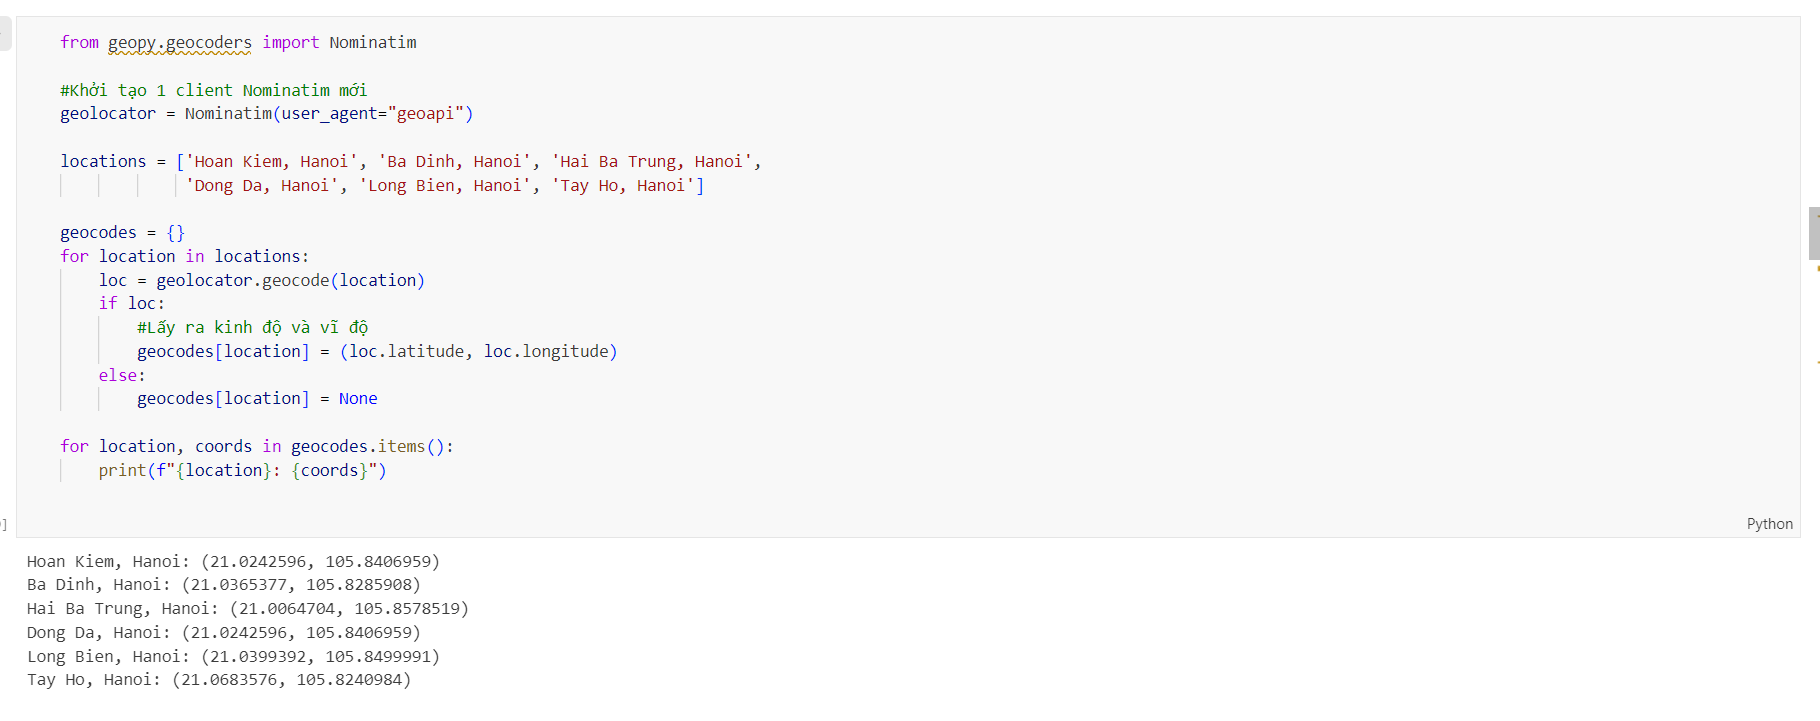
\includegraphics[width=1.0\linewidth]{Figures/2.10.png}
        \caption{Hàm chuyển tọa độ địa chỉ về tọa độ địa lý}
        \label{fig:iot}
    \end{figure}
    
    \item \textbf{Trực quan hóa dữ liệu trên bản đồ:} lập trình viên đã sử dụng thư viện Folium để trực quan hóa các vị trí của khách sạn trên bản đồ, giúp dễ dàng phân tích và theo dõi các khu vực.
    \begin{figure}[H] % Sử dụng [H]
        \centering
        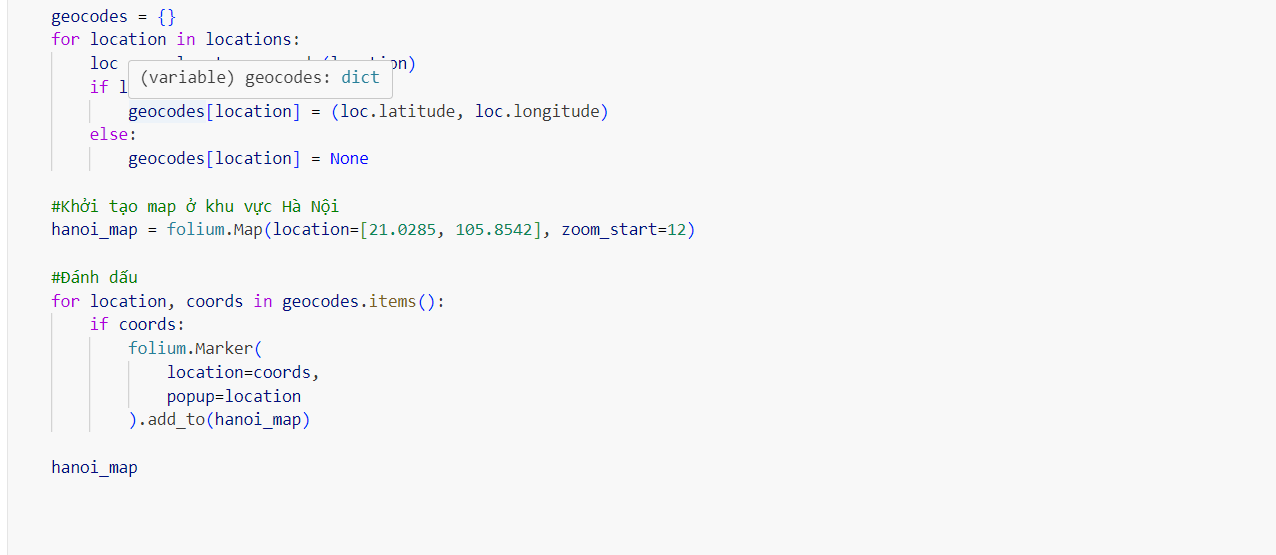
\includegraphics[width=1.0\linewidth]{Figures/2.11.png}
        \caption{Thư viện folium}
        \label{fig:iot}
    \end{figure}
    \begin{figure}[H] % Sử dụng [H]
        \centering
        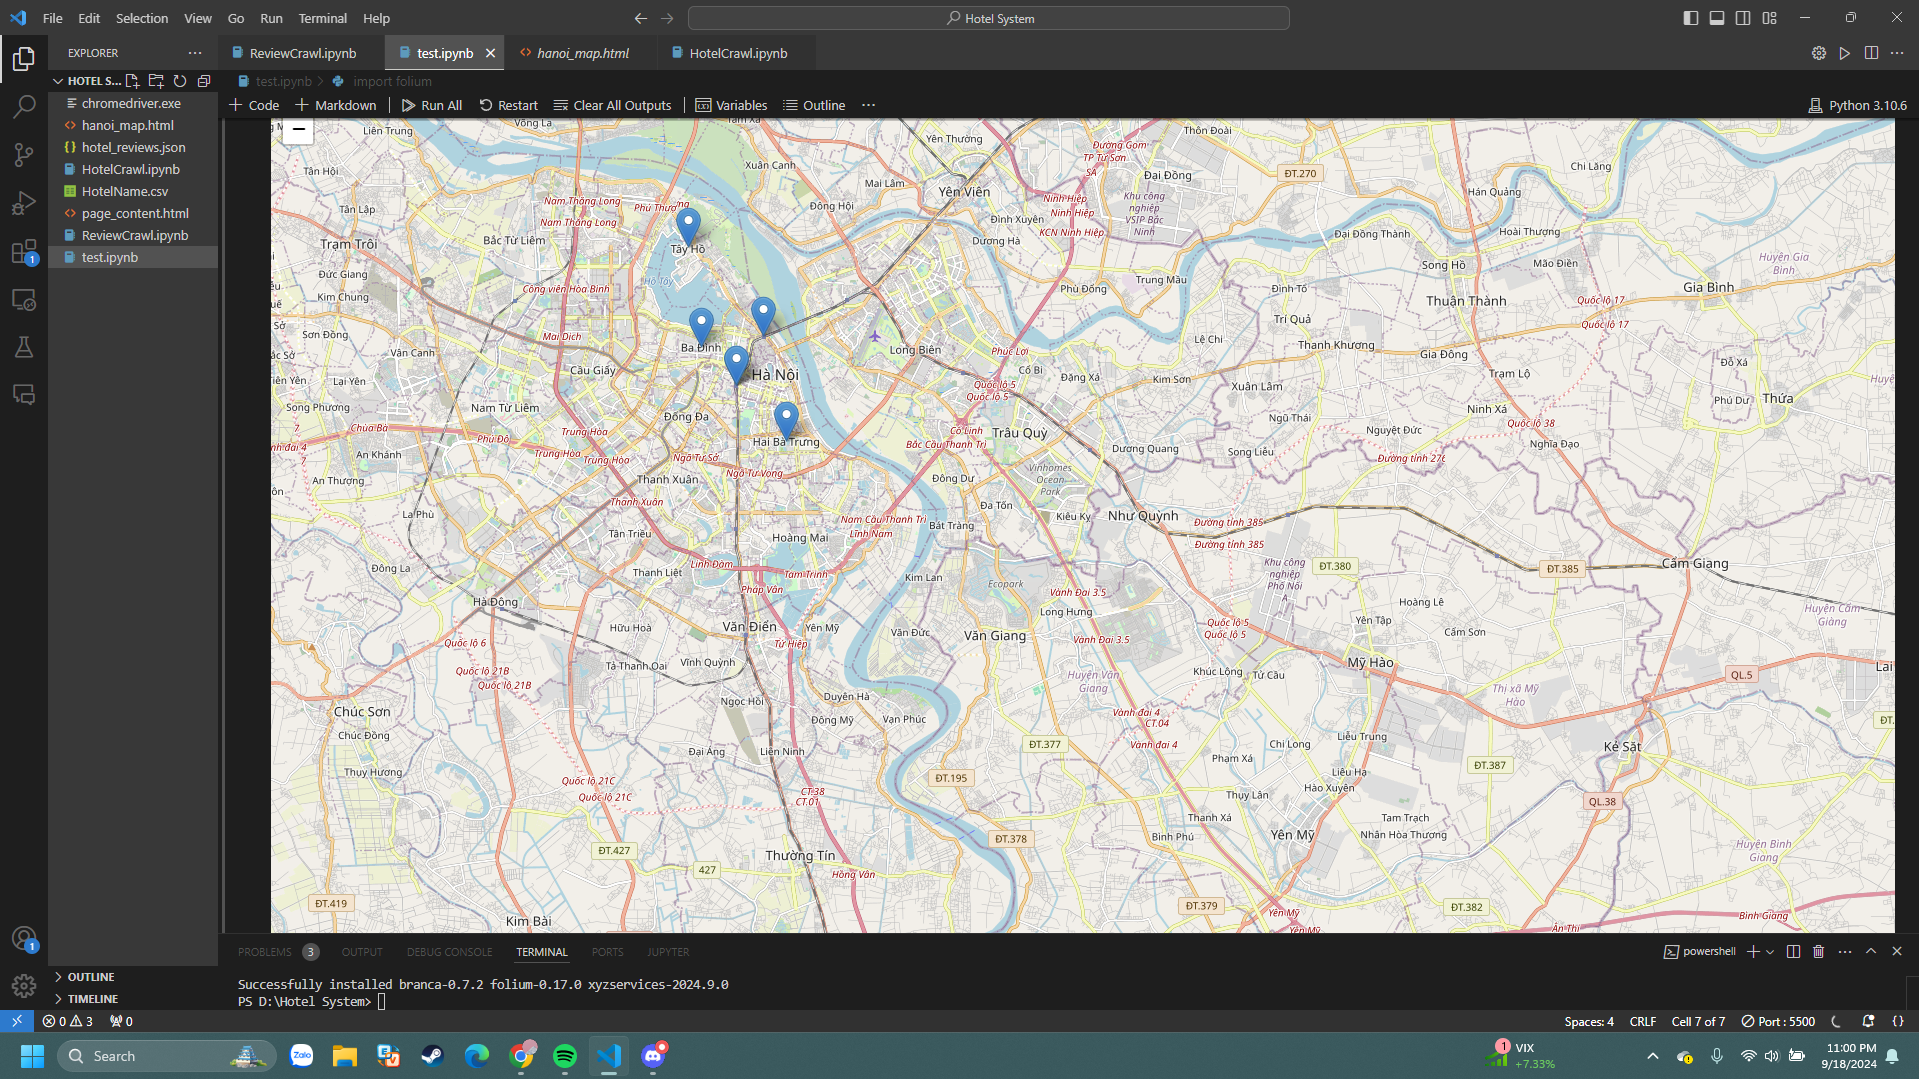
\includegraphics[width=1.0\linewidth]{Figures/2.12.png}
        \caption{Các khách sạn hiển thị trên bản đồ địa lý}
        \label{fig:iot}
    \end{figure}
    \begin{figure}[H] % Sử dụng [H]
        \centering
        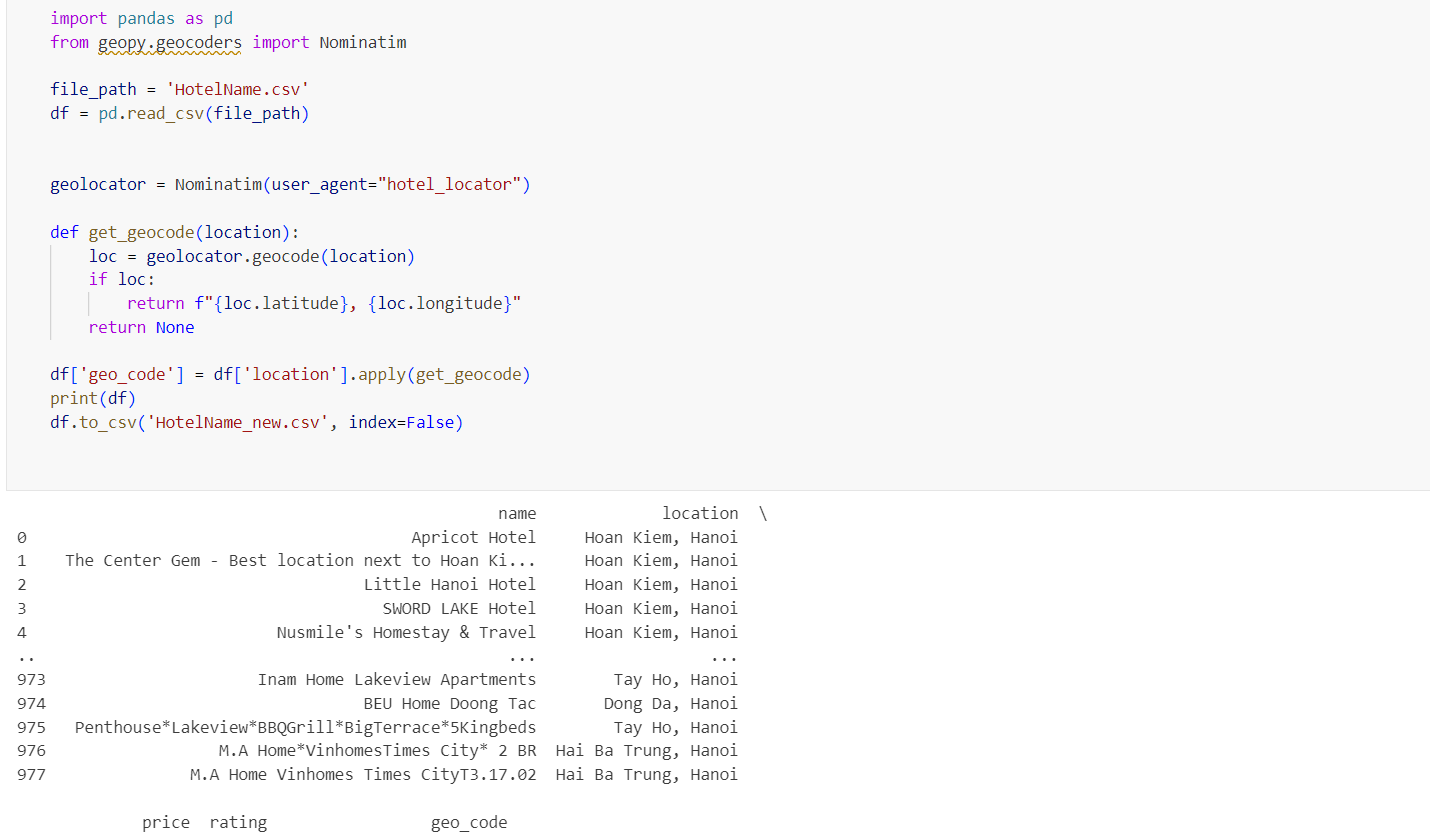
\includegraphics[width=1.0\linewidth]{Figures/2.13.png}
        \caption{Hàm xử lí}
        \label{fig:iot}
    \end{figure}
    \begin{figure}[H] % Sử dụng [H]
        \centering
        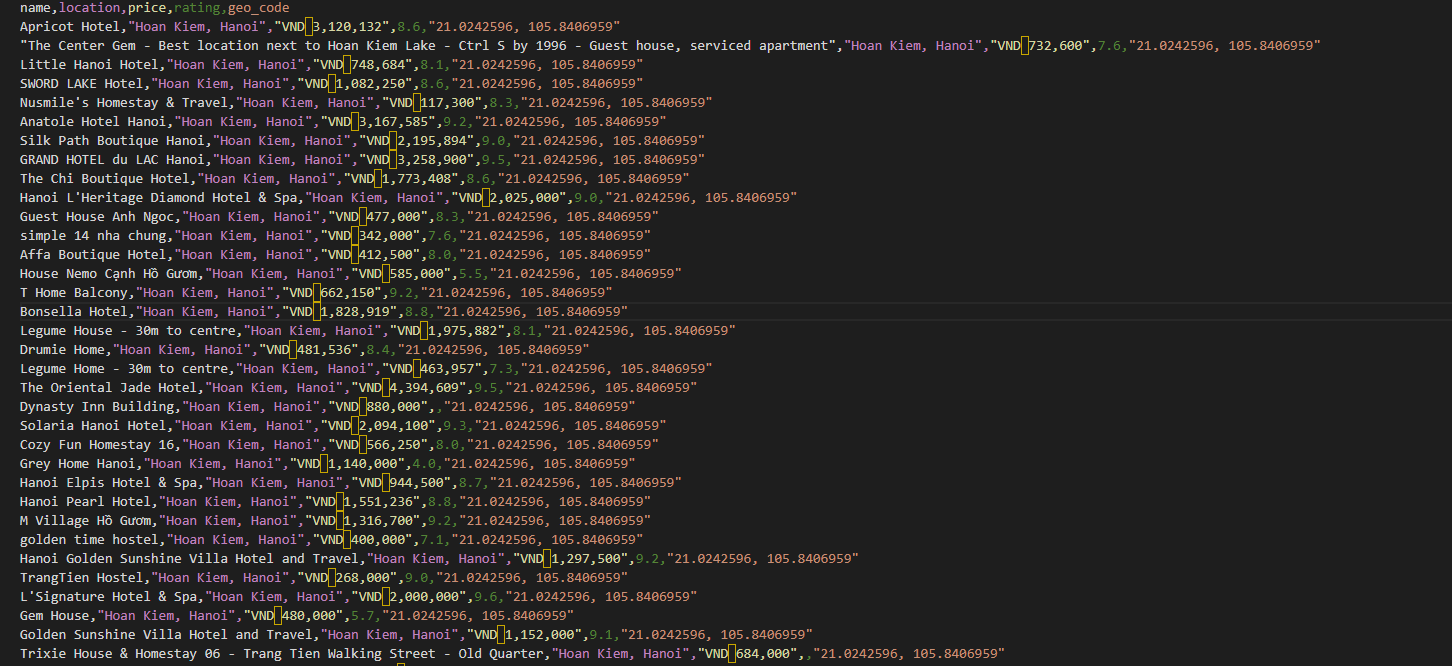
\includegraphics[width=1.0\linewidth]{Figures/2.14.png}
        \caption{Dự liệu csv các khách sạn thu thập được}
        \label{fig:iot}
    \end{figure}
\end{itemize}

\subsubsection{Xử lý giá phòng}
\begin{itemize}
    \item \textbf{Chuẩn hóa giá phòng:} Giá phòng thu thập được đã được chuẩn hóa về cùng một mệnh giá (VND) để đảm bảo tính nhất quán trong dữ liệu.
    \begin{figure}[H] % Sử dụng [H]
        \centering
        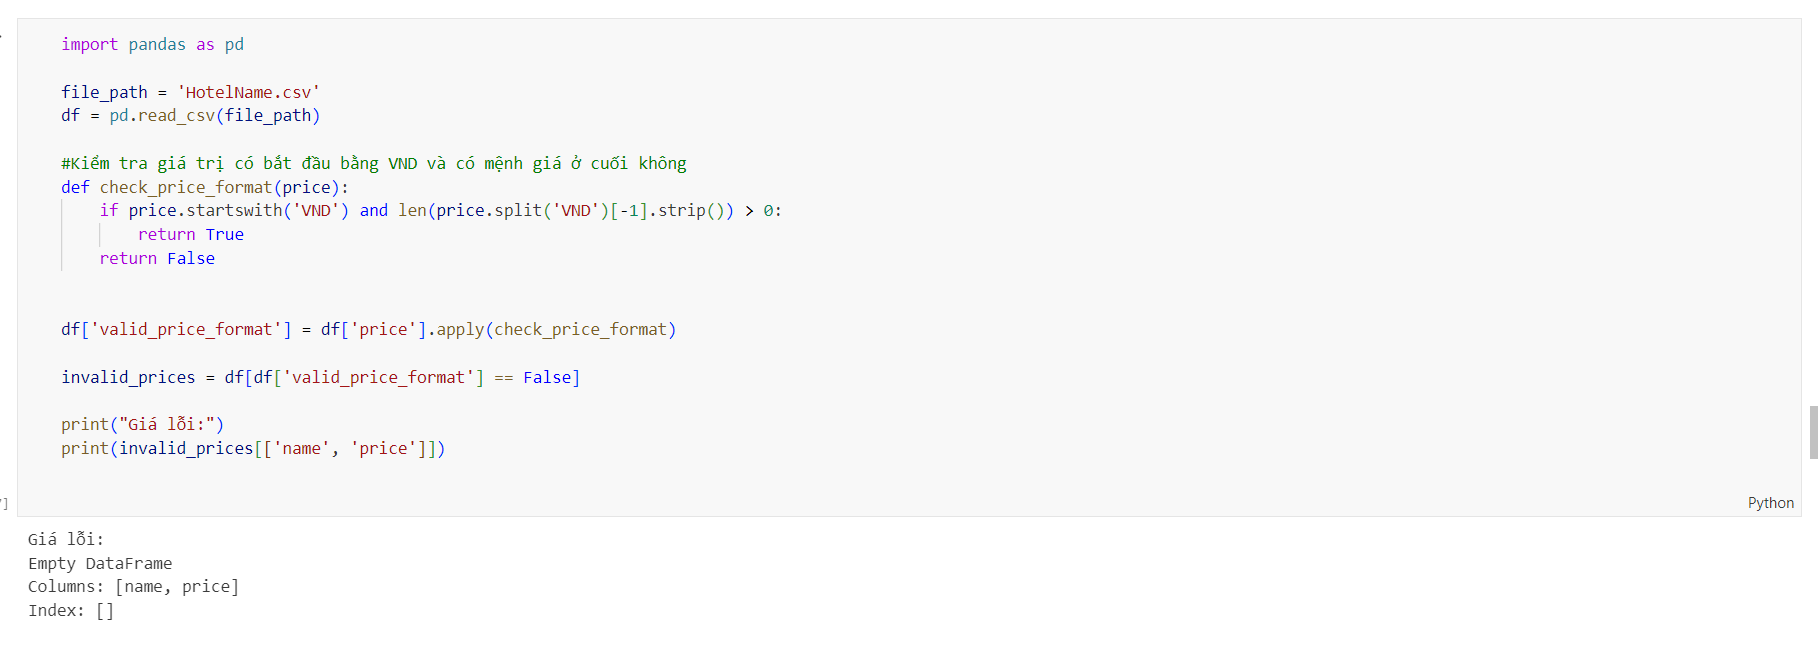
\includegraphics[width=0.8\linewidth]{Figures/2.15.png}
        \caption{Hàm chuẩn hóa}
        \label{fig:iot}
    \end{figure}
\end{itemize}

\subsubsection{Xử lý điểm đánh giá}
\begin{itemize}
    \item \textbf{Dữ liệu điểm đánh giá:} Một số khách sạn có dữ liệu điểm đánh giá bị thiếu (N/A). Tỷ lệ khách sạn bị thiếu điểm đánh giá là 147/978. 
    \begin{figure}[H] % Sử dụng [H]
        \centering
        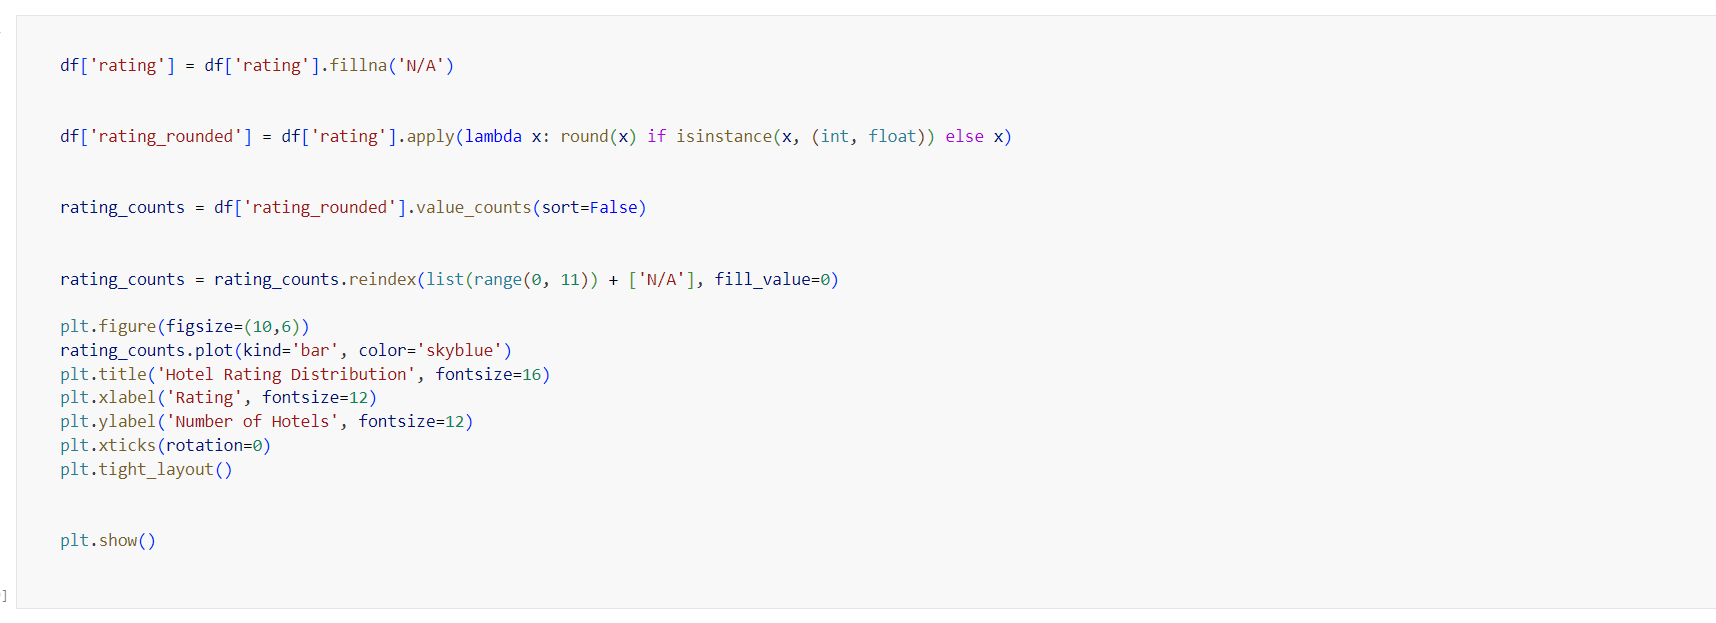
\includegraphics[width=1.0\linewidth]{Figures/2.16.png}
        \caption{hàm xử lý điểm đánh giá}
        \label{fig:iot}
    \end{figure}
    \begin{figure}[H] % Sử dụng [H]
        \centering
        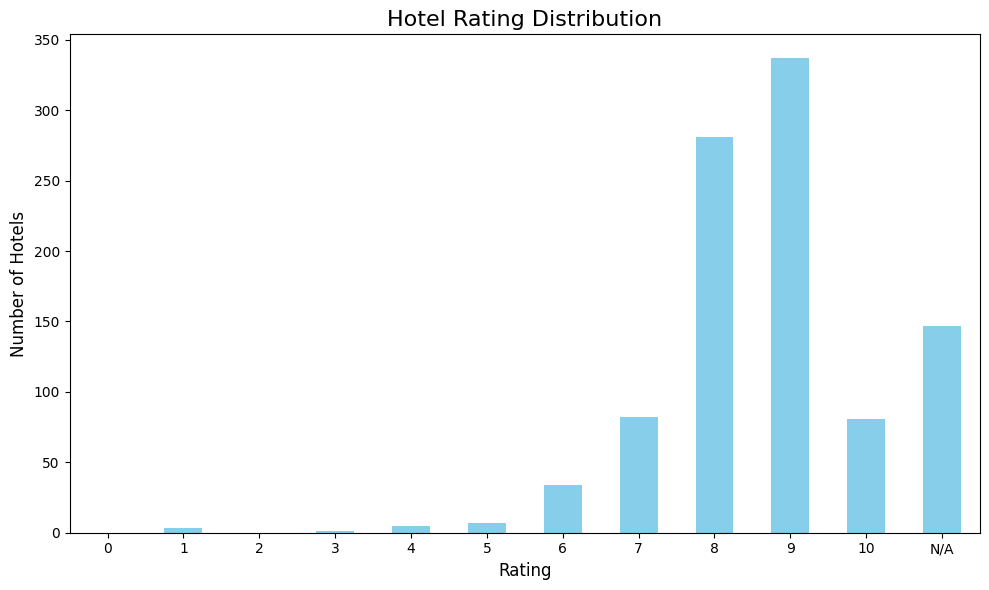
\includegraphics[width=1.0\linewidth]{Figures/2.17.png}
        \caption{Biểu đồ rating của khách sản}
        \label{fig:iot}
    \end{figure}
    Có thể thấy số lượng khách sạn bị “N/A” trong quá trình dữ liệu khá lớn: Chi tiết hơn xem tại ảnh \hyperref[fig:image2.22]{Hình 2.22}
     \begin{figure} [h] % Sử dụng [H]
        \centering
        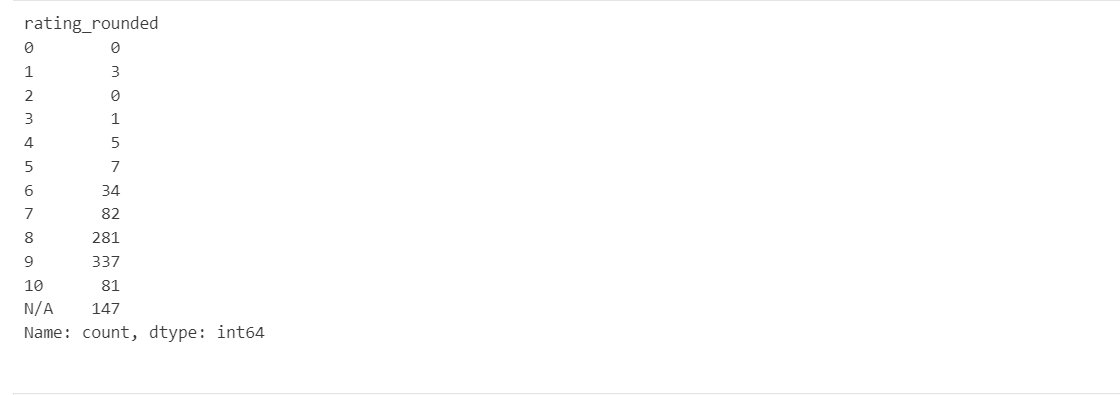
\includegraphics[width=1.0\linewidth]{Figures/2.18.png}
        \caption{Ví dụ}
        \label{fig:image2.22}
    \end{figure}
    \item \textbf{Phương án xử lý:} 
    \begin{enumerate}
        \item Tìm kiếm và bổ sung điểm đánh giá thủ công từ các nguồn khác.
        \item Sử dụng điểm đánh giá từ các trang đánh giá khách sạn khác như TripAdvisor để thay thế.
        \item Nếu không thể tìm thấy thông tin, phân phối điểm số trung bình (ví dụ, 6 điểm).
    \end{enumerate}
\end{itemize}

\subsubsection{Xử lý review của từng khách sạn}
\begin{itemize}
    \item \textbf{Dữ liệu review:} Bình luận của khách sạn được lưu dưới dạng file JSON. Một số review bị trùng lặp đã được phát hiện và loại bỏ. 
    \begin{figure}[H] % Sử dụng [H]
        \centering
        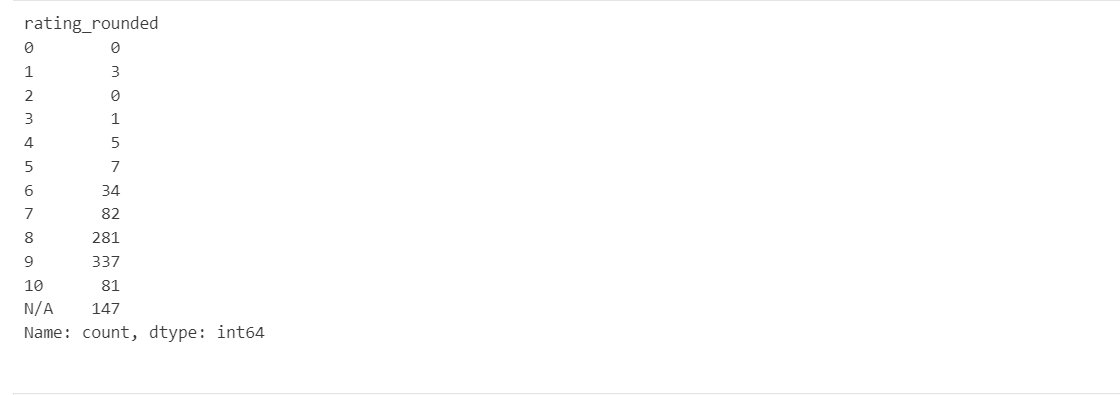
\includegraphics[width=1.0\linewidth]{Figures/2.18.png}
        \caption{Dữ liệu review được xử lý}
        \label{fig:iot}
    \end{figure}
    
    \item \textbf{Kết quả xử lý:} Sau khi loại bỏ các review trùng lặp, lập trình viên đã có các dữ liệu review sạch để mô hình học được đặc trưng của từng khách sạn. 
    \begin{figure}[H] % Sử dụng [H]
        \centering
        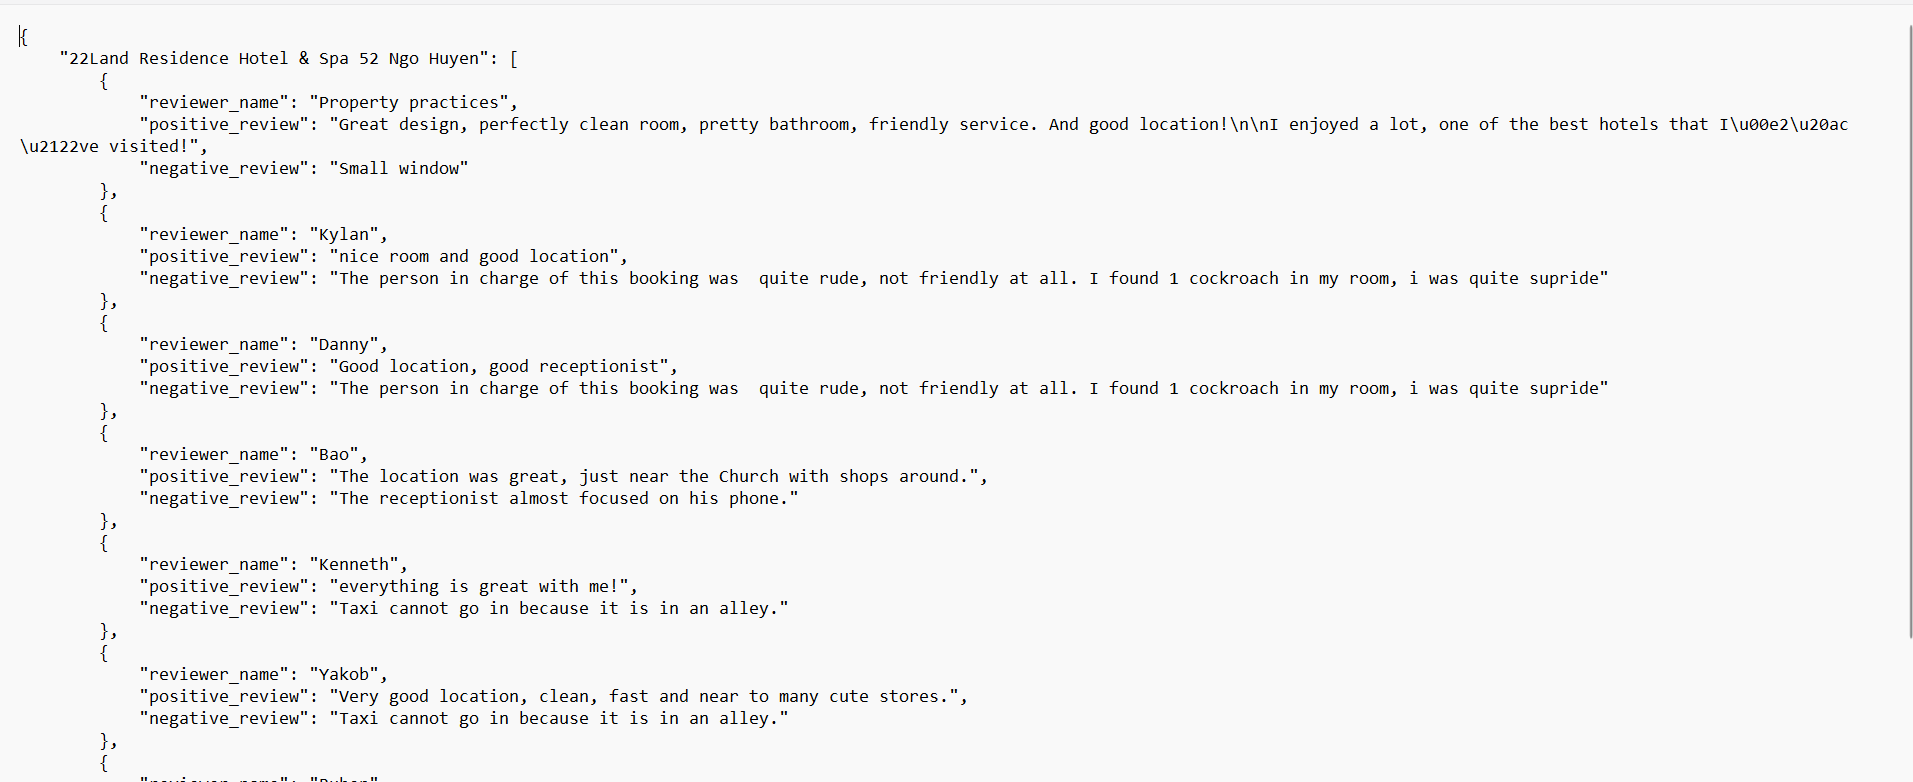
\includegraphics[width=1.0\linewidth]{Figures/2.19.png}
        \caption{Kết quả dự liệu sạch}
        \label{fig:iot}
    \end{figure}
    Kết quả thu nhập được :
    \begin{figure}[H] % Sử dụng [H]
        \centering
        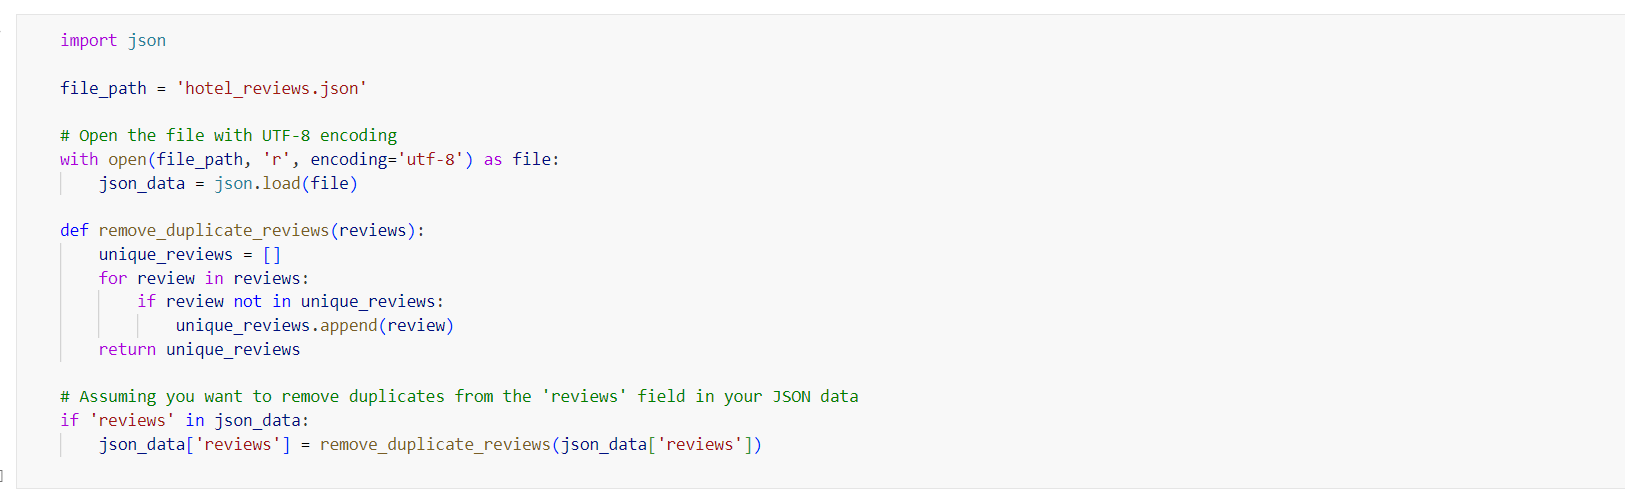
\includegraphics[width=1.0\linewidth]{Figures/2.20.png}
        \caption{Hàm thu thập}
        \label{fig:iot}
    \end{figure}
    \item \textbf{Tạo đặc trưng từ review:} Các review tích cực và tiêu cực đã được nối lại để mô hình học được ưu điểm và nhược điểm của từng khách sạn.Chi tiết hơn xem tại ảnh \hyperref[fig:image2.26]{Hình 2.26}
    \begin{figure}[H] % Sử dụng [H]
        \centering
        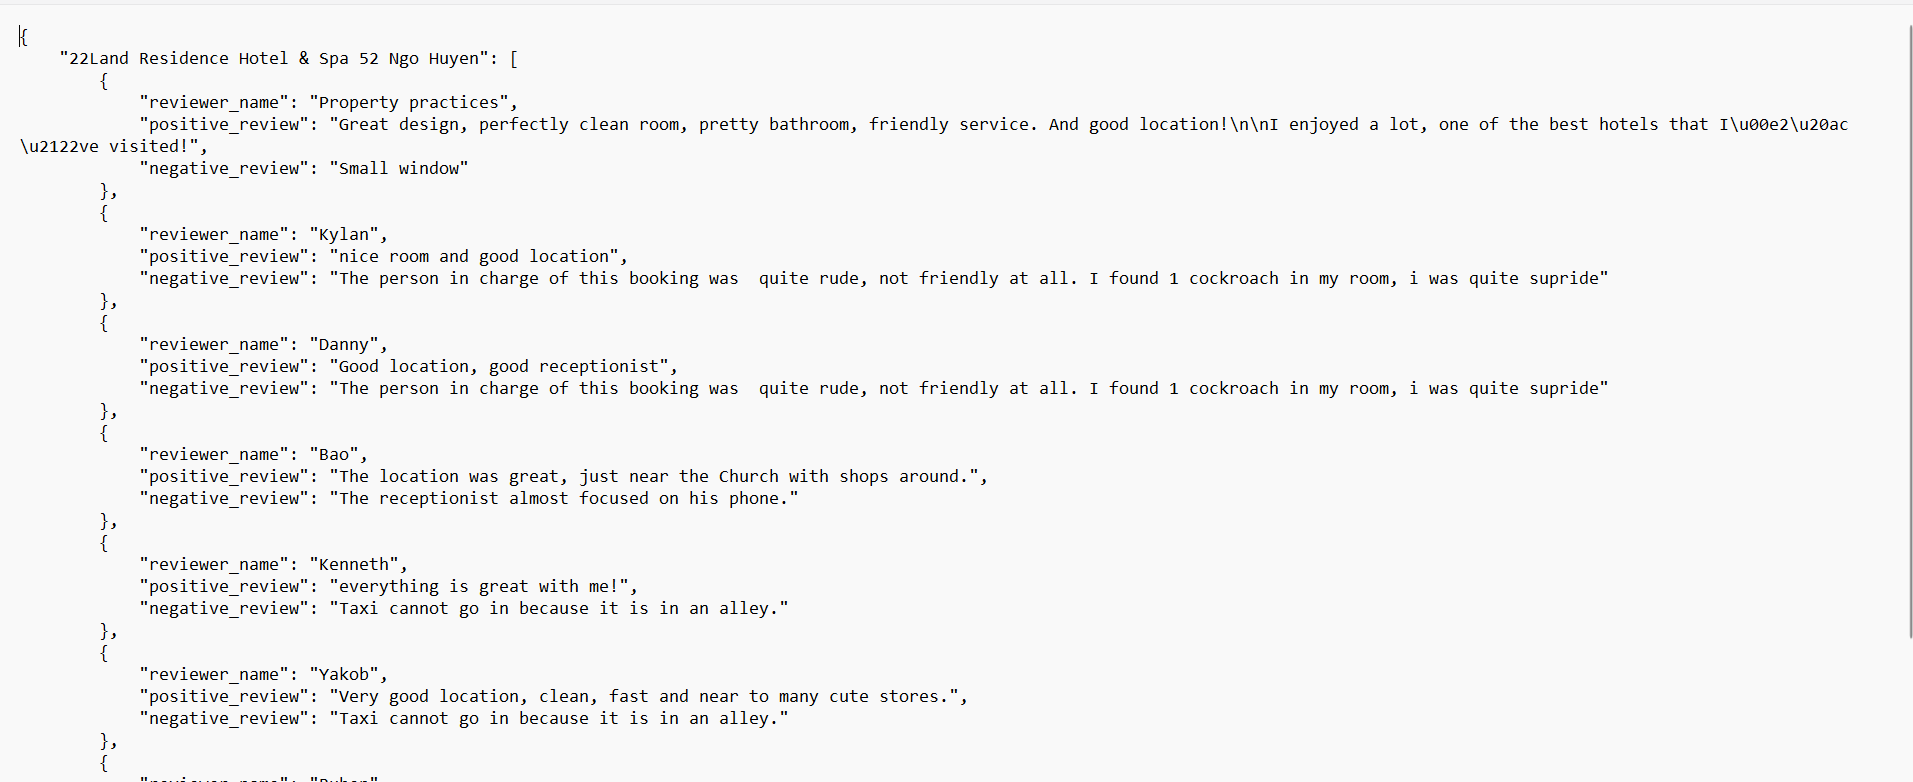
\includegraphics[width=1.0\linewidth]{Figures/2.21.png}
        \caption{Dữ liệu đã được xử lý}
        \label{fig:image2.26}
    \end{figure}
\end{itemize}

\textbf{Kết luận:} lập trình viên đã hoàn thành việc làm sạch dữ liệu và chuẩn bị đầy đủ các feature cần thiết cho mô hình đánh giá khách sạn, sẵn sàng cho các bước tiếp theo trong quy trình phát triển hệ thống.

\section{Chủ đề tìm hiểu tuần 6: Học máy}
\subsection{Mục tiêu tuần 6}
\setcounter{figure}{0} 
\renewcommand{\thefigure}{3.\arabic{figure}}
Tìm hiểu mô hình học máy. Mô hình Bert sử dụng các công nghệ xử lý ngôn ngữ tự nhiên để phân tích và trả lời các yêu cầu từ người dùng dựa trên review của khách hàng trước đó. Mục tiêu là giúp người dùng tìm kiếm các khách sạn phù hợp với các tiêu chí cụ thể mà họ đưa ra, như giá cả, dịch vụ, và các yếu tố khác từ những ưu điểm và nhược điểm được trích xuất từ các đánh giá.

\subsection{Mô hình BERT}
 \textbf{Giới thiệu mô hình BERT :} BERT (Bidirectional Encoder Representations from Transformers) là một mô hình ngôn ngữ dựa trên kiến trúc Transformer, được phát triển bởi Google vào năm 2018. Điểm đặc biệt của BERT so với các mô hình trước đó là khả năng học các biểu diễn ngôn ngữ theo cả hai chiều (trái sang phải và phải sang trái), giúp mô hình hiểu rõ ngữ cảnh hơn. Đây là mô hình pre-trained (được huấn luyện trước) và có thể fine-tuned cho nhiều tác vụ khác nhau như dịch máy, phân loại văn bản, trả lời câu hỏi, v.v.
    
\textbf{Kiến trúc mô hình :} Transformer Encoder: BERT sử dụng phần mã hóa (encoder) của kiến trúc Transformer, dựa trên các lớp attention để học các mối quan hệ giữa các từ trong câu. BERT có thể học được ngữ cảnh của từ dựa trên cả phía trước và phía sau nó, không giống như các mô hình unidirectional trước đó chỉ nhìn từ một phía. Chi tiết hơn xem tại ảnh \hyperref[fig:image3.1]{Hình 3.1}
\begin{figure}[H] % Sử dụng [H]
        \centering
        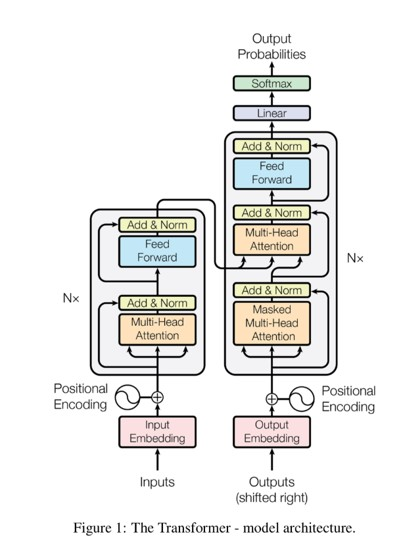
\includegraphics[width=0.8\linewidth]{Figures/bert1.jpg}
        \caption{Cấu trúc mô hình BERT}
        \label{fig:image3.1}
    \end{figure}

Pre-training tasks: BERT được huấn luyện trên hai nhiệm vụ chính:
\begin{itemize}
    \item \textbf{Masked Language Model (MLM):} Một số từ trong câu sẽ bị che đi, và mô hình được yêu cầu dự đoán từ đó dựa trên ngữ cảnh.
    \begin{figure}[H] % Sử dụng [H]
        \centering
        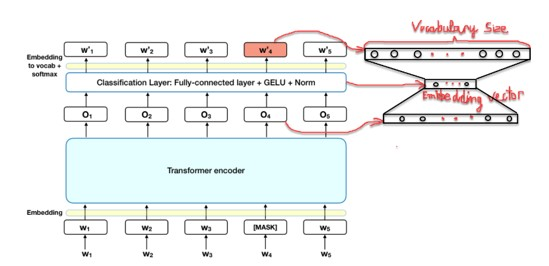
\includegraphics[width=0.6\linewidth]{Figures/bert2.jpg}
        \caption{Cấu trúc mô hình Masked Language Model}
        \label{fig:iot}
    \end{figure}

    \item \textbf{Next Sentence Prediction (NSP): } Mô hình được huấn luyện để dự đoán xem một câu có là câu tiếp theo trong đoạn văn hay không.
    \begin{figure}[H] % Sử dụng [H]
        \centering
        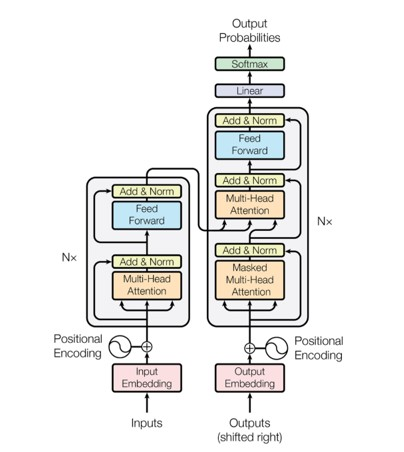
\includegraphics[width=0.6\linewidth]{Figures/bert3.jpg}
        \caption{Cấu trúc Next Sentence Prediction}
        \label{fig:iot}
    \end{figure}
    
\end{itemize}

Layers: BERT có các phiên bản nhỏ (BERT-Base) và lớn (BERT-Large). 

\textbf{Ví dụ:}  BERT-Base có 12 layers, 768 ẩn số, và 12 attention heads; 

 BERT-Large có 24 layers, 1024 ẩn số, và 16 attention heads


\textbf{Ưu và nhược điểm } 

\textbf{Ưu Điểm:}

\begin{itemize}
    \item Bi-directional context: BERT có thể hiểu được ngữ cảnh từ cả hai chiều, làm tăng độ chính xác trong nhiều bài toán xử lý ngôn ngữ tự nhiên (NLP).
    \item Transfer learning: BERT là một mô hình pre-trained, có thể fine-tune cho nhiều tác vụ khác nhau mà không cần huấn luyện từ đầu, tiết kiệm tài nguyên và thời gian.
    \item Hiệu suất cao: Trong nhiều bài toán như trả lời câu hỏi (QA) và phân loại văn bản, BERT thường đạt kết quả tốt hơn các mô hình trước đó.
\end{itemize}

\textbf{Nhược Điểm:}
\begin{itemize}
    \item Tốn tài nguyên: BERT yêu cầu nhiều tài nguyên tính toán (GPU/TPU) và thời gian huấn luyện, đặc biệt là các phiên bản lớn như BERT-Large.
    \item Chậm hơn trong inference: So với các mô hình đơn giản hơn, BERT có độ trễ cao hơn khi suy luận do số lượng lớn tham số và kiến trúc phức tạp.
    \item Overfitting với dữ liệu nhỏ: Khi fine-tune BERT trên các tập dữ liệu nhỏ, có thể dễ dàng bị overfitting nếu không cẩn thận trong quá trình huấn luyện.
\end{itemize}

\textbf{Ứng dụng }

\textbf{Hiểu yêu cầu người dùng:}

\begin{itemize}
    \item Người dùng nhập một câu truy vấn tự nhiên như: "Tôi đang ở HVBCVT, tôi muốn tìm khách sạn giá rẻ mà chất lượng vệ sinh ổn định."
    \item BERT Embedding được sử dụng để phân tích ngữ nghĩa của câu truy vấn, giúp mô hình hiểu được yêu cầu chính như: vị trí hiện tại của người dùng, loại khách sạn họ mong muốn (giá rẻ, vệ sinh tốt).
\end{itemize}

\textbf{Trích xuất thông tin quan trọng:}

\begin{itemize}
    \item Dựa trên kết quả embedding, mô hình có thể trích xuất các từ khóa quan trọng từ câu truy vấn. Ví dụ, “HVBCVT” được nhận diện là địa điểm (vị trí hiện tại của người dùng), còn “giá rẻ”, “vệ sinh ổn định” là tiêu chí lựa chọn khách sạn.
    \item Ngoài ra, BERT giúp xác định chính xác ngữ cảnh của các từ và cụm từ trong câu, như việc nhận biết rằng từ "HVBCVT" là một địa điểm thay vì một từ thông thường.
\end{itemize}

\textbf{Tích hợp tọa độ địa lý:}

\begin{itemize}
    \item Sau khi nhận diện địa điểm (HVBCVT), hệ thống sẽ sử dụng các API định vị (Geocoding) để tìm ra tọa độ chính xác của vị trí đó 
    \item Tiếp theo, danh sách các khách sạn có tọa độ địa lý sẵn có sẽ được lọc theo yêu cầu (như khách sạn trong khu vực Hà Đông, Thanh Xuân) và các tiêu chí về giá và chất lượng vệ sinh.
\end{itemize}

\textbf{Tính toán khoảng cách và gợi ý khách sạn:}

\begin{itemize}
    \item Với tọa độ của người dùng và các khách sạn, lập trình viên sử dụng các thuật toán tính toán khoảng cách để sắp xếp khách sạn dựa trên khoảng cách gần nhất với vị trí người dùng.
    \item Các tiêu chí về giá cả và chất lượng vệ sinh cũng được đánh giá song song, để đưa ra các gợi ý khách sạn phù hợp nhất.
\end{itemize}

\subsection{Cài Đặt}
\begin{itemize}
    \item \textbf{Cài đặt và import thư viện:} Cài đặt các công cụ và thư viện sau để bắt đầu xây dựng mô hình: Tensorflow, Transformers, Hugging Face, Gradio, Hugging Face Spaces
     \begin{figure}[H] % Sử dụng [H]
        \centering
        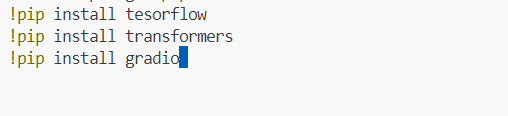
\includegraphics[width=0.6\linewidth]{Figures/hm1.jpg}
        \caption{Cài đặt thư viện}
        \label{fig:iot}
    \end{figure}



     \item \textbf{Tải mô hình và tokenizer:} Sử dụng mô hình đã huấn luyện sẵn từ Hugging Face để trích xuất các ưu điểm và nhược điểm từ review khách sạn.
    \begin{figure}[H] % Sử dụng [H]
        \centering
        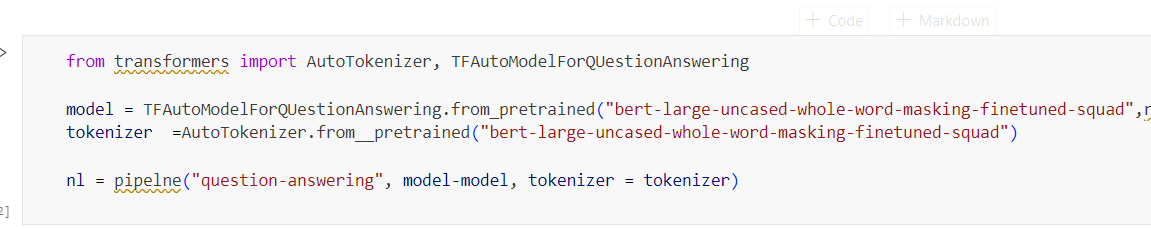
\includegraphics[width=1.3\linewidth]{Figures/hm2.png}
        \caption{Tải mô hình}
        \label{fig:iot}
    \end{figure}

         \item \textbf{Kiểm tra mô hình:} Chúng ta có thể kiểm tra mô hình bằng cách nhập vào các đoạn review khách sạn chứa thông tin về ưu và nhược điểm, sau đó đặt câu hỏi để tìm khách sạn phù hợp.
    \begin{figure}[H] % Sử dụng [H]
        \centering
        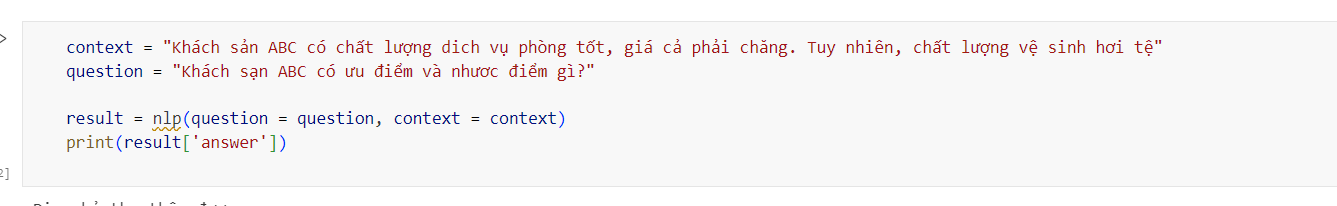
\includegraphics[width=1.3\linewidth]{Figures/hm3.png}
        \caption{Kiểm tra mô hình}
        \label{fig:iot}
    \end{figure}

      \item \textbf{Xây dựng mô hình chat Gợi ý Khách sạn:} Để ứng dụng vào hệ thống chat, chúng ta cần tạo một hàm xử lý yêu cầu của người dùng. Hàm này sẽ tìm ra khách sạn phù hợp dựa trên những tiêu chí mà người dùng cung cấp.
    \begin{figure}[H] % Sử dụng [H]
        \centering
        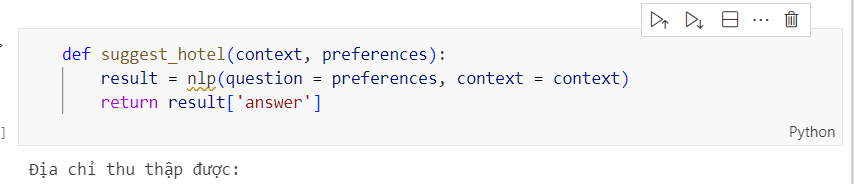
\includegraphics[width=1.0\linewidth]{Figures/hm4.png}
        \caption{Hàm xử lý}
        \label{fig:iot}
    \end{figure}

      \item \textbf{5. Khởi chạy ứng dụng} Khởi chạy ứng dụng để người dùng có thể thử nghiệm tìm kiếm khách sạn dựa trên tiêu chí của họ. Ví dụ sử dụng: Đoạn review: "Khách sạn ABC có chất lượng dịch vụ phòng tốt, giá cả phải chăng. Tuy nhiên, chất lượng vệ sinh hơi tệ.". Yêu cầu: "Tôi muốn tìm khách sạn giá rẻ, dịch vụ tốt, không quan trọng vệ sinh.". Ứng dụng sẽ trả về kết quả khách sạn phù hợp dựa trên các tiêu chí đó.

    \begin{figure}[H] % Sử dụng [H]
        \centering
        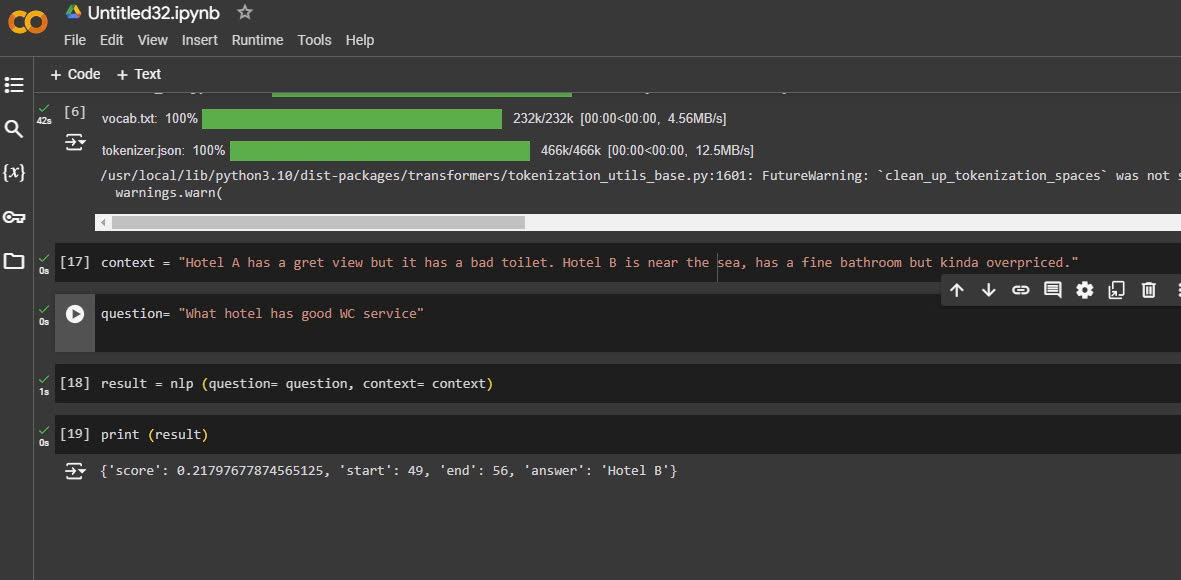
\includegraphics[width=1.0\linewidth]{Figures/IMG_7847.jpeg}
        \caption{Khởi chạy ứng dụng}
        \label{fig:iot}

    \end{figure}
    
    
\end{itemize}


\section*{Kết luận chương}
Trong phần Kết chương, sinh viên đưa ra một số kết luận quan trọng của chương. Những vấn đề mở ra trong Tổng quan cần được tóm tắt lại nội dung và cách giải quyết/thực hiện như thế nào. Sinh viên lưu ý không viết Kết chương giống hệt Tổng quan. Sau khi đọc phần Kết chương, người đọc sẽ nắm được sơ bộ nội dung và giải pháp cho các vấn đề đã trình bày trong chương. Trong Kết chương, Sinh viên nên có thêm câu liên kết tới chương tiếp theo.

Ví dụ về phần Kết chương: Chương này đã phân tích chi tiết sáu nhóm công cụ tích hợp dữ liệu. Nhóm công cụ ABC và DEF thích hợp với những bài toán tích hợp dữ liệu phạm vi nhỏ. Trong khi đó, nhóm công cụ GHK lại chứng tỏ thế mạnh của mình với những bài toán cần độ chính xác cao, v.v. Từ kết quả nghiên cứu và phân tích về sáu nhóm công cụ tích hợp dữ liệu này, lâp trình viên đã thực hiện phát triển phần mềm tự động bóc tách
và tích hợp dữ liệu sử dụng nhóm công cụ GHK. Phần này được trình bày trong chương tiếp theo – Chương 5.

\section{Chủ đề tìm hiểu tuần 7: Thử nghiệm dữ liệu bằng Cosine similarity và Correlation Coefficient}
\subsection{Mục tiêu tuần 7}
Tuần này, lập trình viên đã tiến hành thử nghiệm dữ liệu thu được từ hệ thống đề xuất khách sạn bằng cách tính toán độ tương đồng Cosine và hệ số tương quan Correlation giữa yêu cầu nhập vào của người dùng và các đánh giá của khách hàng về các khách sạn. Mục tiêu là để tìm ra khách sạn phù hợp nhất với nhu cầu của người dùng dựa trên đánh giá của khách hàng.

\subsection{Mục tiêu tuần}
\begin{itemize}
    \item Tiền xử lý dữ liệu đánh giá khách sạn, bao gồm xử lý văn bản từ các đánh giá tích cực và tiêu cực.
    \item Tính toán độ tương đồng Cosine và hệ số tương quan Correlation giữa yêu cầu người dùng và dữ liệu khách sạn.
    \item Xác định khách sạn phù hợp nhất dựa trên kết quả của độ tương đồng và hệ số tương quan.
\end{itemize}

\subsection{Quá trình và phương pháp thực hiện}
\subsubsection{Tiền xử lý dữ liệu}

\begin{figure}[H]
    \centering
    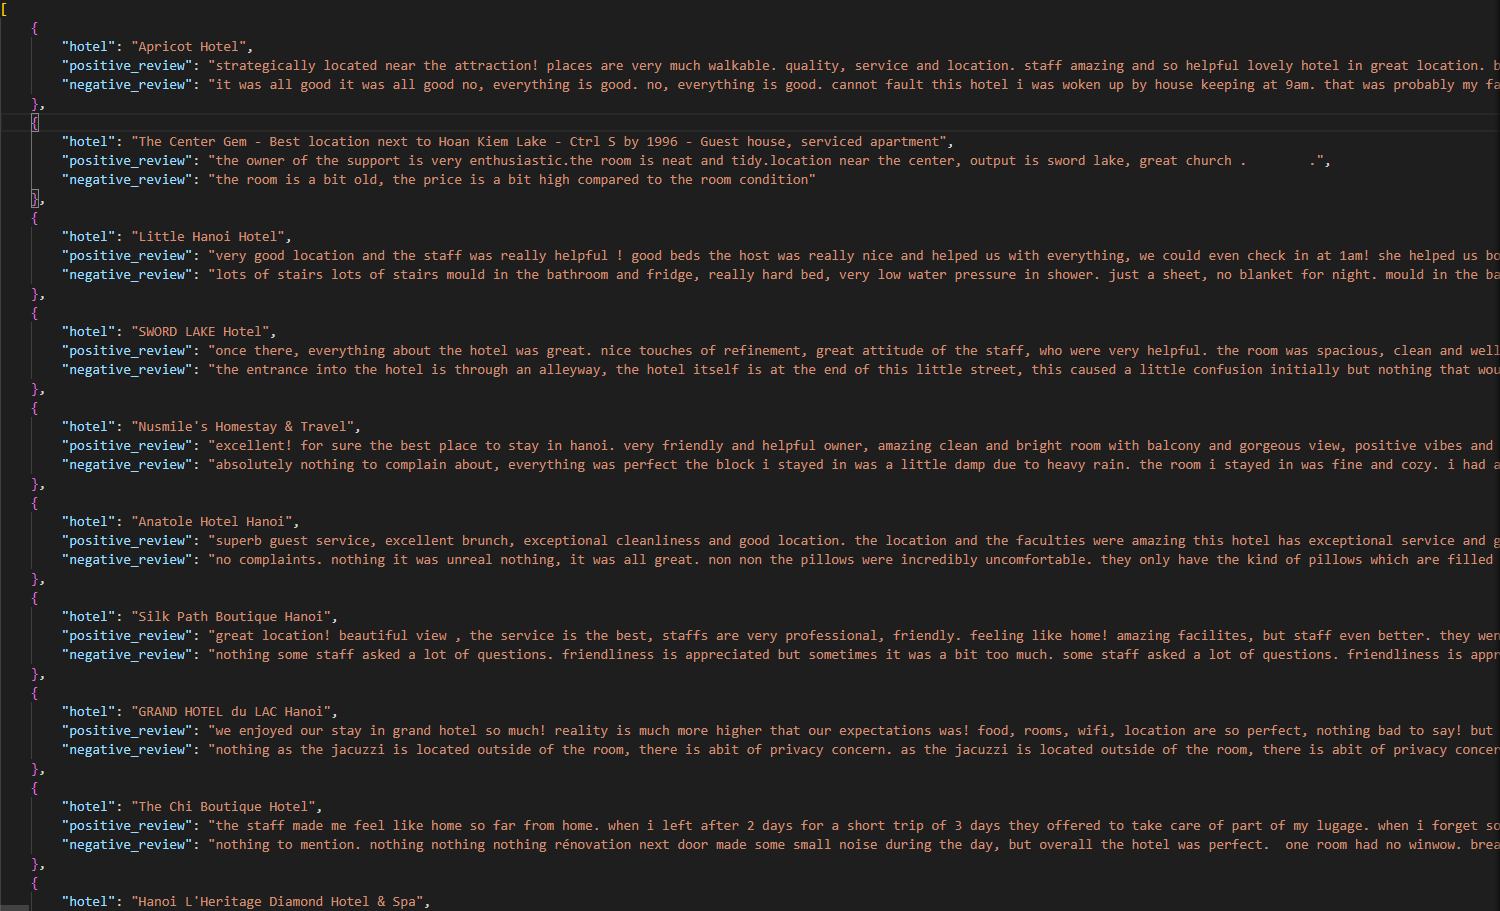
\includegraphics[width=0.9\linewidth]{Figures/preprocess_data.png}
    \caption{Dữ liệu trước khi xử lý}
    \label{fig:enter-label}
\end{figure}

\begin{figure}[H]
    \centering
    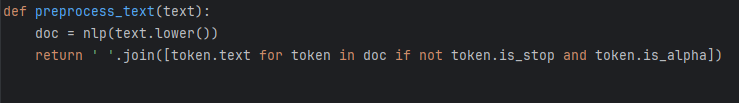
\includegraphics[width=0.9\linewidth]{Figures/pre_process.png}
    \caption{Hàm xử lý}
    \label{fig:enter-label}
\end{figure}
Dữ liệu đánh giá của khách sạn được tải từ file JSON, bao gồm các đánh giá tích cực và tiêu cực từ khách hàng. lập trình viên đã thực hiện tiền xử lý dữ liệu bằng cách chuyển tất cả về chữ thường, loại bỏ các ký tự không phải chữ cái, và loại bỏ các từ dừng (stop words). Điều này giúp giảm bớt nhiễu và cải thiện độ chính xác của mô hình.

\subsubsection{Tạo vector hóa TF-IDF}
\begin{figure}[H]
    \centering
    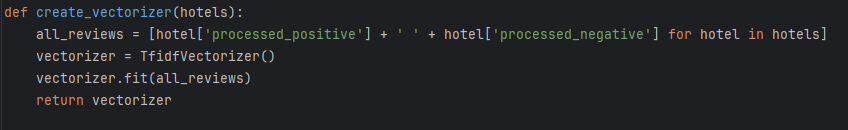
\includegraphics[width=0.9\linewidth]{Figures/TF-IDF.png}
    \caption{vector TF_IDF}
    \label{fig:enter-label}
\end{figure}
Sau khi tiền xử lý, lập trình viên đã tạo các vector TF-IDF cho các đánh giá tích cực và tiêu cực của mỗi khách sạn. Vector TF-IDF giúp biểu diễn dữ liệu văn bản dưới dạng số, từ đó có thể tính toán độ tương đồng giữa yêu cầu của người dùng và các đánh giá khách sạn.

\subsubsection{Tính toán độ tương đồng Cosine và hệ số tương quan}
\begin{itemize}
    \item \textbf{Độ tương đồng Cosine}: lập trình viên đã sử dụng độ tương đồng Cosine để đo lường mức độ giống nhau giữa yêu cầu của người dùng và các đánh giá tích cực, tiêu cực của khách sạn. Độ tương đồng Cosine được tính dựa trên góc giữa hai vector, giúp xác định mức độ liên quan giữa yêu cầu và đánh giá.
    \item \textbf{Hệ số tương quan}: Bên cạnh đó lập trình viên cũng sử dụng hệ số tương quan để đo lường mối quan hệ giữa yêu cầu của người dùng và các đánh giá. Hệ số tương quan giúp xác định mức độ liên hệ tuyến tính giữa hai vector, từ đó tìm ra khách sạn có đánh giá phù hợp nhất với yêu cầu.
\end{itemize}

\subsection{Đánh giá và bài học rút ra}

\begin{figure}[H]
    \centering
    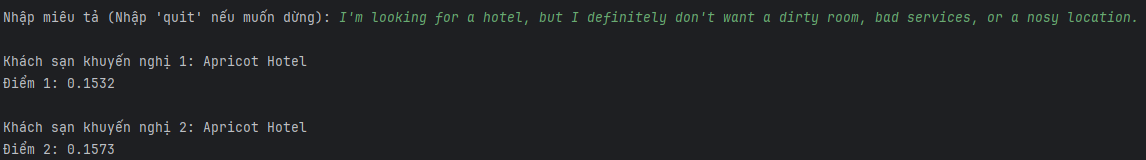
\includegraphics[width=1.0\linewidth]{Figures/Result_cosine_corr.png}
    \caption{Ví dụ đánh giá }
    \label{fig:enter-label}
\end{figure}
Kết quả thử nghiệm cho thấy hai độ đo đã xác định được các khách sạn phù hợp với yêu cầu của người dùng dựa trên đánh giá của khách hàng. Tuy nhiên, điểm khác biệt giữa độ tương đồng Cosine và hệ số tương quan Correlation cần được phân tích kỹ lưỡng hơn để đánh giá hiệu quả của từng phương pháp và chọn ra phương pháp phù hợp nhất trong việc tìm kiếm khách sạn.

\subsection{Kết luận}
Trong tuần này, lập trình viên thử nghiệm với dữ liệu đánh giá thu thập được và sử dụng các phương pháp tính toán độ tương đồng và tương quan để tìm ra khách sạn phù hợp với yêu cầu người dùng. Các kết quả đạt được khá khả quan, tuy nhiên vẫn cần cải thiện thêm để nâng cao hiệu suất của hệ thống.\\
Mô hình trả về kết quả khá tốt nhưng vì kết quả chỉ dựa vào điểm số sự xuất hiện feature trong prompt của user nên kết quả chưa được ổn, vì vậy nhóm đề xuất sử dụng mô hình named entity recognition để mô hình có thể nhận ra được đặc điểm mong muốn và không mong muốn trong prompt.

\begin{figure}[H]
    \centering
    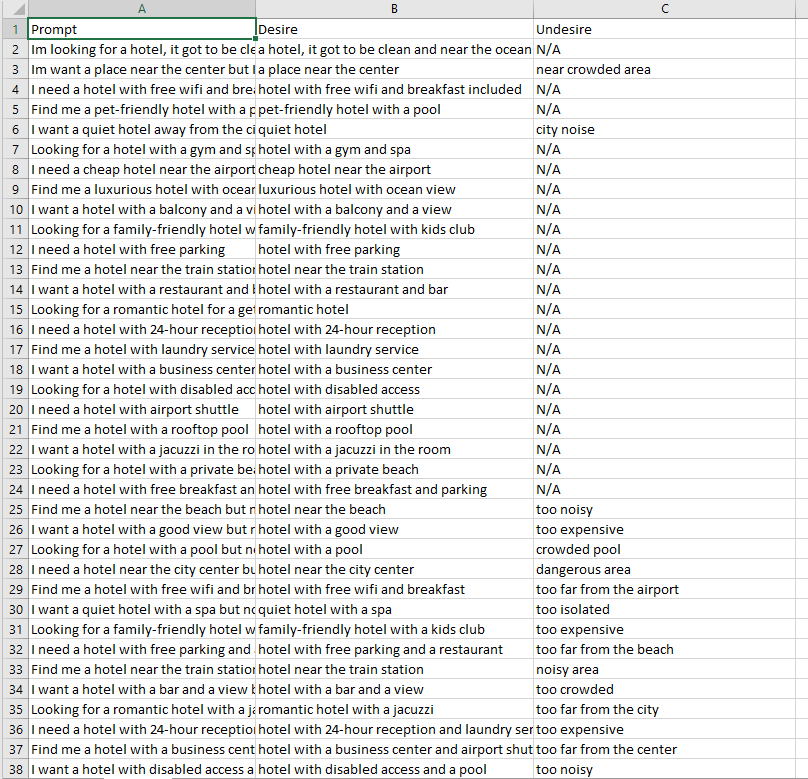
\includegraphics[width=0.9\linewidth]{Figures/prompt_csv.png}
    \caption{File csv nhận được}
    \label{fig:enter-label}
\end{figure}

\begin{figure}[H]
    \centering
    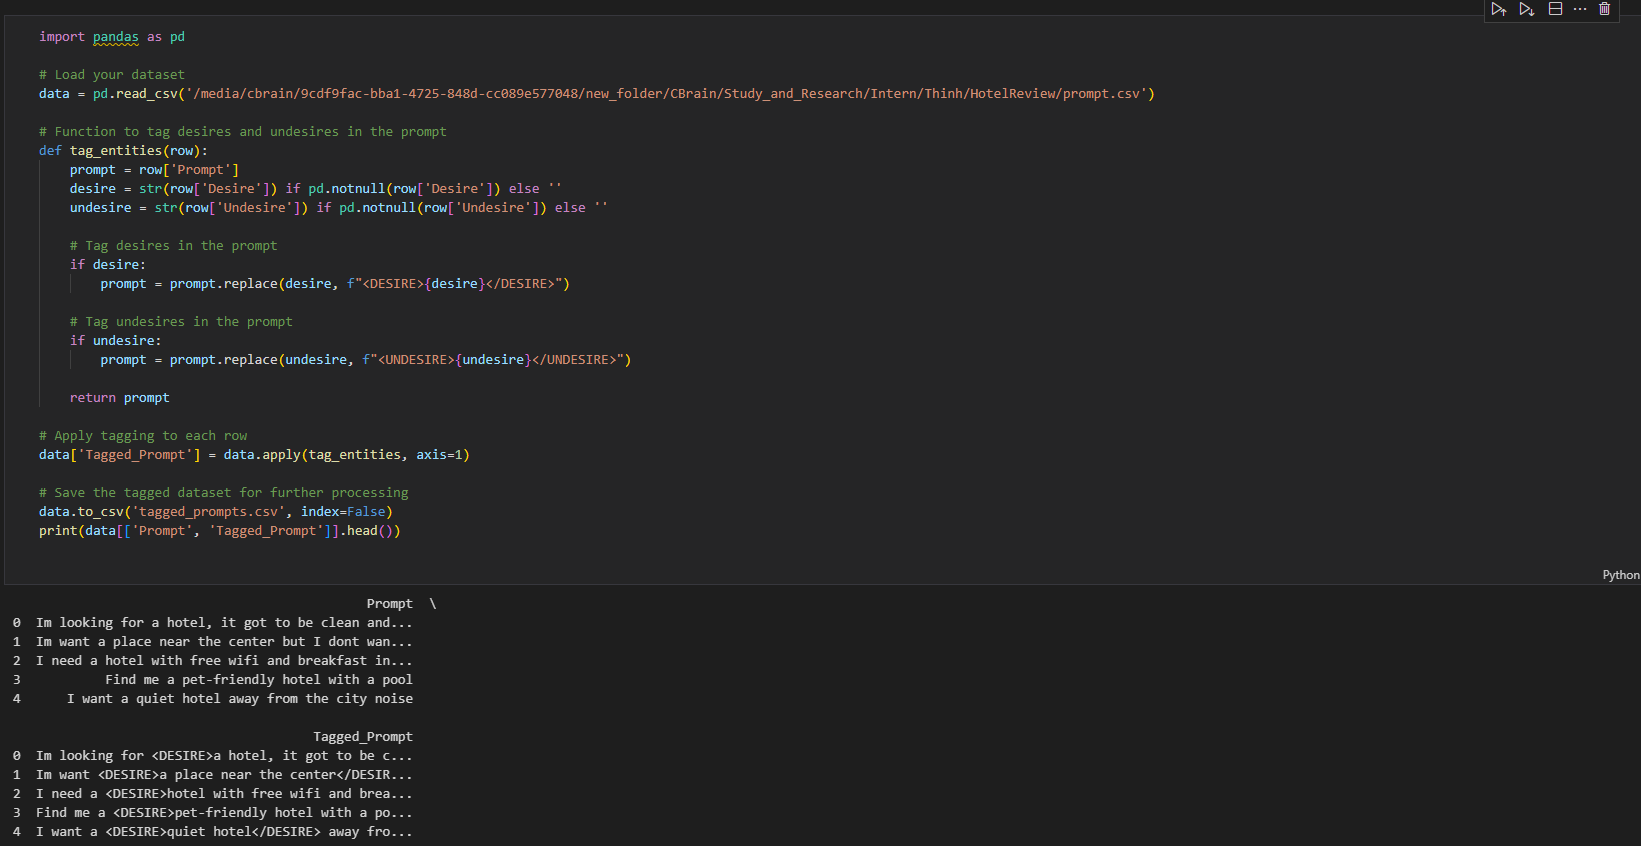
\includegraphics[width=0.8\linewidth]{Figures/code_result_1.png}
    \caption{hàm xử lý}
    \label{fig:enter-label}
\end{figure}

\begin{figure}[H]
    \centering
    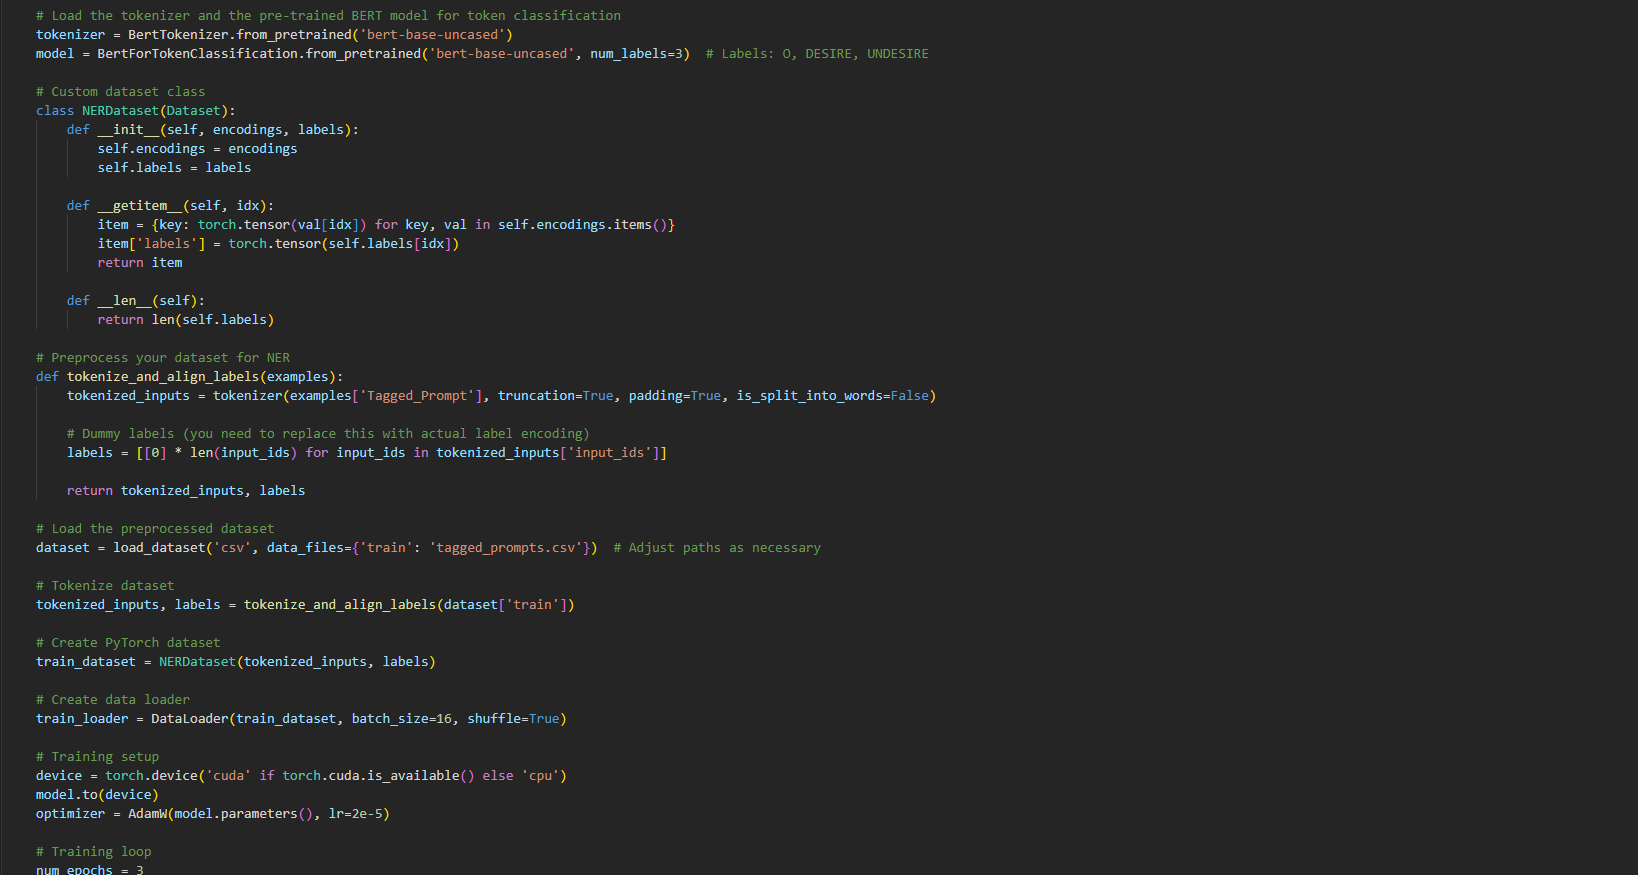
\includegraphics[width=0.8\linewidth]{Figures/code_result_2.png}
    \caption{hàm xử lý}
    \label{fig:enter-label}
\end{figure}

\begin{figure}[H]
    \centering
    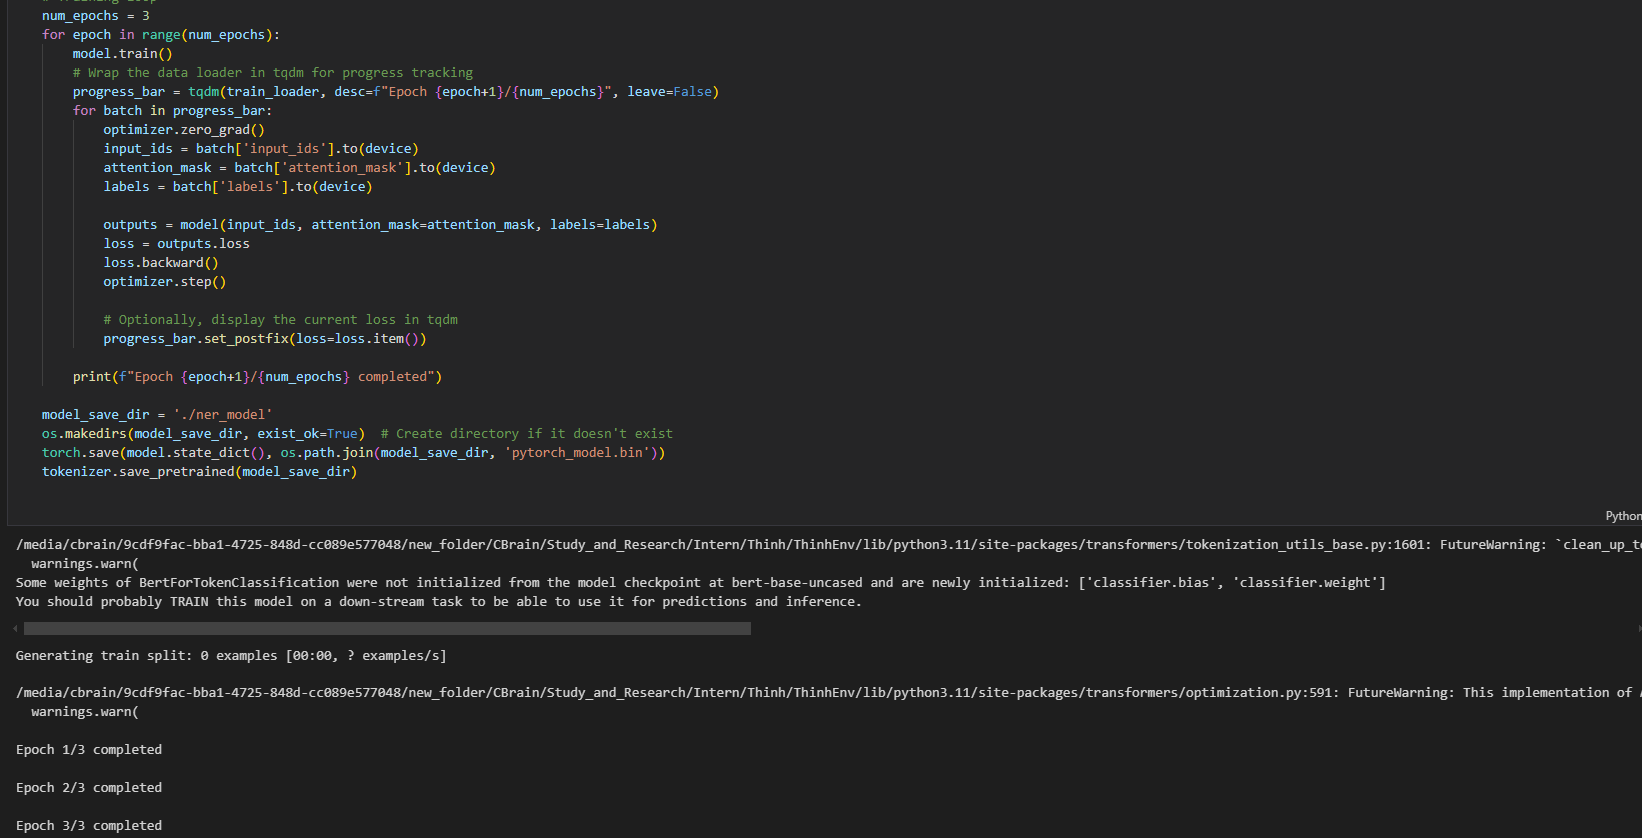
\includegraphics[width=0.8\linewidth]{Figures/code_result_3.png}
    \caption{hàm xử lý}
    \label{fig:enter-label}
\end{figure}

\begin{figure}[H]
    \centering
    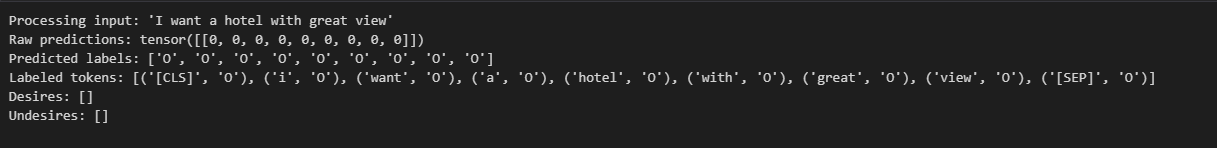
\includegraphics[width=0.8\linewidth]{Figures/result_4_10.png}
    \caption{Kết quả}
    \label{fig:enter-label}
\end{figure}

\section{Chủ đề tìm hiểu tuần 8: Nghiên cứu sử dụng BERTopic để phân cụm bộ dữ liệu positive review và negative review}

\subsection{Mục tiêu tuần 8}
Tuần này, lập trình viên tập trung vào việc sử dụng BERTopic để phân cụm bộ dữ liệu đánh giá tích cực và tiêu cực. BERTopic được chọn nhờ khả năng hiệu suất cao trong việc nắm bắt ngữ cảnh và phân tích chủ đề chính xác hơn so với các phương pháp như LSA hay NMF.

\subsection{Mục tiêu tuần}
\begin{itemize}
    \item Phân cụm dữ liệu đánh giá của khách hàng, bao gồm dữ liệu positive review và negative review.
    \item Tìm hiểu cách BERTopic xử lý ngôn ngữ tự nhiên và trích xuất các chủ đề chính từ dữ liệu.
    \item Gán nhãn cho các chủ đề dựa trên các từ khóa trích xuất từ mỗi cụm.
\end{itemize}

\subsection{Ý tưởng}
Sử dụng mô hình chủ đề (Topic Model) để tách lọc các chủ đề mà khách hàng đề cập đến trong đánh giá của họ. Các chủ đề được đề cập nhiều trong đánh giá sẽ trở thành đặc trưng (feature) cho từng khách sạn. Từ đó, chúng ta có thể phân cụm bộ dữ liệu theo chủ đề của các đánh giá.

\subsection{Giải thích về Mô hình chủ đề (Topic Model)}
Mô hình chủ đề là một phương pháp trong xử lý ngôn ngữ tự nhiên (NLP) dùng để xác định và phân tích các chủ đề trong một tập hợp văn bản. Thông qua việc xác định các chủ đề chính trong tài liệu, chúng ta có thể hiểu rõ hơn về nội dung ý kiến và tâm trạng của người viết. Mô hình chủ đề thường giúp cải thiện khả năng truy xuất thông tin và phân tích cảm xúc trong văn bản.

\textbf{Tại sao sử dụng BERTopic thay vì LSA hay NMF?}
\begin{itemize}
    \item \textbf{Hiệu suất cao hơn:} BERTopic sử dụng mô hình BERT (Bidirectional Encoder Representations from Transformers) để tạo ra các vector nhúng (embeddings) cho các đoạn văn bản. BERT có khả năng nắm bắt ngữ cảnh từ hai phía của văn bản giúp cải thiện độ chính xác trong việc nhận diện chủ đề so với các phương pháp truyền thống như LSA (Latent Semantic Analysis) hay NMF (Non-Negative Matrix Factorization).
    \item \textbf{Khả năng mở rộng và linh hoạt:} BERTopic cho phép phân cụm các đoạn văn bản lớn và có tính năng tự động điều chỉnh số lượng chủ đề, điều này giúp phù hợp với các tập dữ liệu đa dạng.
\end{itemize}

Tóm lại, việc sử dụng BERTopic để phân cụm các đánh giá tích cực và tiêu cực sẽ giúp chúng ta nắm bắt được các chủ đề quan trọng mà khách hàng đề cập đến, từ đó nâng cao khả năng phân tích và đưa ra quyết định cho các dịch vụ của khách sạn.

\begin{enumerate}
    \item \textbf{Xử lý dữ liệu:}
    Đây là một bộ dataset mẫu gồm 70 khách sạn, toàn bộ đánh giá đã được chuyển sang ngôn ngữ Anh và kết nối lại với nhau.

    \begin{figure}[H]
        \centering
        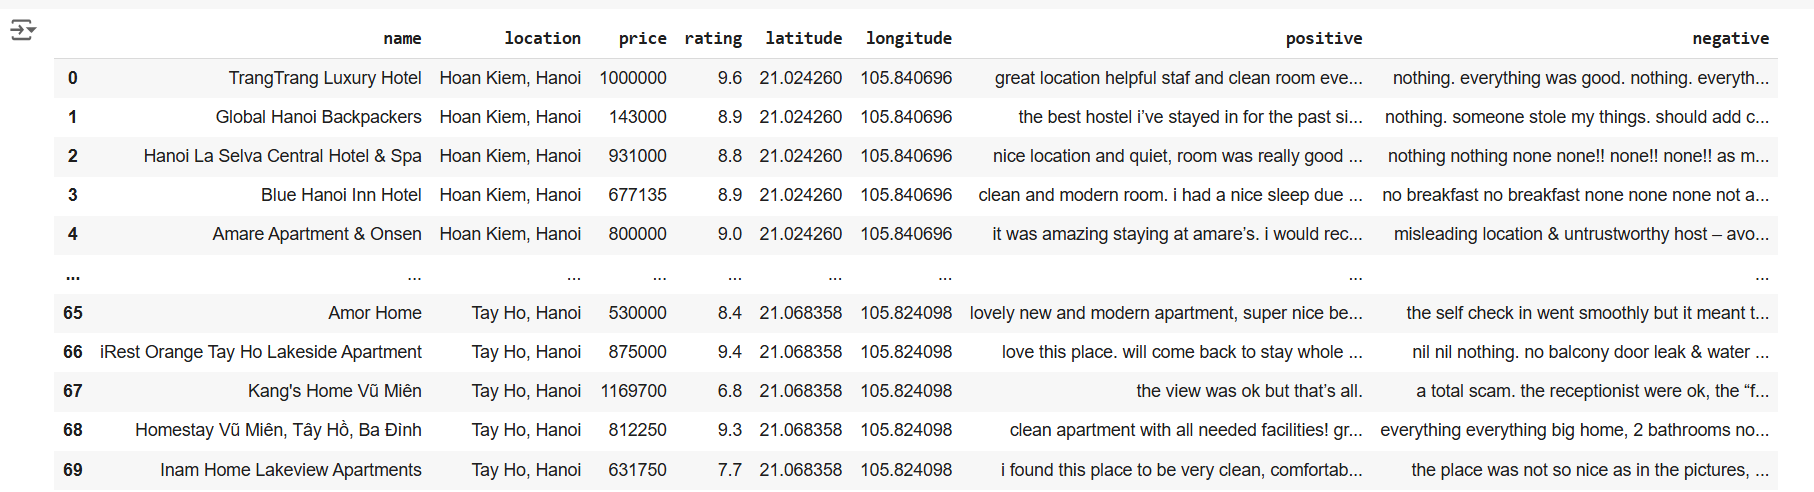
\includegraphics[width=1\linewidth]{Figures/8.1.png}
        \caption{Dữ liệu khách sạn}
        \label{fig:enter-label}
    \end{figure}

    \begin{figure}[H]
        \centering
        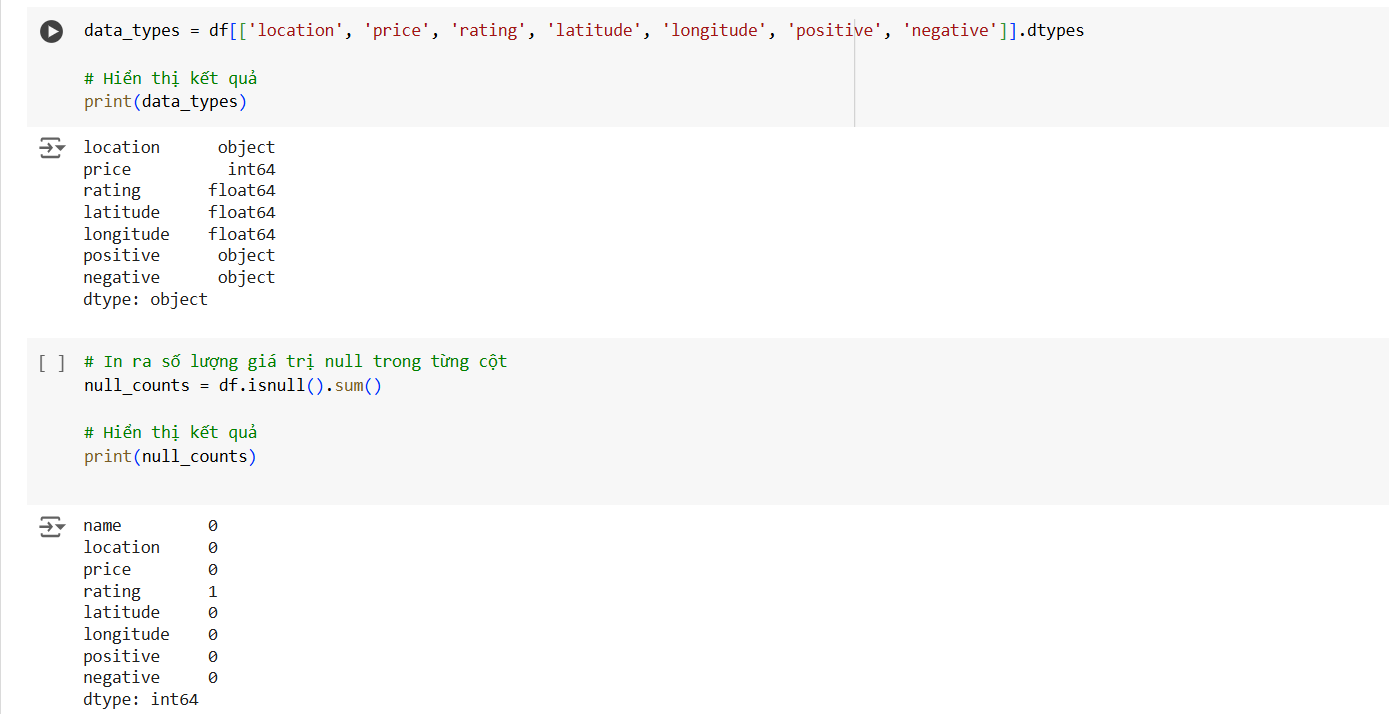
\includegraphics[width=1\linewidth]{Figures/8.2.png}
        \caption{Thông tin khách sạn}
        \label{fig:enter-label}
    \end{figure}

     \begin{figure}[H]
        \centering
        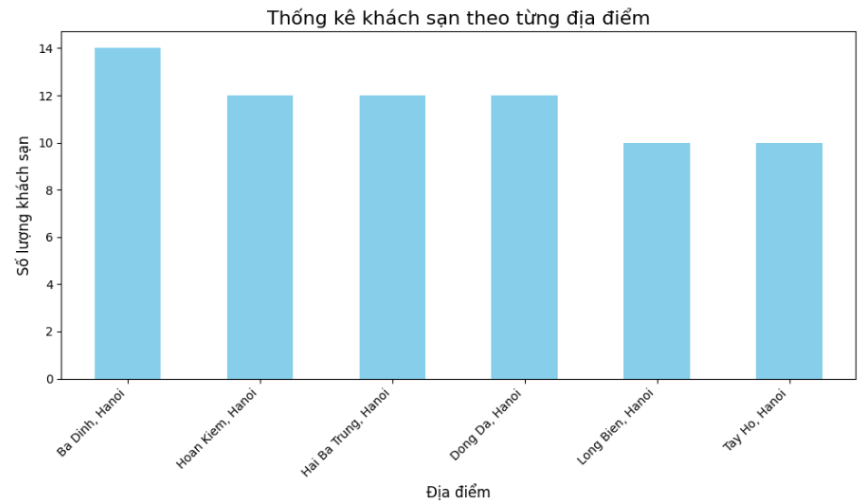
\includegraphics[width=1\linewidth]{Figures/8.3.png}
        \caption{Biểu đồ thống kê khách sạn trong Hà Nội}
        \label{fig:enter-label}
    \end{figure}

     \begin{figure}[H]
        \centering
        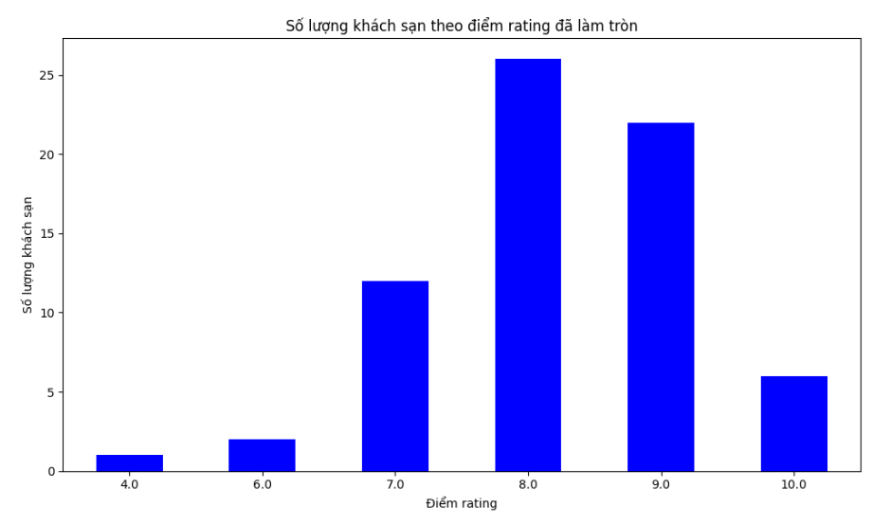
\includegraphics[width=1\linewidth]{Figures/8.4.png}
        \caption{Biểu đồ đánh giá rating}
        \label{fig:enter-label}
    \end{figure}

     \item \textbf{Loại bỏ stopwords và ký tự đặc biệt:}
    Để tối ưu cho quá trình tách lọc chủ đề, lập trình viên loại bỏ toàn bộ stopwords và các ký tự đặc biệt trong dữ liệu.

     \begin{figure}[H]
        \centering
        \includegraphics[width=1\linewidth]{Figures/8.5.png}
        \caption{Hàm tách lọc chủ đề}
        \label{fig:enter-label}
    \end{figure}

    \item \textbf{Bộ dữ liệu negative\_review sau khi làm sạch:}

     \begin{figure}[H]
        \centering
        \includegraphics[width=1\linewidth]{Figures/8.6.png}
        \caption{20 từ phổ biến nhất trong negative}
        \label{fig:enter-label}
    \end{figure}

     \begin{figure}[H]
        \centering
        \includegraphics[width=1\linewidth]{Figures/8.7.png}
        \caption{Biểu đồ các từ phổ biến nhất trong negative}
        \label{fig:enter-label}
    \end{figure}

     \begin{figure}[H]
        \centering
        \includegraphics[width=1\linewidth]{Figures/8.8.png}
        \caption{negative}
        \label{fig:enter-label}
    \end{figure}

    \item \textbf{Bộ dữ liệu positive\_review sau khi làm sạch:}

    \begin{figure}[H]
        \centering
        \includegraphics[width=1\linewidth]{Figures/8.9.png}
        \caption{20 từ phổ biến nhất trong positive}
        \label{fig:enter-label}
    \end{figure}

    \begin{figure}[H]
        \centering
        \includegraphics[width=1\linewidth]{Figures/8.10.png}
        \caption{Biểu đổ từ phổ biến nhất trong positive}
        \label{fig:enter-label}
    \end{figure}

    \begin{figure}[H]
        \centering
        \includegraphics[width=1\linewidth]{Figures/8.11.png}
        \caption{Positive}
        \label{fig:enter-label}
    \end{figure}
    
\end{enumerate}

Tiếp theo, chúng ta bắt đầu tiến vào công đoạn sử dụng mô hình BERTopic

\textbf{Sơ lược về cách BERTopic hoạt động:}

\begin{enumerate}
    \item \textbf{Text Embedding:} BERTopic sử dụng mô hình BERT  (Bidirectional Encoder Representations from Transformers) để biểu diễn văn bản.
    
    \textit{Biểu diễn từ (Word Embedding):} Đây là kỹ thuật giúp chuyển các từ thành các vector số trong không gian đa chiều, trong đó các từ có ngữ nghĩa tương tự nhau sẽ được biểu diễn gần nhau. Điều này giúp máy tính xử lý và hiểu ngôn ngữ tự nhiên hiệu quả hơn.

     \begin{figure}[H]
        \centering
        \includegraphics[width=0.6\linewidth]{Figures/8.12.png}
        \caption{Ví dụ minh họa BERT hoạt động}
        \label{fig:enter-label}
    \end{figure}

    Do BERT là một mô hình tiền huấn luyện nên đã có \textit{một bộ từ điển định sẵn của BERT} với khoảng 30,000 từ (tokens). Đây là một tập hợp các token được tạo ra thông qua tokenization của BERT. Hiểu thêm về Tokenization, đây là quá trình tách một văn bản thành các đơn vị nhỏ hơn là “token”. Đầu tiên, văn bản đầu vào được chuẩn bị bằng cách thêm các ký tự đặc biệt [CLS] ở đầu câu và [SEP] ở cuối để đánh dấu bắt đầu và kết thúc:

     \begin{figure}[H]
        \centering
        \includegraphics[width=0.4\linewidth]{Figures/8.13.png}
        \label{fig:enter-label}
    \end{figure}

    \item \textbf{Phân cụm HDBSCAN}: BERTopic sử dụng thuật toán HDBSCAN để phân cụm các vector nhúng dựa trên mật độ dữ liệu.

    \item \textbf{Trích Xuất Từ Khóa (Keyword Extraction):} Để trích xuất từ khóa cho mỗi chủ đề, BERTopic sử dụng phương pháp TF-IDF.

    \begin{figure}[H]
        \centering
        \includegraphics[width=0.4\linewidth]{Figures/tf.png}
        \label{fig:enter-label}
    \end{figure}

    \begin{figure}[H]
        \centering
        \includegraphics[width=0.4\linewidth]{Figures/idf.png}
        \label{fig:enter-label}
    \end{figure}

    \begin{figure}[H]
        \centering
        \includegraphics[width=0.4\linewidth]{Figures/tfidf.png}
        \label{fig:enter-label}
    \end{figure}

    \item \textbf{Gán Nhãn Chủ Đề (Topic Labeling):} Cuối cùng, mô hình gán nhãn cho các chủ đề dựa trên các từ khóa đã trích xuất. Từ khóa có giá trị TF-IDF cao nhất trong mỗi chủ đề sẽ được dùng để đặt tên cho chủ đề đó.

    Kết quả thu được

    \begin{figure}[H]
        \centering
        \includegraphics[width=1\linewidth]{Figures/8.14.png}
        \caption{Kết quả gán nhãn chủ đề}
        \label{fig:enter-label}
    \end{figure}

    Dũ liệu được cluster về 3 topic, topic -1 là dữ liệu outlier

     \begin{figure}[H]
        \centering
        \includegraphics[width=1\linewidth]{Figures/8.15.png}
        \label{fig:enter-label}
    \end{figure}

     \begin{figure}[H]
        \centering
        \includegraphics[width=1\linewidth]{Figures/8.16.png}
        \caption{Topic Word Scores}
        \label{fig:enter-label}
    \end{figure}

     \begin{figure}[H]
        \centering
        \includegraphics[width=1\linewidth]{Figures/8.18.png}
        \caption{Hiearchical Clustering}
        \label{fig:enter-label}
    \end{figure}

    Do số lượng topic đang khá ít nên sẽ không group các cluster lại

     \begin{figure}[H]
        \centering
        \includegraphics[width=1\linewidth]{Figures/8.19.png}
        \caption{Ví dụ minh họa}
        \label{fig:enter-label}
    \end{figure}

     \begin{figure}[H]
        \centering
        \includegraphics[width=1\linewidth]{Figures/8.20.png}
        \label{fig:enter-label}
    \end{figure}

    Những dữ liệu không được mô hình cluster và gắn -1 thì chúng ta có thể dùng KNN để gắn nhãn tạm thời:

    \begin{figure}[H]
        \centering
        \includegraphics[width=1\linewidth]{Figures/8.21.png}
        \caption{Hàm thực thi}
        \label{fig:enter-label}
    \end{figure}

    \begin{figure}[H]
        \centering
        \includegraphics[width=1\linewidth]{Figures/8.22.png}
        \caption{Kết quả nhân được}
        \label{fig:enter-label}
    \end{figure}
    
    
\end{enumerate}

\subsection{Kết quả thu được}
Dữ liệu được phân cụm thành 3 topic. Các dữ liệu không được phân cụm được gắn nhãn "-1". lập trình viên có thể sử dụng KNN để gán nhãn tạm thời cho các dữ liệu này.





\section{Chủ đề tìm hiểu tuần 9: Nghiên cứu sử dụng BERT dựa vào review của khách hàng để chấm điểm cho các khách sạn thiếu rating}

\setcounter{figure}{0} % Đặt lại bộ đếm hình ảnh về 0
\renewcommand{\thefigure}{4.\arabic{figure}}

\subsection{Mục tiêu tuần 9}
  Hiểu rõ cách thức hoạt động của mô hình BERT (Bidirectional Encoder Representations from Transformers) và cách mà nó có thể được áp dụng trong các bài toán , áp dụng mô hình BERT để phát triển một hệ thống có khả năng dự đoán rating cho các khách sạn dựa trên review của khách hàng, đặc biệt là cho những khách sạn không có rating sẵn.


    \subsection{Bài toán}
Một số khách sạn không có điểm số rating cụ thể trên \textbf{Booking.com}. Để giải quyết vấn đề này, lập trình viên xây dựng một hệ thống dự đoán điểm số dựa trên review của khách hàng. Hệ thống này sử dụng mô hình BERT để phân tích nội dung review và gán điểm rating phù hợp cho các khách sạn chưa được đánh giá.

\subsection{Phương pháp tiếp cận}
Để giải quyết bài toán trên, lập trình viên đã áp dụng các bước sau:

\subsubsection{Chuẩn bị dữ liệu}
Dữ liệu bao gồm hai cột: \texttt{Positive\_Review} và \texttt{Negative\_Review}, được kết hợp để tạo thành chuỗi văn bản đầu vào duy nhất:
\begin{figure}[H]
        \centering
        \includegraphics[width=1\linewidth]{Figures/9.1.png}
        \caption{Dự liệu được chuẩn bị}
        \label{fig:enter-label}
    \end{figure}
\begin{verbatim}
data['combined_review'] = data['Positive_Review'] + " " + data['Negative_Review']
\end{verbatim}

\subsubsection{Xây dựng mô hình}
- **Tokenizer**: Sử dụng \texttt{BertTokenizer} để chuyển đổi review thành các vector token.
- **Model**: Áp dụng \texttt{AutoModelForSequenceClassification} với nhãn đầu ra là 1 cho bài toán hồi quy.


\begin{figure}[H]
        \centering
        \includegraphics[width=1\linewidth]{Figures/9.2.png}
        \label{fig:enter-label}
    \end{figure}

\subsubsection{Huấn luyện mô hình}
Áp dụng hàm mất mát MSE và tối ưu hóa với AdamW. Mô hình được huấn luyện trong 3 epoch:

\begin{figure}[H]
        \centering
        \includegraphics[width=1\linewidth]{Figures/9.3.png}
        \label{fig:enter-label}
    \end{figure}

\subsubsection{Dự đoán rating}
Mô hình đã được huấn luyện sẽ được sử dụng để dự đoán rating cho các khách sạn thiếu dữ liệu:

\begin{figure}[H]
        \centering
        \includegraphics[width=1\linewidth]{Figures/9.4.png}
        \label{fig:enter-label}
    \end{figure}

\subsubsection{Lưu kết quả}
Kết quả dự đoán được ghi vào file CSV:

\begin{verbatim}
data.loc[data['Rating'].isna(), 'Rating'] = predicted_ratings
data.to_csv('output2.csv', index=False)
\end{verbatim}

\section{Kết quả và đánh giá}
- Mô hình BERT đã được huấn luyện thành công và có thể dự đoán điểm số rating dựa trên nội dung review.  
- Việc này giúp cải thiện hệ thống đề xuất khách sạn, đảm bảo cung cấp thông tin đầy đủ hơn cho người dùng.
\begin{figure}[H]
        \centering
        \includegraphics[width=1\linewidth]{Figures/9.5.png}
        \caption{Kết quả mô hình BERT được huấn luyện}
        \label{fig:enter-label}
    \end{figure}

\section{Chủ đề tìm hiểu tuần 10: Phân cụm dữ liệu review khách sạn với Orange Data Mining}

\subsection{Mục tiêu tuần 10}
Mục tiêu chính của tuần này là phân cụm dữ liệu review khách sạn (positive review và negative review) để tìm hiểu xu hướng đặt phòng của khách hàng. lập trình viên đã sử dụng các công cụ Orange Data Mining để thực hiện quá trình phân cụm này, áp dụng thuật toán K-Means để thực hiện phân cụm với số lượng k = 10 sau khi giảm chiều dữ liệu bằng PCA.

\subsection{Bài toán}
Phân tích và nhóm các khách sạn dựa trên nội dung review của khách hàng trên các nền tảng đặt phòng trực tuyến \textbf{Booking.com}. Điều này giúp xác định các nhóm khách sạn có cùng xu hướng về mức độ hài lòng, không hài lòng và các đặc điểm liên quan giữa các khách sạn này.

\subsection{Phương pháp tiếp cận}
lập trình viên đã áp dụng các bước sau trong Orange Data Mining:

\subsubsection{Chuẩn bị dữ liệu}
\begin{itemize}
    \item Đầu tiên dữ liệu được tải lên Orange Data Mining bằng widget \textbf{\textit{File}} và được hiển thị với widget \textbf{\textit{Data Table}} như hình bên dưới đây.

    \begin{figure}[H]
        \centering
        \includegraphics[width=0.5\linewidth]{Figures/10.1.png}
        \label{fig:enter-label}
    \end{figure}

    \item Dữ liệu được thu thập từ các review của khách sạn trên trang web \textbf{Booking.com}, với ba trường chính là \textbf{\textit{Positive Review}}, \textbf{\textit{Negative Review}} và \textbf{\textit{Rating}} tương ứng với điểm số của khách sạn. 

    \begin{figure}[H]
        \centering
        \includegraphics[width=1.0\linewidth]{Figures/10.2.png}
        \caption{Dự liệu được thu thập}
        \label{fig:enter-label}
    \end{figure}

    \item Sau đó dữ liệu sẽ được đưa vào widget \textbf{\textit{Corpus}} để chọn ra các feature và ngôn ngữ chính cho bộ dữ liệu.

    \begin{figure}[H]
        \centering
        \includegraphics[width=0.5\linewidth]{Figures/10.3.png}
        \label{fig:enter-label}
    \end{figure}

    \begin{figure}[H]
        \centering
        \includegraphics[width=0.5\linewidth]{Figures/10.4.png}
        \label{fig:enter-label}
    \end{figure}
\end{itemize}
\subsubsection{Xử lý dữ liệu}
Sau khi dữ liệu được tải lên thành công, lập trình viên tiến hành với bước tiền xử lý dữ liệu. Dữ liệu được tiền xử lý để chuyển tất cả thành chữ thường, loại bỏ các từ dừng (stopwords), tách dữ liệu thành các câu và đưa các từ trong câu về dạng ban đầu (lemmatizer). Để thực hiện công việc này, lập trình viên sử dụng \textbf{\textit{Preprocess Text}} của Orange.

\begin{figure}[H]
    \centering
    \includegraphics[width=0.5\linewidth]{Figures/10.5.png}
    \label{fig:enter-label}
\end{figure}

\begin{figure}[H]
    \centering
    \includegraphics[width=1\linewidth]{Figures/10.6.png}
    \caption{Quá trình Xử lý dữ liệu}
\end{figure}

\subsubsection{Document Embedding}
Sau khi tiền xử lý dữ liệu, lập trình viên sử dụng công widget \textbf{\textit{Document Embedding}} để chuyển đổi các review thành vector số bằng fastText để làm dữ liệu đầu vào cho các bước phân tích tiếp theo.

\begin{figure}[H]
    \centering
    \includegraphics[width=0.5\linewidth]{Figures/10.7.png}
\end{figure}

\begin{figure}[H]
    \centering
    \includegraphics[width=0.5\linewidth]{Figures/10.8.png}
\end{figure}


\subsubsection{Giảm chiều dữ liệu với PCA}
Dữ liệu sau khi được embedding có kích thước lớn, vì thế lập trình viên áp dụng phương pháp Principal Component Analysis (PCA) để giảm chiều dữ liệu, lấy ra nhưng đặc trưng chính trong dữ liệu, giúp tối ưu quá trình phân cụm.

\begin{figure}[H]
    \centering
    \includegraphics[width=0.6\linewidth]{Figures/10.9.png}
\end{figure}

\begin{figure}[H]
    \centering
    \includegraphics[width=0.9\linewidth]{Figures/10.10.png}
    \caption{}
\end{figure}

\subsubsection{Phân cụm với K-Means}
Sau khi embedding, lập trình viên sử dụng thuật toán K-Means cho việc phân cụm dữ liệu review. lập trình viên áp dụng thuậ toán K-Means với số cụm k được đặt là 10, số lượng cụm vừa đủ để có thể phân tích các đặc điểm của các khách sạn với nhau.

\begin{figure}[H]
    \centering
    \includegraphics[width=0.5\linewidth]{Figures/10.11.png}
\end{figure}

\begin{figure}[H]
    \centering
    \includegraphics[width=0.6\linewidth]{Figures/10.12.png}
    \caption{Phân cụm dữ liệu}
\end{figure}

\subsection{Kết quả và đánh giá}
Kết quả từ quá trình phân cụm được trực quan hóa bằng biểu đồ Scatter Plot:

\begin{figure}[H]
    \centering
    \includegraphics[width=1\linewidth]{Figures/10.13.png}
    \caption{Kết quả nhận được khi phân cụm}
\end{figure}

Từ hình ảnh kết quả phân cụm, lập trình viên rút ra một số nhận xét như sau:
\begin{itemize}
    \item \textbf{Cụm 1 (C1):} Có các khách sạn tiêu biểu đại diện cho cụm như Hanoi Hola House và Le Grand Hanoi Hotel. Các khách sạn này có xu hướng nhận các đánh giá tích cực từ khách hàng với điểm số trung bình cao.

    \item \textbf{Cụm 2 (C2):} Có các khách sạn tiêu biểu đại diện cho cụm như Hoang Long Hotel và Hortensia Full. Khách sạn trong cụm này có thể có mức độ hài lòng trung bình, với sự đa dạng trong các đánh giá.

    \item \textbf{Cụm 3 - Cụm 6:} Một số khách sạn tiểu biểu đại diện cho cụm như Vintage House và Bamboo Home ở cụm 5 nhận được các đánh giá có nhiều yếu tố tích cực, tuy nhiên, cũng có một số điểm hạn chế, đặc biệt là trong đánh giá negative review, thể hiện qua việc một số khách sạn có tên trong các cụm thấp hơn.

    \item \textbf{Cụm 7 - Cụm 8:} Tập trung vào các khách sạn có vị trí tốt và không gian thoải mái nhưng cần cải thiện về dịch vụ để đạt được sự ổn định trong đánh giá của khách hàng.

    \item \textbf{Cụm 9 - Cụm 10:} Đại diện cho những khách sạn/homestay có trải nghiệm độc đáo về mặt thiết kế và vị trí, nhưng chất lượng dịch vụ không đồng nhất là một điểm cần chú ý.
\end{itemize}

Để rõ ràng hơn giữa các cụm, lập trình viên có 1 số nhận xét chi tiết như sau:

\begin{itemize}
    \item \textbf{Cụm 1 - Cụm 2:} Nhận được đánh giá tích cực về vị trí và dịch vụ. Các khách sạn trong cụm 1, như Hanoi Hola House và Le Grand Hanoi Hotel, có xu hướng đạt điểm số cao nhờ vào sự ổn định trong dịch vụ và vị trí thuận tiện. Tuy nhiên, cụm 2, bao gồm Hoang Long Hotel và Hortensia Full, có nhiều đánh giá trái chiều hơn, phản ánh sự không đồng đều về chất lượng dịch vụ và tiện nghi. Điều này khiến các khách sạn trong cụm 2 cần tập trung cải thiện để nâng cao sự hài lòng của khách hàng.

    \item \textbf{Cụm 3 - Cụm 6:} Các khách sạn trong các cụm này, như Vintage House và Bamboo Home (thuộc cụm 5), đều có nhiều yếu tố tích cực liên quan đến không gian sống, tiện nghi và vị trí. Tuy nhiên, những điểm yếu về chất lượng dịch vụ và tiện ích chưa hoàn thiện là lý do khiến các khách sạn này không đạt được điểm đánh giá cao hơn. Để nâng cao trải nghiệm khách hàng, các khách sạn cần tập trung cải thiện dịch vụ khách hàng và đảm bảo các tiện ích đáp ứng kỳ vọng của du khách.

    \item \textbf{Cụm 7 - Cụm 8:} Các khách sạn trong cụm 7 và 8, như Vintage House in Central of Old Quarter 2 Bedrooms with Healing Vibe (C7) và Migo Housing Dak Kim Street - Local Flat (C8), có vị trí tốt và không gian sống thoải mái. Tuy nhiên, các khách sạn này gặp vấn đề với chất lượng dịch vụ không ổn định, dẫn đến trải nghiệm không đồng đều. Khách hàng đánh giá cao sự tiện lợi và không gian, nhưng dịch vụ chưa nhất quán khiến điểm số không đạt mức cao nhất. Cải thiện chất lượng dịch vụ sẽ là yếu tố quan trọng để các khách sạn trong nhóm này tăng điểm đánh giá.

    \item \textbf{Cụm 9 - Cụm 10:}Các khách sạn trong cụm 9 và 10, như POMELO - Sun's Homestay - Lake View (C9) và TWINS HOME (C10), nổi bật về thiết kế độc đáo và vị trí đẹp, thu hút du khách với những trải nghiệm thú vị và không gian sáng tạo. Tuy nhiên, sự thiếu nhất quán trong chất lượng dịch vụ đã ảnh hưởng đến sự hài lòng tổng thể của khách hàng. Để cải thiện điểm số và tạo ra sự hài lòng đồng đều, các khách sạn trong nhóm này cần chú trọng đến việc chuẩn hóa quy trình phục vụ và đảm bảo chất lượng dịch vụ nhất quán cho mọi khách hàng.
\end{itemize}

\subsection{Kết luận}
Sử dụng Orange Data Mining để phân cụm dữ liệu review khách sạn đã giúp phân loại các nhóm khách sạn dựa trên mức độ hài lòng của khách hàng. Các cụm được phân chia cho thấy rõ những nhóm khách sạn có đánh giá cao và ổn định về vị trí và dịch vụ, cũng như các nhóm cần cải thiện về tiện ích và dịch vụ để nâng cao trải nghiệm khách hàng. Nhóm các khách sạn có thiết kế độc đáo nhưng dịch vụ không nhất quán cũng được xác định rõ ràng. Kết quả này giúp doanh nghiệp hiểu sâu hơn về xu hướng đánh giá của khách hàng và đưa ra các chiến lược cải thiện chất lượng dịch vụ hiệu quả.

\section{Chủ đề tìm hiểu tuần 11: Thực hành truy vấn trên bộ dữ liệu thô và bộ dữ liệu đã được tiền xử lý}

\setcounter{figure}{0} % Đặt lại bộ đếm hình ảnh về 0
\renewcommand{\thefigure}{5.\arabic{figure}}

\subsection{Mục tiêu tuần 11} 
Mục tiêu chính của tuần này là thực hiện các truy vấn mẫu trên hai bộ dữ liệu: dữ liệu thô (Crawl\_data) và dữ liệu đã được tiền xử lý (Processing\_data) bằng cơ sở dữ liệu không quan hệ (NoSql) MongoDB, qua đó đánh giá hiệu quả của việc tiền xử lý dữ liệu đối với tốc độ và độ chính xác của truy vấn. Các câu truy vấn mẫu tập trung vào nhu cầu thực tế của người dùng trong việc tìm kiếm các khách sạn phù hợp dựa trên tiêu chí giá cả, đánh giá và các yếu tố đặc trưng khác.

\subsection{Bài toán} 
Thực hiện truy vấn dữ liệu khách sạn ở Hà Nội từ hai bộ dữ liệu thô và đã tiền xử lý, nhằm đánh giá hiệu quả của các truy vấn khi áp dụng các tiêu chí về giá cả, vị trí, và đánh giá của khách hàng. Bài toán hướng đến việc kiểm tra sự cải thiện về độ chính xác và tốc độ truy vấn sau khi dữ liệu được làm sạch và chuẩn hóa, từ đó hỗ trợ phân tích sâu hơn về các yếu tố tạo nên trải nghiệm tốt và các điểm cần cải thiện của khách sạn.

\subsection{Phương pháp tiếp cận}
Đầu tiên đó là việc khởi tạo dữ liệu trong MongoDB được thực hiện tuần tự theo các bước như sau:

\subsubsection{Tạo cơ sở dữ liệu}
Việc cần làm đầu tiên đó là chúng ta phải tạo cơ sở dữ liệu để thực hiện truy vấn trên data như sau:

\begin{figure}[H]
    \centering
    \includegraphics[width=0.5\linewidth]{Figures/11.1.png}
    \caption{Tạo cơ sở dữ liệu}
\end{figure}

Sau khi tạo cơ sở dữ liệu cùng với cột Collection tương ứng, ta bắt đầu import data cho các bước truy vấn:

\begin{figure}[H]
    \centering
    \includegraphics[width=0.9\linewidth]{Figures/11.2.png}
    \caption{Import dữ liệu}
\end{figure}

Tạo Collection tương ứng với bộ dữu liệu còn lại, ta có được kết quả như ảnh sau:

\begin{figure}[H]
    \centering
    \includegraphics[width=1.0\linewidth]{Figures/11.3.png}
    \caption{Cơ sở dữ liệu}
\end{figure}

\subsubsection{Câu truy vấn}
lập trình viên đã tạo ra 10 câu truy vấn dựa trên các tiêu chí thường gặp của khách hàng khi chọn khách sạn, như vị trí, giá cả, và tiện nghi. Các truy vấn này giúp kiểm tra khả năng đáp ứng nhu cầu tìm kiếm của bộ dữ liệu thô và dữ liệu đã tiền xử lý, qua đó có thể đánh giá được chất lượng của dữ liệu cũng như tốc độ truy vấn trước và sau khi xử lý dữ liệu.

Các câu truy vấn được dùng cho hai bộ dữ liệu lần lượt như sau:

\begin{enumerate} 
    \item Tôi muốn tìm một khách sạn ở Hoàn Kiếm, Hà Nội với giá dưới 0.03, xếp hạng từ 8 trở lên và được đánh giá tích cực về vị trí và sự thân thiện của nhân viên.

    \begin{verbatim}
    db.translated_hotel_reviews.find({
      location: /Hoan Kiem, Hanoi/i,
      Price: { $lt: 0.03 },
      rating: { $gte: 8 },
      positive_review: /location|staff|friendly/i
    })
    \end{verbatim}

    \item Có khách sạn nào ở Hà Nội với giá từ 0.02 đến 0.05, được khen ngợi về tiện nghi phòng và không gian yên tĩnh không?
    
    \begin{verbatim}
    db.translated_hotel_reviews.find({
      location: /Hanoi/i,
      Price: { $gte: 0.02, $lte: 0.05 },
      positive_review: /amenities|quiet/i
    })
    \end{verbatim}

    \item Khách sạn nào ở khu vực trung tâm Hà Nội có xếp hạng từ 8.5 trở lên, giá không vượt quá 0.04 và nhận được nhiều đánh giá tích cực về cảnh quan và không gian rộng rãi?

    \begin{verbatim}
    db.translated_hotel_reviews.find({
      location: /center|Hanoi/i,
      rating: { $gte: 8.5 },
      Price: { $lte: 0.04 },
      positive_review: /view|space/i
    })
    \end{verbatim}

    \item Tôi đang tìm khách sạn ở Hoàn Kiếm, Hà Nội, với giá dưới 0.04, xếp hạng trên 8, và được đánh giá cao về dịch vụ khách hàng và chất lượng phòng.

    \begin{verbatim}
    db.translated_hotel_reviews.find({
      location: /Hoan Kiem, Hanoi/i,
      Price: { $lt: 0.04 },
      rating: { $gt: 8 },
      positive_review: /service|room/i
    })
    \end{verbatim}

    \item Có khách sạn nào ở Hà Nội, với giá không quá 0.03 và được khen ngợi về sự sạch sẽ, thái độ thân thiện của nhân viên và không gian phòng rộng rãi không?

    \begin{verbatim}
    db.translated_hotel_reviews.find({
      location: /Hanoi/i,
      Price: { $lte: 0.03 },
      positive_review: /clean|friendly|space/i
    })
    \end{verbatim}

    \item Khách sạn nào ở Hà Nội có giá từ 0.03 đến 0.05, xếp hạng trung bình từ 8.5 trở lên và nhận được đánh giá tốt về tiện nghi, an toàn và sự yên tĩnh?

    \begin{verbatim}
    db.translated_hotel_reviews.aggregate([
      { $match: { location: /Hanoi/i, Price: { $gte: 0.03, $lte: 0.05 }, rating: { $gte: 8.5 } } },
      { $group: { _id: "$Hotel_name", avgRating: { $avg: "$rating" }, avgPrice: { $avg: "$Price" } } },
      { $match: { positive_review: /amenities|safe|quiet/i } }
    ])
    \end{verbatim}

    \item Tôi muốn biết khách sạn nào ở Hoàn Kiếm, Hà Nội có xếp hạng từ 8 trở lên, giá dưới 0.05, có đánh giá tốt về vị trí nhưng phàn nàn về tiếng ồn và không gian nhỏ.

    \begin{verbatim}
    db.translated_hotel_reviews.find({
      location: /Hoan Kiem, Hanoi/i,
      rating: { $gte: 8 },
      Price: { $lt: 0.05 },
      positive_review: /location/i,
      negative_review: /noisy|small/i
    })
    \end{verbatim}

    \item Khách sạn nào ở Hà Nội, giá từ 0.02 đến 0.04, xếp hạng trên 8.5, có đánh giá tốt về tiện nghi nhưng lại có nhiều phàn nàn về tốc độ internet hoặc wifi?

    \begin{verbatim}
    db.translated_hotel_reviews.find({
      location: /Hanoi/i,
      Price: { $gte: 0.02, $lte: 0.04 },
      rating: { $gte: 8.5 },
      positive_review: /amenities/i,
      negative_review: /wifi|internet/i
    })
    \end{verbatim}

    \item Có khách sạn nào ở Hà Nội với giá dưới 0.05, xếp hạng từ 8 trở lên, nhận được phản hồi tích cực về vị trí nhưng phàn nàn về chất lượng phòng cũ hoặc nội thất lỗi thời không?

    \begin{verbatim}
    db.translated_hotel_reviews.find({
      location: /Hanoi/i,
      Price: { $lt: 0.05 },
      rating: { $gte: 8 },
      positive_review: /location/i,
      negative_review: /old|outdated|furniture/i
    })
    \end{verbatim}

    \item Tôi muốn tìm các khách sạn ở Hà Nội có xếp hạng từ 8 trở lên, giá từ 0.03 đến 0.06, với đánh giá tốt về cảnh quan nhưng phàn nàn về chất lượng đồ ăn và bữa sáng.

    \begin{verbatim}
    db.translated_hotel_reviews.find({
      location: /Hanoi/i,
      Price: { $gte: 0.03, $lte: 0.06 },
      rating: { $gte: 8 },
      positive_review: /view/i,
      negative_review: /food|breakfast|dining/i
    })
    \end{verbatim}

\end{enumerate}
Trong đó:

\begin{itemize}
    \item \textbf{Cú pháp \texttt{find}}: 
    \begin{verbatim}
    db.collection.find({...})
    \end{verbatim}
    Hàm \texttt{find} dùng để tìm kiếm tài liệu (document) trong một bộ sưu tập (collection). Ví dụ: 
    \begin{verbatim}
    db.translated_hotel_reviews.find({
      location: /Hoan Kiem, Hanoi/i,
      Price: { $lt: 0.03 },
      rating: { $gte: 8 },
      positive_review: /location|staff|friendly/i
    })
    \end{verbatim}
    \begin{itemize}
        \item \texttt{location: /Hoan Kiem, Hanoi/i}: Tìm trường \texttt{location} chứa chuỗi "Hoan Kiem, Hanoi" (không phân biệt hoa thường).
        \item \texttt{Price: \{ \$lt: 0.03 \}}: Giá nhỏ hơn 0.03 (\$lt: less than).
        \item \texttt{rating: \{ \$gte: 8 \}}: Xếp hạng từ 8 trở lên (\$gte: greater than or equal to).
        \item \texttt{positive\_review: /location|staff|friendly/i}: Tìm các từ khóa "location", "staff", hoặc "friendly" (dấu \texttt{|} nghĩa là "hoặc").
    \end{itemize}

    \item \textbf{Cú pháp \texttt{aggregate}}: 
    \begin{verbatim}
    db.collection.aggregate([...])
    \end{verbatim}
    Hàm \texttt{aggregate} xử lý dữ liệu theo từng bước (stages). Ví dụ:
    \begin{verbatim}
    db.translated_hotel_reviews.aggregate([
      { $match: { location: /Hanoi/i, Price: { $gte: 0.03, $lte: 0.05 }, rating: { $gte: 8.5 } } },
      { $group: { _id: "$Hotel_name", avgRating: { $avg: "$rating" }, avgPrice: { $avg: "$Price" } } }
    ])
    \end{verbatim}
    \begin{itemize}
        \item \texttt{\$match}: Lọc tài liệu, tương tự như \texttt{find}. Ví dụ: \texttt{location: /Hanoi/i, Price: \{ \$gte: 0.03, \$lte: 0.05 \}, rating: \{ \$gte: 8.5 \}}.
        \item \texttt{\$group}: Gom nhóm tài liệu theo một khóa, ví dụ: \texttt{\_id: "\$Hotel\_name"}, với \texttt{avgRating} và \texttt{avgPrice} tính trung bình \texttt{rating} và \texttt{Price} trong nhóm.
    \end{itemize}
\end{itemize}

\textbf{Toán tử so sánh}
\begin{itemize}
    \item \texttt{\$lt}: nhỏ hơn.
    \item \texttt{\$lte}: nhỏ hơn hoặc bằng.
    \item \texttt{\$gt}: lớn hơn.
    \item \texttt{\$gte}: lớn hơn hoặc bằng.
\end{itemize}

\subsubsection{Kết quả truy vấn}
Để có cái nhìn tổng quan hơn về kết quả truy vấn của 2 bộ dữ liệu, lập trình viên chọn ra 5 câu truy vấn tiêu biểu để hiển thị kết quả như dưới đây:

\begin{enumerate} 
    \item Tôi muốn tìm một khách sạn ở Hoàn Kiếm, Hà Nội với giá dưới 0.03, xếp hạng từ 8 trở lên và được đánh giá tích cực về vị trí và sự thân thiện của nhân viên.

    \begin{figure}[H]
        \centering
        \includegraphics[width=0.9\linewidth]{Figures/11.4.png}
        \caption{Kết quả truy vấn khách sạn ở Hoàn Kiếm, Hà Nội giá dưới 0.03, hạng 8 trở lên}
    \end{figure}

    \begin{figure}[H]
        \centering
        \includegraphics[width=0.9\linewidth]{Figures/11.5.png}
        \caption{Kết quả truy vấn khách sạn ở Hoàn Kiếm, Hà Nội giá dưới 0.03, hạng 8 trở lên}
    \end{figure}

    \item Có khách sạn nào ở Hà Nội với giá từ 0.02 đến 0.05, được khen ngợi về tiện nghi phòng và không gian yên tĩnh không?

    \begin{figure}[H]
        \centering
        \includegraphics[width=0.9\linewidth]{Figures/11.6.png}
        \caption{Kết quả truy vấn khách sạn ở Hoàn Kiếm, Hà Nội giá từ 0.02 đến .05, tiện nghi và yên tĩnh}
    \end{figure}

    \begin{figure}[H]
        \centering
        \includegraphics[width=0.9\linewidth]{Figures/11.7.png}
        \caption{Kết quả truy vấn khách sạn ở Hoàn Kiếm, Hà Nội giá từ 0.02 đến .05, tiện nghi và yên tĩnh}
    \end{figure}

    \item Khách sạn nào ở khu vực trung tâm Hà Nội có xếp hạng từ 8.5 trở lên, giá không vượt quá 0.04 và nhận được nhiều đánh giá tích cực về cảnh quan và không gian rộng rãi?

    \begin{figure}[H]
        \centering
        \includegraphics[width=0.9\linewidth]{Figures/11.8.png}
        \caption{Kết quả truy vấn khách sạn ở Hoàn Kiếm-Hà Nội xếp hạng 8.5 trở lên,giá không vượt quá 0.04}
    \end{figure}

    \begin{figure}[H]
        \centering
        \includegraphics[width=0.9\linewidth]{Figures/11.9.png}
        \caption{Kết quả truy vấn khách sạn ở Hoàn Kiếm-Hà Nội xếp hạng 8.5 trở lên,giá không vượt quá 0.04}
    \end{figure}


    \item Khách sạn nào ở Hà Nội, giá từ 0.02 đến 0.04, xếp hạng trên 8.5, có đánh giá tốt về tiện nghi nhưng lại có nhiều phàn nàn về tốc độ internet hoặc wifi?

    \begin{figure}[H]
        \centering
        \includegraphics[width=0.9\linewidth]{Figures/11.10.png}
        \caption{Kết quả truy vấn Khách sạn nào ở Hà Nội, giá từ 0.02 đến 0.04, xếp hạng trên 8.5, có đánh giá tốt về tiện nghi, tốc độ internet Kém}
    \end{figure}

    \begin{figure}[H]
        \centering
        \includegraphics[width=0.9\linewidth]{Figures/11.11.png}
        \caption{Kết quả truy vấn Khách sạn nào ở Hà Nội, giá từ 0.02 đến 0.04, xếp hạng trên 8.5, có đánh giá tốt về tiện nghi, tốc độ internet Kém}
    \end{figure}
    
    \item Có khách sạn nào ở Hà Nội với giá dưới 0.05, xếp hạng từ 8 trở lên, nhận được phản hồi tích cực về vị trí nhưng phàn nàn về chất lượng phòng cũ hoặc nội thất lỗi thời không?

    \begin{figure}[H]
        \centering
        \includegraphics[width=0.9\linewidth]{Figures/11.12.png}
        \caption{khách sạn nào ở Hà Nội với giá dưới 0.05, xếp hạng từ 8 trở lên, nhận được phản hồi tích cực về vị trí nhưng phàn nàn về chất lượng phòng}
    \end{figure}

    \begin{figure}[H]
        \centering
        \includegraphics[width=0.9\linewidth]{Figures/11.13.png}
        \caption{khách sạn nào ở Hà Nội với giá dưới 0.05, xếp hạng từ 8 trở lên, nhận được phản hồi tích cực về vị trí nhưng phàn nàn về chất lượng phòng}
    \end{figure}

\end{enumerate}

\subsection{Kết quả và nhận xét}

\subsubsection{Nhận xét chung từ 5 truy vấn mẫu}

\begin{itemize}
    \item \textbf{Chất lượng dịch vụ}: Các khách sạn được khen ngợi về sự nhiệt tình và chu đáo của nhân viên, cho thấy rằng dịch vụ khách hàng tốt là yếu tố quan trọng trong việc tạo ấn tượng tích cực cho du khách.
    \item \textbf{Vị trí thuận lợi}: Hầu hết các khách sạn đều được đánh giá cao về vị trí gần trung tâm, thuận tiện cho việc tham quan các địa điểm nổi tiếng.
    \item \textbf{Tiện nghi và không gian}: Các phòng được nhận xét rộng rãi và trang bị đầy đủ tiện nghi, giúp khách hàng cảm thấy thoải mái và hài lòng khi lưu trú.
\end{itemize}

\subsubsection{So sánh giữa \texttt{Processing\_data} và \texttt{Crawl\_data}}

\begin{itemize}
    \item \textbf{Tính duy nhất của đánh giá}:
    \begin{itemize}
        \item \texttt{Processing\_data}: Không có đánh giá trùng lặp, cung cấp thông tin rõ ràng và có độ tin cậy cao hơn, giúp dễ dàng nhận diện cảm xúc và trải nghiệm của khách hàng.
        \item \texttt{Crawl\_data}: Có nhiều đánh giá trùng lặp, điều này có thể dẫn đến sự thiên lệch hoặc làm giảm độ tin cậy của thông tin.
    \end{itemize}

    \item \textbf{Mức độ chi tiết}:
    \begin{itemize}
        \item \texttt{Processing\_data}: Các đánh giá thường cung cấp nhiều chi tiết và mô tả cụ thể về trải nghiệm của khách hàng, tạo cái nhìn sâu sắc hơn về chất lượng dịch vụ và tiện nghi của khách sạn.
        \item \texttt{Crawl\_data}: Do có nhiều đánh giá lặp lại, nên các nhận xét có thể thiếu phong phú và chi tiết, gây khó khăn trong việc phân tích cảm xúc.
    \end{itemize}

    \item \textbf{Đánh giá tổng thể}:
    \begin{itemize}
        \item Cả hai bộ dữ liệu đều thể hiện sự hài lòng của khách hàng, nhưng \texttt{Processing\_data} có độ tin cậy cao hơn nhờ loại bỏ được các đánh giá trùng lặp. Ngược lại, \texttt{Crawl\_data} cần được lọc kỹ lưỡng để đảm bảo tính chính xác trong phân tích.
    \end{itemize}
\end{itemize}

\subsubsection{Tầm quan trọng của việc tiền xử lý dữ liệu}

Kết quả trên cho thấy vai trò quan trọng của tiền xử lý dữ liệu trong việc đảm bảo chất lượng và độ tin cậy của thông tin đầu ra. Việc loại bỏ các đánh giá trùng lặp và chuẩn hóa dữ liệu không chỉ giúp tăng tính chính xác của phân tích mà còn tạo điều kiện cho các phân tích cảm xúc chi tiết hơn, qua đó đem lại những thông tin hữu ích hơn cho người sử dụng. Do đó, quá trình tiền xử lý dữ liệu là bước thiết yếu giúp nâng cao hiệu quả của các truy vấn và tránh các sai lệch không mong muốn, đặc biệt khi dữ liệu được thu thập từ nhiều nguồn khác nhau như \texttt{Processing\_data} và \texttt{Crawl\_data}.


\subsection{Kết luận} 
Báo cáo này đã sử dụng cơ sở dữ liệu không quan hệ MongoDB để lưu trữ và truy vấn thông tin khách sạn, cho phép thực hiện các tìm kiếm linh hoạt dựa trên tiêu chí như vị trí, giá cả, xếp hạng và đánh giá của khách hàng. Các truy vấn được xây dựng để lọc các khách sạn phù hợp, với kết quả cho thấy các đánh giá tích cực về vị trí, tiện nghi và dịch vụ.

So sánh giữa hai bộ dữ liệu \texttt{Processing\_data} và \texttt{Crawl\_data} nhấn mạnh tầm quan trọng của tiền xử lý dữ liệu. \texttt{Processing\_data}, không chứa các đánh giá trùng lặp, cung cấp kết quả đáng tin cậy và chi tiết hơn. Trong khi đó, \texttt{Crawl\_data} với nhiều đánh giá trùng lặp gây ảnh hưởng đến độ chính xác và tính phong phú của phân tích.

\section{Chủ đề tìm hiểu tuần 12: Nhận diện thực thể tên (NER) với mô hình BERT}

\subsection{Mục tiêu tuần 12}
Mục tiêu chính của tuần này là triển khai bài toán Nhận diện thực thể tên (Named Entity Recognition - NER) trên bộ dữ liệu review khách sạn. Trong bài toán này, lập trình viên tập trung vào việc nhận diện các thực thể liên quan đến *desire* (mong muốn) và *undesire* (không mong muốn) trong các câu review của khách hàng. Những thực thể này giúp xác định các đặc điểm mà khách hàng yêu thích hoặc không hài lòng về các dịch vụ của khách sạn.

Để thực hiện nhiệm vụ này, lập trình viên đã sử dụng mô hình BERT (Bidirectional Encoder Representations from Transformers) và tiền xử lý dữ liệu theo cấu trúc IOB (Inside, Outside, Begin) để đánh dấu các thực thể trong câu. Các câu được chuẩn bị từ bộ dữ liệu gốc sau khi đã được đánh nhãn và token hóa. Mô hình BERT sẽ được fine-tuned để nhận diện chính xác các thực thể này từ dữ liệu đã được chuẩn bị.

\subsection{Bài toán}
Bài toán NER của tuần này yêu cầu xác định và phân loại các thực thể trong câu review của khách hàng về các khách sạn. Các thực thể mà lập trình viên muốn nhận diện bao gồm:
\begin{itemize}
    \item \textbf{Desire}: Những yếu tố mà khách hàng yêu thích về khách sạn, chẳng hạn như "vị trí đẹp", "dịch vụ tốt", "view đẹp".
    \item \textbf{Undesire}: Những yếu tố mà khách hàng không hài lòng, chẳng hạn như "phòng nhỏ", "dịch vụ kém", "tiện nghi thiếu thốn".
\end{itemize}

Mỗi từ trong câu được đánh dấu theo nhãn IOB:
\begin{itemize}
    \item \textbf{B-desire}: Bắt đầu một nhóm thực thể *desire*.
    \item \textbf{I-desire}: Các từ tiếp theo trong nhóm thực thể *desire*.
    \item \textbf{B-undesire}: Bắt đầu một nhóm thực thể *undesire*.
    \item \textbf{I-undesire}: Các từ tiếp theo trong nhóm thực thể *undesire*.
    \item \textbf{O}: Các từ không thuộc nhóm nào (không phải thực thể *desire* hoặc *undesire*).
\end{itemize}

Ví dụ, câu \textbf{"The hotel has a great view but poor service"} sẽ được đánh nhãn như sau:
\begin{itemize}
    \item "The" -> O
    \item "hotel" -> O
    \item "has" -> O
    \item "a" -> O
    \item "great" -> B-desire
    \item "view" -> I-desire
    \item "but" -> O
    \item "poor" -> B-undesire
    \item "service" -> I-undesire
\end{itemize}

\subsection{Phương pháp tiếp cận}
Để giải quyết bài toán này, lập trình viên đã áp dụng các bước sau trong quá trình tiền xử lý dữ liệu và huấn luyện mô hình:

\subsubsection{Chuẩn bị dữ liệu}
Bước đầu tiên trong quá trình thực hiện là chuẩn bị dữ liệu đầu vào cho mô hình. Dữ liệu gốc chứa các câu review khách sạn, và từ đó lập trình viên cần tạo ra một bộ dữ liệu đánh nhãn cho bài toán NER.

\begin{itemize}
    \item \textbf{Dataset gốc}: Bộ dữ liệu này chứa các câu review khách sạn từ khách hàng, mô tả các yếu tố khác nhau như dịch vụ, không gian sống, vị trí của khách sạn, v.v.
    \item \textbf{Dataset cho NER}: Bộ dữ liệu này được đánh nhãn theo cấu trúc IOB, với các nhãn như *B-desire*, *I-desire*, *B-undesire*, *I-undesire*, và *O*. lập trình viên sử dụng bộ dữ liệu này để huấn luyện mô hình nhận diện các thực thể mong muốn và không mong muốn.
\end{itemize}

Các câu trong dataset được xử lý để tách từng từ ra và gán nhãn tương ứng. Việc chuẩn bị bộ dữ liệu đánh nhãn này là rất quan trọng vì nó cung cấp thông tin để mô hình học cách phân loại từng từ trong câu.

\begin{figure}[H]
    \centering
    \includegraphics[width=1.0\linewidth]{Figures/dataset_ner_example.png}
    \caption{Ví dụ về bộ dữ liệu đánh nhãn NER với cấu trúc IOB}
\end{figure}

\subsubsection{Tiền xử lý dữ liệu}
Sau khi có bộ dữ liệu đánh nhãn, lập trình viên thực hiện các bước tiền xử lý để chuẩn bị dữ liệu cho mô hình BERT:
\begin{itemize}
    \item \textbf{Tokenization}: Quá trình tách câu thành các từ (tokens). Mỗi từ trong câu sẽ được chuyển đổi thành token mà mô hình BERT có thể hiểu.
    \item \textbf{Đánh nhãn theo cấu trúc IOB}: Mỗi từ trong câu sẽ được gán nhãn IOB để xác định xem từ đó có thuộc vào một thực thể *desire* hay *undesire* hay không. Các từ không thuộc nhóm thực thể sẽ được gán nhãn "O".
    \item \textbf{Chuyển đổi nhãn}: Các nhãn IOB được chuyển thành dạng số để mô hình có thể sử dụng trong quá trình huấn luyện. Mỗi nhãn sẽ tương ứng với một lớp mục tiêu trong quá trình học.
\end{itemize}

\begin{figure}[H]
    \centering
    \includegraphics[width=1.0\linewidth]{Figures/ner_data_processing.png}
    \caption{Quá trình tiền xử lý dữ liệu và chuyển đổi nhãn IOB}
\end{figure}

\subsubsection{Huấn luyện mô hình BERT}
Mô hình BERT được fine-tuned trên bộ dữ liệu đã được tiền xử lý và đánh nhãn. lập trình viên sử dụng các bước sau để huấn luyện mô hình:
\begin{itemize}
    \item \textbf{Tokenization với BERT}: lập trình viên sử dụng BERT tokenizer để chuyển đổi các từ trong câu thành các ID token. Các từ sẽ được mã hóa dưới dạng số mà mô hình BERT có thể xử lý.
    \item \textbf{Huấn luyện với cấu trúc IOB}: Dữ liệu huấn luyện với nhãn IOB được cung cấp cho mô hình, giúp mô hình học cách phân loại các từ vào đúng nhóm thực thể (mong muốn hoặc không mong muốn).
    \item \textbf{Fine-tuning}: Mô hình BERT ban đầu được fine-tune trên bộ dữ liệu NER để tối ưu hóa các tham số mô hình sao cho phù hợp với bài toán nhận diện thực thể tên.
\end{itemize}

\begin{figure}[H]
    \centering
    \includegraphics[width=0.8\linewidth]{Figures/bert_training.png}
    \caption{Mô hình BERT và quá trình fine-tuning trên bộ dữ liệu NER}
\end{figure}

\subsubsection{Đánh giá mô hình}
Sau khi huấn luyện xong, lập trình viên đánh giá mô hình trên tập kiểm tra sử dụng các chỉ số sau:
\begin{itemize}
    \item \textbf{Accuracy}: Đo lường tỷ lệ phân loại chính xác các từ trong câu.
    \item \textbf{Precision}: Đo lường mức độ chính xác của mô hình trong việc nhận diện các thực thể đúng (mặc dù không có thực thể trong câu).
    \item \textbf{Recall}: Đo lường khả năng của mô hình trong việc nhận diện tất cả các thực thể có trong câu.
    \item \textbf{F1-score}: Trung bình điều hòa giữa Precision và Recall, là chỉ số quan trọng để đánh giá hiệu suất mô hình.
\end{itemize}

\begin{figure}[H]
    \centering
    \includegraphics[width=0.8\linewidth]{Figures/ner_performance.png}
    \caption{Kết quả đánh giá hiệu suất mô hình NER trên tập kiểm tra}
\end{figure}

\subsection{Kết quả và đánh giá}
Kết quả đánh giá mô hình BERT cho thấy mô hình có thể nhận diện chính xác các thực thể *desire* và *undesire* trong các review của khách hàng. Các chỉ số precision, recall và F1-score cho thấy mô hình có khả năng phân loại chính xác các thực thể, đặc biệt là trong các câu có cấu trúc rõ ràng và dễ nhận diện.

\begin{itemize}



% Phần mở đầu

\pagestyle{mainstyle}
\addcontentsline{toc}{chapter}{PHẦN KẾT LUẬN}
\chapter {KẾT LUẬN}
\section{Kết luận}
Sinh viên so sánh kết quả nghiên cứu hoặc sản phẩm của mình với các nghiên cứu hoặc sản phẩm tương tự.

Sinh viên phân tích trong suốt quá trình thực hiện ĐATN, mình đã làm được gì, chưa làm được gì, các đóng góp nổi bật là gì, và tổng hợp những bài học kinh nghiệm rút ra nếu có.

\section{Hướng phát triển}
Trong phần này, sinh viên trình bày định hướng công việc trong tương lai để hoàn thiện sản phẩm hoặc nghiên cứu của mình.

Trước tiên, sinh viên trình bày các công việc cần thiết để hoàn thiện các chức năng/nhiệm vụ đã làm. Sau đó sinh viên phân tích các hướng đi mới cho phép cải thiện và nâng cấp các chức năng/nhiệm vụ đã làm.

\pagestyle{mainstyle}



\addcontentsline{toc}{chapter}{LƯU Ý VỀ TÀI LIỆU THAM KHẢO}
\chapter* {TÀI LIỆU THAM KHẢO}

Lưu ý: Sinh viên không được đưa bài giảng/slide, các trang Wikipedia, hoặc các trang web thông thường làm tài liệu tham khảo. 

Một trang web được phép dùng làm tài liệu tham khảo \textbf{chỉ khi} nó là công bố chính thống của cá nhân hoặc tổ chức nào đó. Ví dụ, trang web đặc tả ngôn ngữ XML của tổ chức W3C \url{https://www.w3.org/TR/2008/REC-xml-20081126/} là TLTK hợp lệ.

Có năm loại tài liệu tham khảo mà sinh viên phải tuân thủ đúng quy định về cách thức liệt kê thông tin như sau. Lưu ý: các phần văn bản trong cặp dấu < > dưới đây chỉ là hướng dẫn khai báo cho từng loại tài liệu tham khảo; sinh viên cần xóa các phần văn bản này trong BTL của mình.

<\textbf{Bài báo đăng trên tạp chí khoa học}: Tên tác giả, tên bài báo, tên tạp chí, volume, từ trang đến trang (nếu có), nhà xuất bản, năm xuất bản >



\cite{hovy1993automated} E. H. Hovy, ``Automated discourse generation using discourse structure rela-
tions," \textit{Artificial intelligence}, vol. 63, no. 1-2, pp. 341–385, 1993

<\textbf{Sách}: Tên tác giả, tên sách, volume (nếu có), lần tái bản (nếu có), nhà xuất bản, năm xuất bản>

\cite{peterson2007computer}	L. L. Peterson and B. S. Davie, \textit{Computer networks: a systems approach}. Elsevier, 2007.

\cite{NguyenThucHai}	N. T. Hải, \textit{Mạng máy tính và các hệ thống mở}. Nhà xuất bản giáo dục, 1999. 

<\textbf{Tập san Báo cáo Hội nghị Khoa học}: Tên tác giả, tên báo cáo, tên hội nghị, ngày (nếu có), địa điểm hội nghị, năm xuất bản>

\cite{poesio2001discourse}	M. Poesio and B. Di Eugenio, ``Discourse structure and anaphoric accessibil-
ity," in \textit{ESSLLI workshop on information structure, discourse structure and
discourse semantics}, Copenhagen, Denmark, 2001, pp. 129–143.

<\textbf{bài tập lớn , Luận văn Thạc sĩ, Tiến sĩ}: Tên tác giả, tên bài tập lớn, loại bài tập lớn, tên trường, địa điểm, năm xuất bản>

\cite{knott1996data}	A. Knott, ``A data-driven methodology for motivating a set of coherence relations," Ph.D. dissertation, The University of Edinburgh, UK, 1996.

<\textbf{Tài liệu tham khảo từ Internet}: Tên tác giả (nếu có), tựa đề, cơ quan (nếu có), địa chỉ trang web, thời gian lần cuối truy cập trang web>

\cite{BernersTim}	T. Berners-Lee, \textit{Hypertext transfer protocol (HTTP)}. [Online]. Available: \url{ftp:/info.cern.ch/pub/www/doc/http-spec.txt.Z} (visited on
09/30/2010).

\cite{LectureA} Princeton University, \textit{Wordnet}. [Online]. Available: \url{http://www.cogsci.princeton.edu/~wn/index.shtml} (visited on 09/30/2010).


\newpage
\renewcommand\bibname{TÀI LIỆU THAM KHẢO}
\printbibliography
\phantomsection\addcontentsline{toc}{chapter}{TÀI LIỆU THAM KHẢO}


%\mainmatter
\newpage
\begin{center}
    \vspace*{5cm}\linespread{5}\Huge\textbf{PHỤ LỤC}\\
\end{center}


\chapter*{PHỤ LỤC A - MỘT SỐ QUY ĐỊNH}
\section*{Quy định chung}
Dưới đây là một số quy định và hướng dẫn viết BTL mà bắt buộc sinh viên phải đọc kỹ và tuân thủ nghiêm ngặt.

Sinh viên cần đảm bảo tính thống nhất toàn báo cáo (font chữ, căn dòng hai bên, hình ảnh, bảng, margin trang, đánh số trang, v.v.). Để làm được như vậy, sinh viên chỉ cần sử dụng các định dạng theo đúng template BTL này. Khi paste nội dung văn bản từ tài liệu khác của mình, sinh viên cần chọn kiểu Copy là “Text Only” để định dạng văn bản của template không bị phá vỡ/vi phạm.

Tuyệt đối cấm sinh viên đạo văn. Sinh viên cần ghi rõ nguồn cho tất cả những gì không tự mình viết/vẽ lên, bao gồm các câu trích dẫn, các hình ảnh, bảng biểu, v.v. Khi bị phát hiện, sinh viên sẽ không được phép bảo vệ BTL.

Tất cả các hình vẽ, bảng biểu, công thức, và tài liệu tham khảo trong BTL nhất thiết phải được SV giải thích và tham chiếu tới ít nhất một lần. Không chấp nhận các trường hợp sinh viên đưa ra hình ảnh, bảng biểu tùy hứng và không có lời mô tả/giải thích nào.

Sinh viên tuyệt đối không trình bày BTL theo kiểu viết ý hoặc gạch đầu dòng. BTL không phải là một slide thuyết trình; khi người đọc không hiểu sẽ không có ai giải thích hộ. Sinh viên cần viết thành các đoạn văn và phân tích, diễn giải đầy đủ, rõ ràng. Câu văn cần đúng ngữ pháp, đầy đủ chủ ngữ, vị ngữ và các thành phần câu.
Khi thực sự cần liệt kê, sinh viên nên liệt kê theo phong cách khoa học với các ký tự La Mã. Ví dụ, nhiều sinh viên luôn cảm thấy hối hận vì (i) chưa cố gắng hết mình, (ii) chưa sắp xếp thời gian học/chơi một cách hợp lý, (iii) chưa tìm được người yêu để chia sẻ quãng đời sinh viên vất vả, và (iv) viết BTL một cách cẩu thả.

Trong một số trường hợp nhất thiết phải dùng các bullet để liệt kê, sinh viên cần thống nhất Style cho toàn bộ các bullet các cấp mà mình sử dụng đến trong báo cáo. Nếu dùng bullet cấp 1 là hình tròn đen, toàn bộ báo cáo cần thống nhất cách dùng như vậy; ví dụ như sau:

\begin{itemize}
\item Đây là mục 1 – Thực sự không còn cách nào khác tôi mới dùng đến việc bullet trong báo cáo.
\item Đây là mục 2 – Nghĩ lại thì tôi có thể không cần dùng bullet cũng được. Nên tôi sẽ xóa bullet và tổ chức lại hai mục này trong báo cáo của mình cho khoa học hơn. Tôi muốn thầy cô và người đọc cảm nhận được tâm huyết của tôi trong từng trang báo cáo BTL.
\end{itemize}


\section*{Đánh dấu (bullet) và đánh số (numering)}
Việc sử dụng danh sách trong LaTeX khá đơn giản và không yêu cầu sinh viên phải thêm bất kỳ gói bổ sung nào. LaTeX cung cấp hai môi trường liệt kê đó là:
\begin{itemize}
\item Đánh dấu (bullet) là kiểu liệt kê không có thứ tự. Để sử dụng kiểu liệt kê đánh dấu, chúng ta khai báo như sau\\ 
\verb$\begin{itemize}$\\
 \verb$\item$ Nội dung thứ nhất được viết ở đây.\\
\verb$\item$ Nội dung thứ hai được viết ở đây.\\
 \verb$\item$ ...\\
\verb$\end{itemize}$
\item Đánh số (numering) là kiểu liệt kê có thứ tự. Để sử dụng kiểu liệt kê đánh số, chúng ta khai báo như sau\\
\verb$\begin{enumerate}$\\
 \verb$\item$ Nội dung thứ nhất được viết ở đây.\\
\verb$\item$ Nội dung thứ hai được viết ở đây.\\
 \verb$\item$ ...\\
\verb$\end{enumerate}$
\end{itemize}
Chú ý các nội dung trình bày trong cả hai môi trường liệt kê theo sau lệnh \verb$\item$. Ngoài ra LaTeX còn cung cấp một số kiểu liệt kê khác, sinh viên có thể tham khảo tại \url{https://www.overleaf.com/learn/latex/Lists}
\section*{Cách thêm bảng}
\begin{table}[h!]
\centering
\begin{tabular}{||c c c c||} 
 \hline
 Col1 & Col2 & Col2 & Col3 \\ [0.5ex] 
 \hline\hline
 1 & 6 & 87837 & 787 \\ 
 2 & 7 & 78 & 5415 \\
 3 & 545 & 778 & 7507 \\
 4 & 545 & 18744 & 7560 \\
 5 & 88 & 788 & 6344 \\ [1ex] 
 \hline
\end{tabular}
\caption{Table to test captions and labels.}
\label{table:1}
\end{table}
Bảng \ref{table:1} là ví dụ về cách tạo bảng. Tất cả các bảng biểu phải được đề cập đến trong phần nội dung và phải được phân tích và bình luận.  Chú ý: Tạo bảng trong Latex khá phức tạp và mất thời gian, vì vậy sinh viên có thể sử dụng các công cụ hỗ trợ tạo bảng (Ví dụ: \url{https://www.tablesgenerator.com/}).
Sinh viên có thể tìm hiểu sâu hơn về cách chèn ảnh trong Latex tại link \url{https://www.overleaf.com/learn/latex/Tables}.

\section*{Chèn hình ảnh}
\begin{figure}
\centering
\includegraphics[width=0.75\linewidth]{Figures/LuongMohinh.png}
\caption{Internet vạn vật}
\label{fig:iot}
\end{figure}

Hình \ref{fig:iot} là ví dụ về cách chèn ảnh. Lưu ý chú thích của hình vẽ được đặt ngay dưới hình vẽ. Sinh viên có thể tìm hiểu sâu hơn về cách chèn ảnh trong Latex tại \url{https://www.overleaf.com/learn/latex/Inserting_Images}.

Chú ý, tất cả các hình vẽ phải được đề cập đến trong phần nội dung và phải được phân tích và bình luận. 

\section*{Tài liệu tham khảo}
\paragraph{Cách liệt kê}\mbox{}

Áp dụng cách liệt kê theo quy định của IEEE. Ví dụ của việc trích dẫn như sau \cite{scott2013sdn}. Cụ thể, sinh viên sử dụng lệnh \verb!\cite{}! như sau \cite{ashton2009internet}. Chỉ những tài liệu được trích dẫn thì mới xuất hiện trong phần Tài liệu tham khảo. Tài liệu tham khảo cần có nguồn gốc rõ ràng và phải từ nguồn đáng tin cậy. Hạn chế trích dẫn tài liệu tham khảo từ các website, từ wikipedia.
\paragraph{Các loại tài liệu tham khảo}\mbox{}

Các nguồn tài liệu tham khảo chính là sách, bài báo trong các tạp chí, bài báo trong các hội nghị khoa học và các tài liệu tham khảo khác trên internet.

\section*{Cách viết phương trình và công thức toán học}
Các gói amsmath, amssymb, amsfonts hỗ trợ viết phương trình/công thức toán học đã được bổ sung sẵn ở phần đầu của file main.tex. Một ví dụ về tạo phương trình \eqref{pt31} như sau 
\begin{equation}\label{pt31}
    F(x) = \int^a_b \frac{1}{3}x^3
\end{equation}
Phương trình \ref{pt31} là ví dụ về phương trình tích phân. Một phương trình khác không được đánh số thứ tự (gán nhãn)
\begin{equation*}\label{pt32}
    x[t_n] = \frac{1}{\sqrt{N}} \sum_{k=0}^{N-1}X[f_k]e^{j 2\pi n k/N}
\end{equation*}
Phương trình này thể hiện phép biến đổi Fourier rời rạc ngược (IDFT).

\chapter*{PHỤ LỤC B: ĐẶC TẢ USE CASE}
Nếu trong nội dung chính không đủ không gian cho các use case khác (ngoài các use case nghiệp vụ chính) thì đặc tả thêm cho các use case đó ở đây.

\section*{Đặc tả use case ``Thống kê tình hình mượn sách''}
\ldots

\section*{Đặc tả use case ``Đăng ký làm thẻ mượn''}
\ldots

\end{document}

